% Koma-Script class has better defaults for us, let's use it!
% https://mirrors.nic.cz/tex-archive/macros/latex/contrib/koma-script/doc/scrguien.pdf
% https://tex.stackexchange.com/questions/73248/what-packages-are-incompatible-with-koma-script

% Two sided book, chapter can begin on both left and right page
\documentclass[paper=b5,parskip=half,open=any,headsepline=true,11pt]{scrbook}

% Number pages to header
% https://tex.stackexchange.com/a/278627/220596
\usepackage[automark]{scrlayer-scrpage}
\clearpairofpagestyles
\ohead{\headmark}
\ihead*{\pagemark}

% The toolbox package allows us to use conditional compilation, so we can get colored and black-and-white versions from the same source
\usepackage{etoolbox}

% all includes and settings are in a separate file
% This document needs to be compiled by XeLaTeX
% https://www.overleaf.com/learn/latex/XeLaTeX

% XeTeX options inspired by: https://www.fi.muni.cz/lemma/PB029/practices/ceska-sazba-texem/files/xelatex.tex
\usepackage{polyglossia}
\setdefaultlanguage{english}
% \def\uv#1{„#1“}

% TODO: Figure out why -- is not turned to ndash :-(
\usepackage{fontspec}
\defaultfontfeatures{Scale=MatchLowercase,Mapping=tex-text}

\usepackage{amsmath}
\usepackage{mathtools}  % Needed for rightcentered pmatrix* in symetrie.tex
% Math-style ISO turns capital greek letters italic
% \usepackage[math-style=ISO,warnings-off={mathtools-colon,mathtools-overbracket}]{unicode-math}
\usepackage{realscripts}
\usepackage{graphicx}
\usepackage{csquotes}
\usepackage{lscape}     % Landscape orientace pro velké tabulky
\usepackage{braket}
\usepackage{xcolor}
\usepackage{bm} % bold greek letters
\usepackage{mathrsfs}

% library
\usepackage[style=chem-acs]{biblatex} % bibliography
\addbibresource{library.bib}

% https://www.overleaf.com/learn/latex/Questions/Which%20OTF%20or%20TTF%20fonts%20are%20supported%20via%20fontspec%3F#Latin-script_Fonts
% Font sampler: https://www.overleaf.com/articles/fontspec-all-the-fonts/hjrpnxhrrtxc
% font recommendations https://practicaltypography.com/free-fonts.html
\usepackage{lmodern} % this is loaded by default in unicode-math
\setmainfont{IBM Plex Serif}
\setsansfont{IBM Plex Sans}
\setmonofont{IBM Plex Mono}
\setmonofont{Source Code Pro}
% Needs unicode-math
% \setmathfont{Asana Math}


% http://latexcolor.com/
\usepackage{xcolor}
\colorlet{ourcyan}{cyan!10}
\colorlet{darkercyan}{cyan!70}
\definecolor{wine}{HTML}{722f37}
\definecolor{persianplum}{HTML}{701c1c}
% Barevné nadpisy
\setkomafont{disposition}{\color{persianplum}\bfseries}

% packages and setting for code formating
\usepackage{listings} % https://www.overleaf.com/learn/latex/Code_listing
\definecolor{codegreen}{rgb}{0,0.6,0}
\definecolor{codegray}{rgb}{0.5,0.5,0.5}
\definecolor{codepurple}{rgb}{0.58,0,0.82}
\definecolor{codeblue}{rgb}{0,0.5,1}
\definecolor{codeorange}{rgb}{1,0.5,0}
\definecolor{backcolour}{rgb}{0.95,0.95,0.92}

%\lstset{
%  basicstyle=\ttfamily,
%  backgroundcolor=\color{backcolour},   
%}

\lstdefinestyle{mystyle}{
    backgroundcolor=\color{backcolour},   
    commentstyle=\color{codegreen},
    keywordstyle=\color{codeorange},
    numberstyle=\tiny\color{codegray},
    stringstyle=\color{codeblue},
    basicstyle=\ttfamily\footnotesize,
    breakatwhitespace=false,         
    breaklines=true,                 
    captionpos=b,                    
    keepspaces=true,                 
    numbers=left,                    
    numbersep=5pt, 
    frame=single,  % remove this keyword to remove frame
    showspaces=false,                
    showstringspaces=false,
    showtabs=false,                  
    tabsize=2
}
\lstset{style=mystyle}

\lstdefinestyle{mystyle2}{
    backgroundcolor=\color{backcolour},   
    commentstyle=\color{codegreen},
    keywordstyle=\color{codeorange},
    %numberstyle=\tiny\color{codegray},
    stringstyle=\color{codeblue},
    basicstyle=\ttfamily\normalsize,
    breakatwhitespace=false,         
    breaklines=true,                 
    captionpos=b,                    
    keepspaces=true,                 
    numbers=none,                    
    numbersep=5pt,       
    frame=single, % remove this keyword to remove frame
    showspaces=false,                
    showstringspaces=false,
    showtabs=false,                  
    tabsize=2
}

\lstdefinestyle{bash}{
    backgroundcolor=\color{backcolour},   
    commentstyle=\color{codegreen},
    keywordstyle=\color{codeblack},
    %numberstyle=\tiny\color{codegray},
    stringstyle=\color{codeblue},
    % basicstyle=\sffamily\normalsize,
    breakatwhitespace=false,         
    breaklines=true,                 
    captionpos=b,                    
    keepspaces=true,                 
    % numbers=false,                    
    numbersep=5pt,                  
    showspaces=false,                
    showstringspaces=false,
    showtabs=false,                  
    tabsize=2,
    prebreak=\raisebox{-1ex}[0ex][0ex]{\color{codeorange}\ensuremath{\hookleftarrow}}
}
\newcommand\bash[1]{\colorbox{backcolour}{\lstinline[language=bash,style=bash]{#1}}} 
\newcommand\python[1]{\colorbox{backcolour}{\lstinline[language=bash,style=mystyle2]{#1}}} 


% Better footnote positioning
% https://mirrors.nic.cz/tex-archive/macros/latex/contrib/footmisc/footmisc.pdf
% Odsazeni footnote od horizontální čáry
\addtolength{\footnotesep}{2pt}
% Větší odsazení footnote od hlavního textu
% https://tex.stackexchange.com/questions/371138/change-space-between-footnote-line-and-main-text
\addtolength{\skip\footins}{8pt plus 4pt}
\usepackage[hang]{footmisc}
\setlength{\footnotemargin}{2mm}

% Inline fractions
\newcommand{\nicefrac}[2]{#1/#2}
% TODO: get rid of nicefrac in favour of inline frac
\newcommand{\inlinefrac}[2]{#1/#2}

% sazeni jednotek
\usepackage{siunitx}
\sisetup{
exponent-product = \cdot,
inter-unit-product = \, ,
%inter-unit-product = \ensuremath{{}\cdot{}},
output-decimal-marker = {,},
group-separator = \,,
group-minimum-digits = 4
}
\DeclareSIUnit{\kcal}{kcal}
\DeclareSIUnit{\ev}{eV}
\DeclareSIUnit{\eV}{eV}
\DeclareSIUnit{\angstrom}{Å}

% Vylepseni tabulek
\usepackage{multicol} % slouceni sloupcu v tabulce
\usepackage{multirow} % slouceni radku v tabulce
\usepackage{rotating} % rotace tabulky
\usepackage{booktabs} % lepsi vzhled tabulek

\usepackage[version=4]{mhchem} % sázení chemických vzorců
% Maybe we could use this for MO diagrams!
% https://www.overleaf.com/learn/latex/Molecular_orbital_diagrams
% \usepackage{MODiagram}

% puntik radikalu 
\usepackage{chemformula}


% here is a nice documentation for tcolorbox
% https://www.overleaf.com/latex/examples/drawing-coloured-boxes-using-colorbox/pvknncpjyfbp#.VmjpHx8SprQ1
\usepackage{tcolorbox}
\tcbuselibrary{breakable,skins} %boxes over more pages

%%%%%%% DEFINICE BOXIKU %%%%%%
\newenvironment{ourbox}[1]
{
\medskip
\begin{tcolorbox}[breakable,width=\textwidth,title={\sffamily \large \textbf{#1}},colback=cyan!5!white,colframe=cyan!80!black, coltitle=white,boxrule=0.25mm,toptitle=1mm,bottomtitle=1mm]
}
{
\end{tcolorbox}
}

\newenvironment{ourbox-BW}[1]
{
\medskip
\begin{tcolorbox}[breakable,width=\textwidth,title={\sffamily \large \textbf{#1}},colback=gray!20!white,colframe=black, coltitle=white,boxrule=0.25mm,toptitle=1mm,bottomtitle=1mm]
}
{
\end{tcolorbox}
}

%%%%%%%%%%%%%%%%%%%%%%%%%%%%%%

% https://www.overleaf.com/learn/latex/page_size_and_margins
% http://mirrors.ibiblio.org/CTAN/macros/latex/contrib/geometry/geometry.pdf
% \usepackage[ paperheight = 240mm, paperwidth = 170mm,  % or: "paper=a4paper"
\usepackage[ paperheight = 297mm, paperwidth = 210mm,  % or: "paper=a4paper"
             % layoutheight = 200mm, layoutwidth = 138mm,
             % layoutvoffset = 12mm, layouthoffset = 16mm,
             % margin=0pt,
             left = 20mm,
             right = 20mm,
             top = 25mm,
             bottom = 25mm,
             footskip = 24pt,
             marginparwidth=0pt,
             marginparsep=0pt,
             headheight=8mm,
             headsep=7pt,
             showframe = false, showcrop = false]{geometry}


% Popisky obrazku a tabulek
% http://ftp.cvut.cz/tex-archive/macros/latex/contrib/caption/caption-eng.pdf
\usepackage{caption}   
\captionsetup{labelfont=bf}         % tucne "Obr." a "Tab.'
\captionsetup{format=plain}         % normal par justification
\captionsetup{width=0.9\textwidth}  % úprava šířky popisků
\captionsetup{font=small}           % mensi font u popisku
\captionsetup[figure]{name=Obr.}

% Vektory tucne a ne italikou
% definice fungujici i pro recke symboly, viz
% https://tex.stackexchange.com/questions/3535/bold-math-automatic-choice-between-mathbf-and-boldsymbol-for-latin-and-greek
%\renewcommand{\vec}[1]{\boldsymbol{\mathbf{#1}}}

% Vektory Bold, sans-serif, italic (jako v Atkinsovi)
% Unicode math redefines\vec at beginning of document! Hence this, per:
% https://tex.stackexchange.com/a/457845
% symbssfit per unicode-math documentation

% Vektory tucnou kurzivou!!!
% \AtBeginDocument{\renewcommand{\vec}[1]{\symbfsfit{#1}}}
% \renewcommand{\boldsymbol}[1]{\symbf{#1}}

% prikaz na vykresleni diferencialu
% from http://tex.stackexchange.com/questions/60545/should-i-mathrm-the-d-in-my-integrals
\newcommand\dd{\mathop{}\!\mathrm{d}} 

% zkrácený výraz pro parciální derivaci
\newcommand{\pd}{\partial}

\usepackage{svg}
\usepackage{capt-of}

\newcommand{\dv}[2]{\frac{\dd #1}{\dd #2}}
\newcommand{\ddv}[2]{\frac{\dd^2 #1}{\dd #2^2}}


% zkraceny vyraz pro hmotnost elektronu
\newcommand{\me}{m_{\mathrm{e}}}

% magnetické spinové číslo elektronu
\newcommand{\ms}{m_{\mathrm{s}}}
\newcommand{\msi}[1]{m_{\mathrm{s}#1}}

% zkraceny vyraz pro exponencialu
\newcommand{\ee}{\mathrm{e}}

% Stojate pi
% https://tex.stackexchange.com/questions/219975/how-to-get-non-italic-greek-symbols-with-ams-packages
% Somehow this does not seem to work, probably because of unicode-math
% \renewcommand{\pi}{\uppi}

% Kdyz takto mame exponencialu, tak stejne by mela byt imaginarni jednotka
% https://tex.stackexchange.com/questions/86128/how-should-imaginary-numbers-be-typeset
%\newcommand{\ii}{i}
\newcommand{\ii}{\mathrm{i}}
\newcommand{\e}{\mathrm{e}}


%Kolafova zavorka pres 3 radky
\newcommand*\twobrace{$\displaystyle\left.\rule{0pt}{3.1ex}\right\}$}
\newcommand*\threebrace{$\displaystyle\left.\rule{0pt}{5ex}\right\}$}


% procedura definujici nove prostredi "priklad"
%%%%%%%%%%%%%%%%%%%%%%%%%%%%%%%%%%%
% Autor: Vit Svoboda, Praha 2014
%%%%%%%%%%%%%%%%%%%%%%%%%%%%%%%%%%%
\newcounter{poradi} % novy citac pro cislo prikladu
\newcounter{CP} % novy citac pro cislo v labelu
\newcommand{\novepocitadlo}{\stepcounter{poradi}\theporadi} % realizace pocitadla pro cislo prikladu 
\newcommand{\prikladlabel}[1]{\refstepcounter{CP}\label{#1}} % novy prikaz pro label, ktery resi spravny odkaz \ref

%prikaz, který vypise "Priklad xy"
\definecolor{bleudefrance}{rgb}{0.19, 0.55, 0.91}
\newcommand{\novynadpis}{
{
  \color{bleudefrance}
  \normalsize \sffamily {Exercise \novepocitadlo}
} 
  \vspace{0.1cm} \prikladlabel{\theporadi}
} 

\newenvironment{priklad}
{
\vspace{4pt plus 2pt}
\begin{tcolorbox}[
empty,
breakable,
%colback=white,
%colbacktitle=white,
%colframe=gray,
%boxrule=0pt,
borderline west={1.5pt}{0pt}{gray}
]
\novynadpis\\ \noindent
}
{
\end{tcolorbox}
\vspace{4pt plus 2pt}
}
%%%%%%%%%%%%%%%%%%%%%%%%%%%%%%%%%%%%

% cislovani rovnic, obrazku a prikladu v kazde sekci zvlast
\numberwithin{equation}{chapter} 
\numberwithin{figure}{chapter}
\numberwithin{poradi}{chapter}
\numberwithin{CP}{chapter}
\graphicspath{{obrazky/}{../obrazky/}} % adresar pro obrazky

% kontrola vdov a sirotku
% defaultlines=2 is latex default
\usepackage[defaultlines=2,all]{nowidow}

%lepsi pozicovani
\usepackage{float}

\usepackage{url}   %pro snadnou tvorbu URL adres

\usepackage[shortcuts]{extdash}

\usepackage[
unicode,
xetex,
pdfa=true,
pdfencoding=unicode,
unicode=true,
pdftitle={Quantum Mechanics: Hands On},
pdfauthor={Jiří Janoš, Tomáš Jíra},
colorlinks=true,
bookmarks=true,
breaklinks=true,
urlcolor=blue,
citecolor=blue,
linkcolor=blue,
unicode=true,
pdfstartview=FitV]{hyperref}


%/nastaveni VZHLEDU PROGRAMOVACÍCH JAZYKŮ
% See https://cs.overleaf.com/learn/latex/Code_listing
% nasledujici styl nema keywords ani jinou syntax,
% vlastně je to jen verbatim prostředí s šedým pozadím
% TODO: asi by se dalo udělat jednodušeji bez lstlistings
\usepackage{listings}
\lstdefinestyle{bezsyntaxe}{
    basicstyle=\ttfamily,
    backgroundcolor=\color{gray!15},
    frameround=fttt,
    breaklines=true,
    tabsize=5,
    frame=tb, % lines above and below 
    framexleftmargin=3pt,
    framextopmargin=4pt,
    framexbottommargin=4pt, 
    framerule=1pt,
    rulecolor=\color{gray!15}, % colored in a slightly darker gray
    breakatwhitespace=true,
    numbers=none,
    sensitive=false,
    showstringspaces=false,
  %  comment=[l]{\#},
}

% Not sure if we want this. No margin for lists
% https://tex.stackexchange.com/questions/295153/vertical-spacing-in-koma-script
\usepackage{enumitem}
\setlist{leftmargin=*}
% This is to get rid of the warning
% https://tex.stackexchange.com/a/514194
\setlist{labelwidth=*}

\usepackage{attachfile} % embedding files in PDF



% https://www.overleaf.com/learn/latex/Glossaries#Acronyms
% just \printglossary as described broke so I used fix introduced herehttps://stackoverflow.com/questions/66924808/unable-to-show-the-glossary-with-printglossary-in-latex
\usepackage[acronym]{glossaries}
% \makeglossaries
\makenoidxglossaries

% https://www.overleaf.com/learn/latex/Glossaries#Acronyms
\newacronym{cc}{CC}{Coupled Cluster}
\newacronym{ci}{CI}{Configuration Interaction}
\newacronym{mp}{MP}{Møller--Plesset}
\newacronym{hf}{HF}{Hartree--Fock}
\newacronym{tdse}{TDSE}{time-dependent Schrödinger equation}
\newacronym{ft}{FT}{Fourier transform}
\newacronym{ift}{IFT}{inverse Fourier transform}

% https://www.overleaf.com/learn/latex/Indices
\usepackage{imakeidx}
\makeindex

\usepackage{subcaption}

\title{Quantum Mechanics: Hands on}
\author{Jiří Janoš, Tomáš Jíra}

%%%%%%%%%%%%%%%%%%
% BEGIN DOCUMENT %
%%%%%%%%%%%%%%%%%%
\begin{document}
\frontmatter
\pagestyle{scrheadings}

% TITULNI STRANA
\begin{titlepage}
\begin{center}
\vspace*{2cm}
{\Huge \textbf{Quantum Mechanics in Chemistry:\\Hands on}}

\bigskip

\begin{figure} [H]
\centering
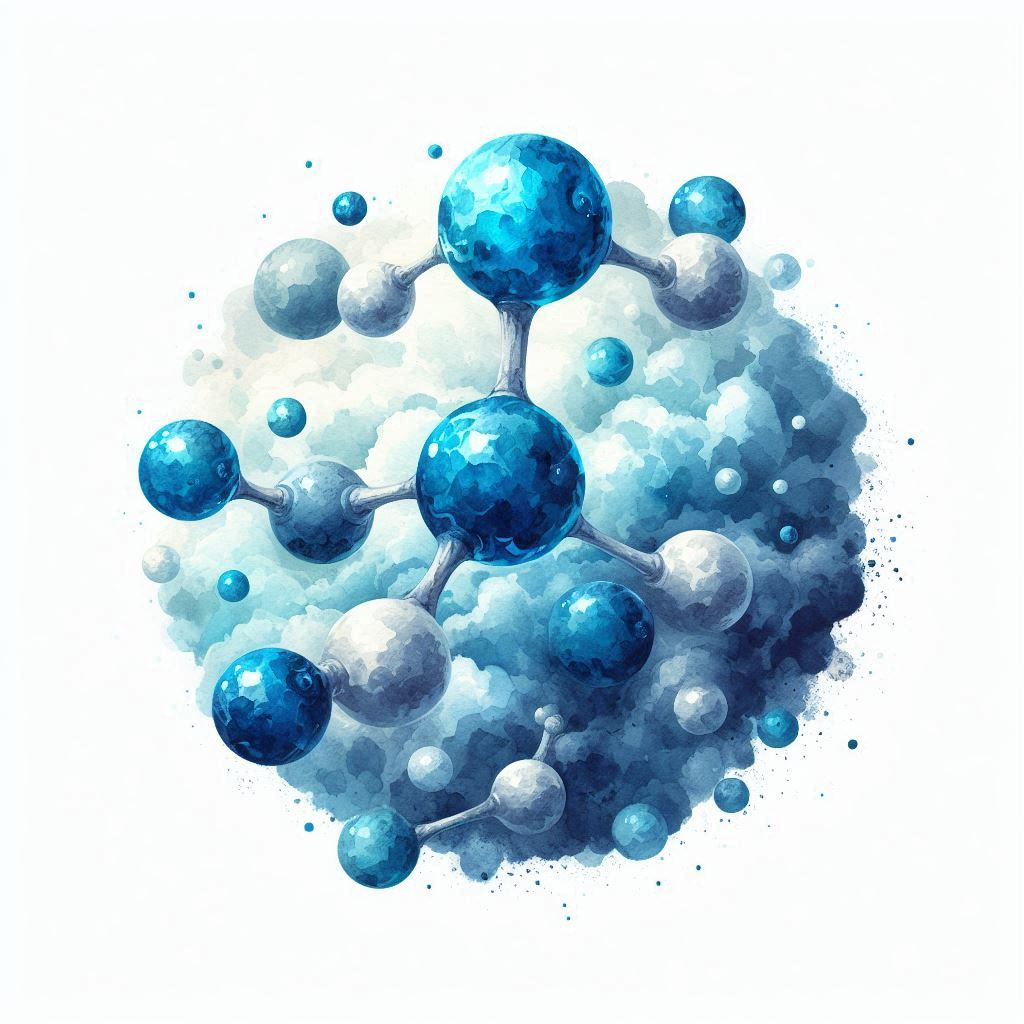
\includegraphics[width=0.7\textwidth]{cover2.jpg}
\end{figure}
\rule{0.8\textwidth}{0.02cm}\\

Jiří Janoš, Tomáš Jíra\\

\end{center}
\vfill
\begin{flushright}
\rule{3cm}{0.01cm} \\
Created in \LaTeX \\
\copyright \hspace{0.1cm} Prague 2024 \\
Version from \today
%\vspace{2cm}
\end{flushright}
\end{titlepage}
% Nasledující v tuto chvíli není potřeba, je uděláno automaticky pomocí \frontmatter
%\pagestyle{plain}
%\pagenumbering{roman}
%\setcounter{page}{3}

% OBSAH
{ \hypersetup{hidelinks} \tableofcontents }

\chapter{Introduction}
\label{kap:uvod}
Lets code everything!

\section{Brief introduction to Python}
\subsection{Importing packages}
\begin{lstlisting}[language=Python, style=mystyle2]
import numpy as np
\end{lstlisting}

\chapter{Brief introduction to Python}
\label{kap:python}
Students can learn the basics of Python in online courses like \href{https://www.learnpython.org/}{learnpython.org}.

Python is a modern, general-purpose programming language widely used for scientific computing and numerical simulations. Python's simplicity and readability make it an excellent choice for beginners.

One of the main advantages of Python is the availability of a wide range if libraries such as NumPy or SciPy for scientific purposes or MatPlotLib for plotting.

In this chapter, we will very briefly describe some basics of Python with emphasis on libraries we will need throughout the text. However, this introduction is not intended to explain Python from the beginning, as this is done in multitude of resources, such as \href{https://www.learnpython.org/}{\texttt{learnpython.org}}.

\textbf{We assume that the student is familiar with basic Python and understands loops. Thus we provide just a brief overview how to use python with the NumPy library.}

\begin{lstlisting}[language=Python, style=mystyle2]
import numpy as np
\end{lstlisting}


Calling functions from a Python library, e.g. number $\pi$, is done as follows:
\begin{lstlisting}[language=Python, style=mystyle2]
pi = np.pi
\end{lstlisting}
of if we want to take absolute value of a number
\begin{lstlisting}[language=Python, style=mystyle2]
number = np.abs(-1)
\end{lstlisting}



\section{Installing NumPy}
To use NumPy, you must first install it. You can do this by running the following command in your terminal or command prompt:
\begin{lstlisting}[language=Python, style=mystyle2]
pip install numpy
\end{lstlisting}

\section{Basic Python Concepts}
Before diving into NumPy, it is helpful to understand a few basic Python concepts:
\begin{itemize}
    \item \textbf{Variables:} Variables in Python are dynamically typed, meaning they do not need explicit declaration.
    \begin{lstlisting}[language=Python, style=mystyle2]
x = 5   # An integer
y = 2.5 # A floating point number
name = "Simulation" # A string
    \end{lstlisting}
    \item \textbf{Loops:} Python uses indentation to define blocks of code, making it simple to write loops.
    \begin{lstlisting}[language=Python, style=mystyle2]
for i in range(5):
    print(i)
    \end{lstlisting}
    \item \textbf{Functions:} Python functions are defined using the \texttt{def} keyword.
    \begin{lstlisting}[language=Python, style=mystyle2]
def add(a, b):
    return a + b
    \end{lstlisting}
\end{itemize}

\section{NumPy Basics}
NumPy is the core library for numerical computing in Python. It provides support for large, multi-dimensional arrays and matrices, along with a collection of mathematical functions to operate on these arrays efficiently.

\subsection{Creating Arrays}
The fundamental object in NumPy is the \texttt{array}. You can create an array using the \texttt{np.array()} function.
\begin{lstlisting}[language=Python, style=mystyle2]
import numpy as np

# Creating a 1D array
a = np.array([1, 2, 3, 4])

# Creating a 2D array (matrix)
b = np.array([[1, 2], [3, 4]])

print(a)
print(b)
\end{lstlisting}

\subsection{Array Operations}
NumPy allows you to perform element-wise operations on arrays, making it easy to work with large datasets.
\begin{lstlisting}[language=Python, style=mystyle2]
# Element-wise operations
c = a * 2    # Multiply each element of 'a' by 2
d = a + 10   # Add 10 to each element of 'a'

# Array addition
e = np.array([1, 2, 3, 4])
f = a + e    # Add corresponding elements of 'a' and 'e'
\end{lstlisting}

\subsection{Array Indexing and Slicing}
You can access elements of a NumPy array using indexing or slicing. This allows for efficient extraction of data from arrays.
\begin{lstlisting}[language=Python, style=mystyle2]
# Accessing an element
x = a[0]     # First element of 'a'

# Slicing an array
sub_array = a[1:3]  # Elements from index 1 to 2 (excluding 3)
\end{lstlisting}

\subsection{Useful Functions for Simulations}
NumPy provides several functions that are useful for numerical simulations, such as:
\begin{itemize}
    \item \texttt{np.linspace()}: Generates evenly spaced numbers over a specified range.
    \item \texttt{np.random.random()}: Generates random numbers.
    \item \texttt{np.dot()}: Performs matrix multiplication.
\end{itemize}

\begin{lstlisting}[language=Python, style=mystyle2]
# Generating an array of 5 numbers between 0 and 10
x = np.linspace(0, 10, 5)

# Creating a 2x2 matrix of random numbers
random_matrix = np.random.random((2, 2))

# Matrix multiplication
result = np.dot(b, random_matrix)
\end{lstlisting}



\mainmatter

\part{Electronic structure theory}
\label{part:elstruc}
This part provides an educational exploration into the computational techniques fundamental to understanding molecular electronic structure in quantum chemistry. Beginning with the \acrfull{hf} method, the text introduces this foundational approach for determining molecular orbitals and electronic energies by approximating the interactions of electrons through a mean-field approximation. The HF method forms the basis for subsequent methods and is presented with a practical coding exercise that guides readers in implementing and calculating \acrshort{hf} energies in Python.

Moving beyond HF, the text delves into \acrfull{mppt}, which improves \acrshort{hf} predictions by introducing corrections for electron correlation through a perturbative approach. This section includes exercises on calculating second- and third-order corrections, allowing readers to enhance their understanding of how electron interactions can be more accurately incorporated. \acrfull{ci} theory is then presented as an approach for representing the molecular wavefunction as a combination of electron configurations. Here, readers learn the theoretical basis of \acrshort{ci} and engage with practical examples focused on constructing the \acrshort{ci} Hamiltonian matrix and solving for molecular energies, particularly emphasizing \acrfull{fci} for high accuracy in small systems.

The part culminates with a discussion on the \acrfull{cc} theory, a highly accurate and computationally efficient method for capturing electron correlation effects, often used for small to medium-sized systems. By introducing truncations such as \acrfull{ccd} and \acrfull{ccsd}, the text demonstrates how electron correlation can be systematically included while balancing computational cost. The \acrshort{cc} section provides iterative coding exercises for calculating correlation energies, rounding out the document's comprehensive approach to electronic structure methods in computational quantum chemistry. Through this blend of theory, mathematical formulations, and hands-on coding exercises, the document serves as an invaluable resource for building a strong foundational understanding of electronic structure methods.


\chapter{Hückel theory}
\label{kap:huckel}
\acrfull{ht} is one of the first and probably also the simplest methods to solve the electronic structure of molecules. It ranks among semiempirical quantum chemical methods as it contains empirical parameters parametrized to experiments or high-level calculations. The strength of \acrshort{ht} lies in its simplicity because it allows to solve the secular equations using a pen-and-paper approach, which makes it excellent for education purposes. The downside of \acrshort{ht} is, on the contrary, its applicability to only frontier molecular orbitals. The most famous applications of \acrshort{ht} are unsaturated polyens such as buta-1,3-diene or benzene. Although these small molecules can be solved with only a pen and paper, \acrshort{ht} is applicable also to larger systems such as molecular rotors or porphyrins. In this Chapter, we will use \acrshort{ht} as a warm-up for the next more advanced electronic structure chapters and show how to calculate \acrshort{ht} for an arbitrary conjugated planar system.

\section{Theoretical background}

The \acrshort{ht} is a one-particle theory (mean-field such as \acrlong{hf}) and considers the electronic Hamiltonian to be approximated as a sum of effective one-particle hamiltonians $\hat{h}_{i, \mathrm{eff}}$:
\begin{equation}
\hat{H}_{\mathrm{HT}}= \sum \hat{h}_{i, \mathrm{eff}} \, .
\label{eq:huckel1}
\end{equation}
The one-particle Hamiltonian is defined with an effective potential as
\begin{equation}
\hat{h}_{i, \mathrm{eff}}  = -\frac{1}{2}\nabla_i^2  - \sum_j \frac{Z_j}{|\Vec{r}_i - \Vec{R}_j|} + V(\Vec{r}_{i, \mathrm{eff}})  \, ,
\label{eq:huckel2}
\end{equation}
where $j$ is the index of the nuclei, $Z_j$ is the charge of a nucleus and $\Vec{r}_i$ and $\Vec{R}_j$ are the positions of the electrons and nuclei respectively.

The electronic wave function in \acrshort{ht} is expressed as a linear combination of atomic orbitals $\phi_\nu$,
\begin{equation}
\psi= \sum_\nu c_\nu \phi_\nu \, ,
\label{eq:huckel3}
\end{equation}
where the index $\nu$ runs over all the basis functions. The spirit of the \acrshort{ht} lies in the selection of the basis, which comprises only a selected set of the frontier atomic orbitals. For describing conjugated systems, only the $p$ orbitals perpendicular to the conjugation plane are taken. This truncation is the core limitation of the theory as it cannot go beyond the selected set of frontier orbitals but it is also what greatly simplifies the working equations. Applying the variational principle to the wave function leads to secular equations, written in a matrix as
\begin{equation}
\mathbf{H}\Vec{c}=\varepsilon \mathbf{S}\Vec{c} \, ,
\label{eq:huckel4}
\end{equation}
where $\varepsilon$ is the energy corresponding to the molecular orbital, $\mathbf{H}$ is the Hamiltoninan matrix with elements defined as expectation vlues of the one-electron Hamiltonian and the basis functions
\begin{equation}
H_{\nu\mu} = \langle \phi_\nu | \hat{h}_{i, \mathrm{eff}} | \phi_\mu \rangle \, ,
\label{eq:huckel5}
\end{equation}
$\mathbf{S}$ is the overlap matrix,
\begin{equation}
S_{\nu\mu} = \langle \phi_\nu | \phi_\mu \rangle \, ,
\label{eq:huckel6}
\end{equation}
and $\Vec{c}$ is the vector of the expansion coefficients.

The second series of approximations in \acrshort{ht} (the first is the truncation of the basis set) is on the elements of the Hamiltonian and overlap matrices:
\begin{itemize}
    \item The basis set is considered orthonormal. Thus, the overlap matrix is unitary, that is, $S_{\nu\mu} = \delta_{\nu\mu}$.
    \item The diagonal terms of the Hamiltonian matrix are equal to a predefined parameter,  $H_{\nu\nu} = \alpha$.
    \item If the basis functions $\phi_\nu$ and $\phi_\mu$ reside in neighboring atoms, that is, atoms linked by a chemical bond, the Hamiltonian matrix element is set to another predefined parameter, $H_{\nu\mu} = \beta$.
    \item If the basis functions $\phi_\nu$ and $\phi_\mu$ reside in atoms that are not linked by a chemical bond, the Hamiltonian matrix element is zero, $H_{\nu\mu} = 0$.
\end{itemize}
The parameters $\alpha$ and $\beta$ are usually parameterized from experiments. The value of $\alpha$ is $\SI{-11.4}{\ev}$ which is the carbon ionization energy. The parameter $\beta$ can acquire quite different values based on the parametrization. Using spectroscopic data gives $\beta = \SI{-3.48}{\eV}$, while thermochemistry yields $\beta = \SI{-0.78}{\ev}$. The parameterization depends on the purpose of our calculations. If we intend to calculate energy gaps between HOMO and LUMO orbitals, we will rather take the value obtained from spectroscopy and vice versa.

Taking all the approximations on the matrix elements together, the final working equations of the \acrlong{ht} are 
\begin{equation}
\mathbf{H}\Vec{c}=\varepsilon\Vec{c}\, ,
\label{eq:huckel7}
\end{equation}
We can recognize this as an eigenvalue equation which is solve by diagonalization of the Hamiltonian matrix. The energies $\varepsilon$ are the eigenvalues and the expansion coefficients $\Vec{c}$ are their corresponding eigenvectors. The Hamiltonian matrix has the parameter $\alpha$ on the diagonal and the parameter $\beta$ at the place corresponding to the neighboring atoms. 

To illustrate the form of $\mathbf{H}$ on a simple example, we will use the famous textbook case: buta-1,3-diene. If we label the atoms as \ce{C_1=C_2-C_3=C_4}, the Hamiltonian matrix reads
\begin{equation}
\mathbf{H} = 
\begin{pmatrix}
\alpha & \beta & 0 & 0  \\
\beta &\alpha & \beta & 0  \\
0 &\beta &\alpha & \beta  \\
0 & 0 & \beta &\alpha  
\end{pmatrix}
\label{eq:huckel8}
\end{equation}
It is a common trick to make a substitution $\varepsilon = \alpha - \beta x$ and divide the both sides of the equation by $\beta$ which leads to
\begin{equation}
\begin{pmatrix}
0 & 1 & 0 & 0  \\
1 & 0 & 1 & 0  \\
0 & 1 & 0 & 1  \\
0 & 0 & 1 & 0  
\end{pmatrix}\Vec{c}=x\Vec{c}\, .
\label{eq:huckel9}
\end{equation}
The new matrix is then diagonalized with the eigenvalues corresponding to $x$ and the eigenvectors still being the same expansion coefficients. The energies are recovered from $\varepsilon = \alpha - \beta x$. The main advantage is that this procedure does not require specifying $\alpha$ and $\beta$ a priori. We calculate the energy levels in terms of parameters $\alpha$ and $\beta$ for any system, and then we can try to parameterize them. 
Construction of the new matrix is even simpler than constructing the Hamiltonian matrix. The diagonal contains all zeros and all the elements corresponding to the neighbouring atoms are 1 instead of $\beta$.

\section{Numerical implementation}

The numerical implementation of \acrlong{ht} is very simple and requires only diagonalization of either the Hamiltonian matrix or the matrix using 1 instead of $\beta$ and 0 instead of $\alpha$. The diagonalization can be performed with NumPy's routines such as \python{np.linalg.eig(H)} which provides both the eigenvalues and eigenvectors:
\begin{lstlisting}[language=Python, style=mystyle2]
eigenvalues, eigenvectors = np.linalg.eigh(H)
\end{lstlisting}
where the eigenvectors are the columns of the eigenvector matrix, see the \href{https://numpy.org/doc/2.1/reference/generated/numpy.linalg.eig.html}{NumPy manual}. Since the matrix is Hermitian, algorithms tailored for such matrices like \python{np.linalg.eigh(H)} can be used.

The implementation of \acrshort{ht} is simple and we leave the coding fully to the student and provide only one possible author solution at the end of the book.

\section{Applications}

\subsection*{Exercise: Benchmarking the code on buta-1,3-diene}

The \acrlong{ht} for buta-1,3-diene yields the following orbital energies 
\begin{equation*}
\begin{split}
\varepsilon_1 &= \alpha+1.62\beta \, ,\\
\varepsilon_2 &= \alpha+0.62\beta \, ,\\
\varepsilon_3 &= \alpha-0.62\beta \, ,\\
\varepsilon_4 &= \alpha-1.62\beta \, ,
\end{split}
\end{equation*}
and wave functions
\begin{equation*}
\begin{split}
\psi_1 &= 0.37\phi_1+0.60\phi_2+0.60\phi_3+0.37\phi_4 \, ,\\
\psi_2 &= 0.60\phi_1+0.37\phi_2-0.37\phi_3-0.60\phi_4 \, ,\\
\psi_3 &= 0.60\phi_1-0.37\phi_2-0.37\phi_3+0.60\phi_4 \, ,\\
\psi_4 &= 0.37\phi_1-0.60\phi_2+0.60\phi_3-0.37\phi_4 \, .
\end{split}
\end{equation*}
In this Exercise, we will use this analytic result to benchmark the implemented code for \acrshort{ht}.

\paragraph{Assignment:} Calculate the orbital energies $\varepsilon$ and expansion coefficients $\Vec{c}$, and compare them with the analytic solution to confirm a correct implementation of the \acrlong{ht}. Additionaly, use the parameters $\alpha = \SI{-11.4}{\ev}$ and $\beta = \SI{-3.48}{\eV}$ to predict the excitation energy of buta-1,3-diene.

\subsection*{Exercise: Excitation energies of benzene, naphthalene and phenanthrene}

The \acrlong{ht} can be applied effectively to conjugated systems of aromatic rings such as benzene, naphthalene or phenanthrene. Frontier molecular orbitals in these systems are composed of the $\pi$ bonding and antibonding orbitals which can be well captured by \acrshort{ht}. In this Exercise, we will try to predict the structure of the conjugated system of aromatic compounds and their excitation energies. 

\begin{figure}[ht!]
    \centering
    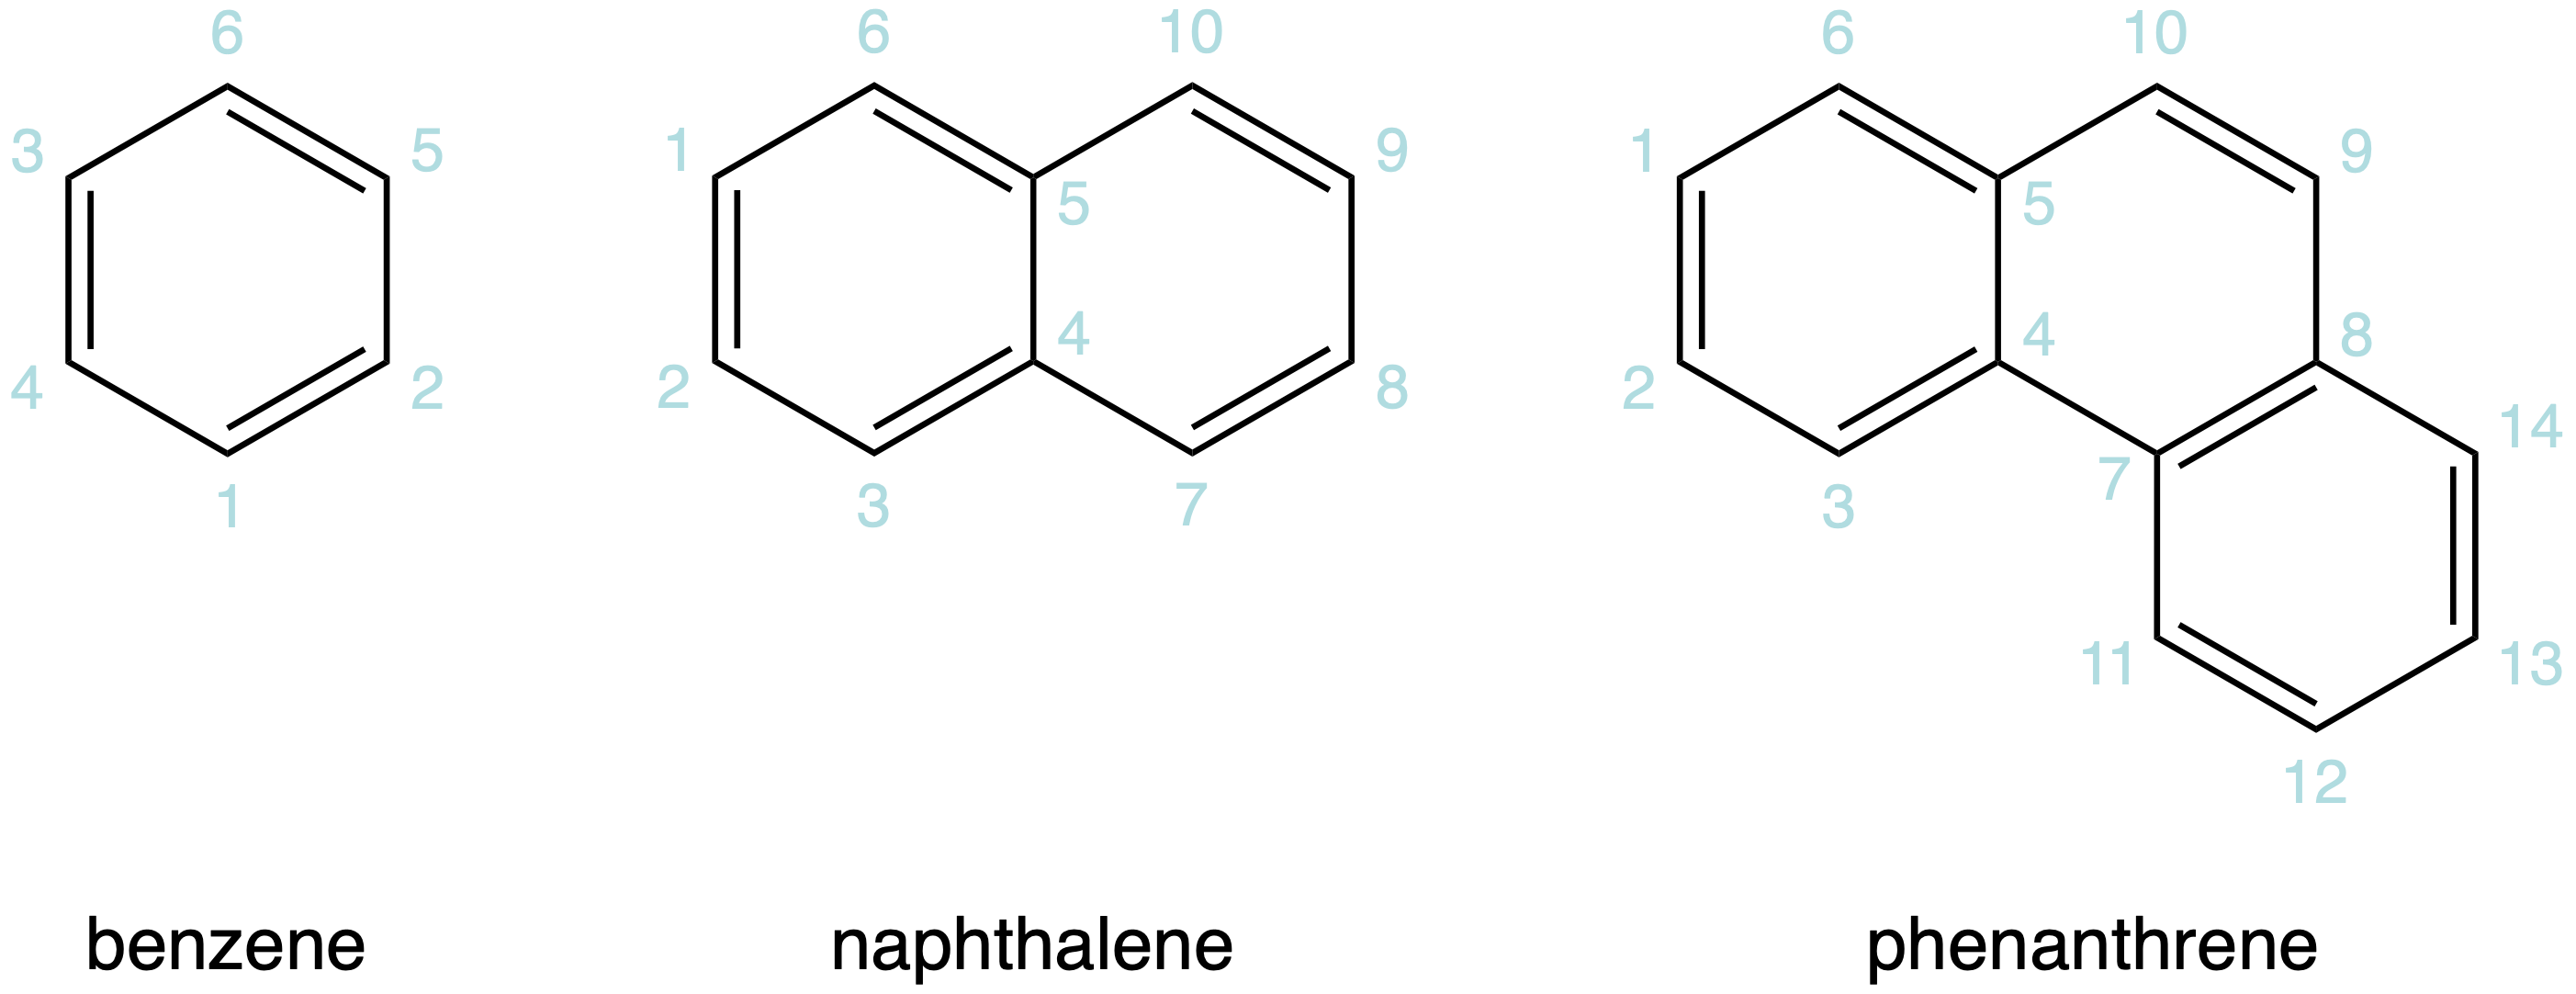
\includegraphics[width=0.6\linewidth]{scriptum/obrazky/huckel/ex2.png}
    % \caption{Str}
    \label{fig:huckel1}
\end{figure}

\paragraph{Assignment:} Calculate the orbital energies $\varepsilon$ and expansion coefficients $\Vec{c}$ for benzene, naphthalene and phenanthrene. Try to plot the orbitals and compare them with literature or \acrlong{hf} calculations. Then, calculate the energy gap between the HOMO and LUMO orbitals using $\alpha = \SI{-11.4}{\ev}$ and $\beta = \SI{-3.48}{\eV}$ and predict excitation energies. Do they compare to experimental values? Do you see the same trends? 

\subsection*{Exercise: Excitation energy of porphyrin and its HOMO and LUMO}

Porphyrin is one of the building blocks of life and is often used in nature to capture photons. Its conjugated system of double bonds is responsible for a shift of the absorption spectrum to the visible region. Both HOMO and LUMO are mainly composed of $p$ orbitals on carbons and nitrogen. In this Exercise, we will test the predictability of \acrshort{ht} on bare porphyrin. 

\begin{figure}[ht!]
    \centering
    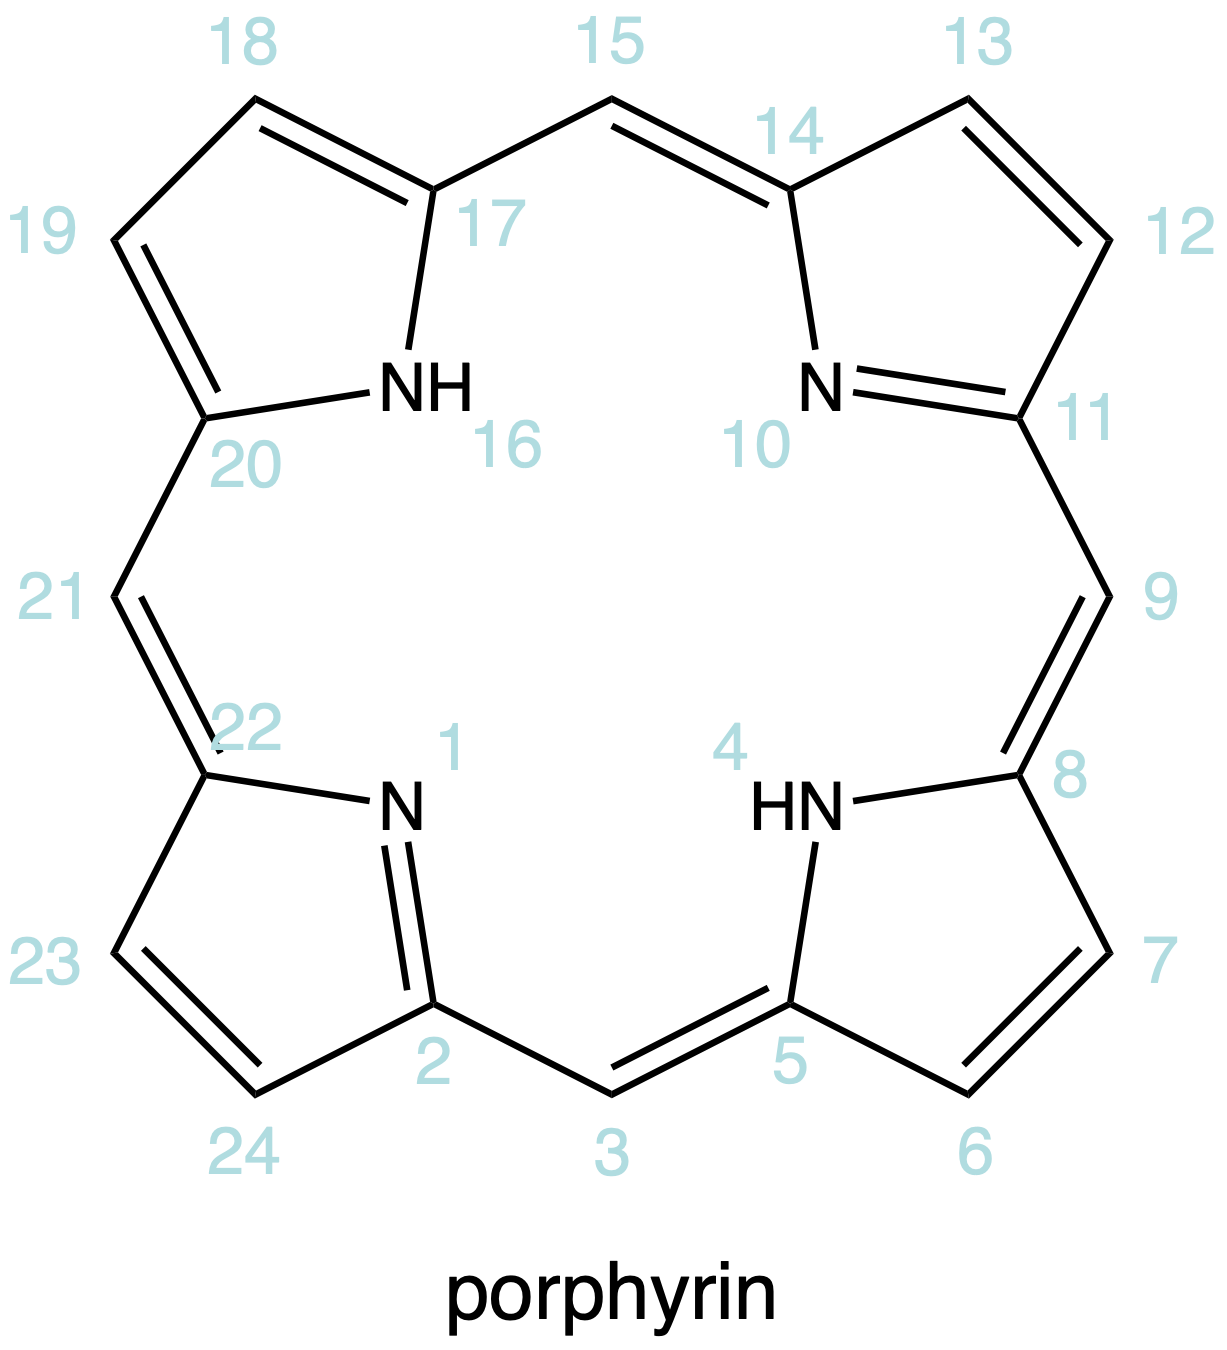
\includegraphics[width=0.3\linewidth]{scriptum/obrazky/huckel/ex3.png}
    % \caption{Str}
    \label{fig:huckel1}
\end{figure}

\paragraph{Assignment:} Calculate the orbital energies $\varepsilon$ and expansion coefficients $\Vec{c}$ for porphyrin. Plot the orbitals and compare them with literature or \acrlong{hf} calculations. Then, calculate the energy gap between HOMO and LUMO orbitals using $\alpha = \SI{-11.4}{\ev}$ and $\beta = \SI{-3.48}{\eV}$ and predict excitation energies. Do they compare to experimental values?

\chapter{Hartree--Fock Method}

The \acrfull{hf} method stands as a cornerstone in quantum chemistry, offering a systematic approach to solve the electronic structure problem in molecules. This computational technique strives to determine the optimal wave function for a given molecular system, providing insights into the distribution of electrons and their energies.

\section{Theoretical Background}

Our primary focus is on solving the Schrödinger equation in the following form:

\begin{equation}
\hat{\mathbf{H}}\ket{\Psi}=E\ket{\Psi},
\end{equation}

where \(\hat{\mathbf{H}}\) denotes the molecular Hamiltonian operator, \(\ket{\Psi}\) represents the molecular wave function, and \(E\) is the total energy of the system. The \acrshort{hf} method aims to approximate the wave function \(\ket{\Psi}\) using a single Slater determinant, which can be expressed as:

\begin{equation}
\ket{\Psi}=\ket{\chi_1\chi_2\cdots\chi_N},
\end{equation}

where \(\chi_i\) indicates a molecular spin orbital and \(N\) is the total number of electrons. The goal of the \acrshort{hf} method is to optimize these molecular orbitals in order to minimize the system's total energy, thereby providing a reliable estimate of the electronic structure.

In the \acrfull{rhf} method, a constraint is placed on the electron spin, allowing us to work with spatial orbitals instead of spin orbitals. This enables us to express the Slater determinant in terms of spatial orbitals as follows:

\begin{equation}
\ket{\Psi}=\ket{\Phi_1\Phi_2\cdots\Phi_{N/2}},
\end{equation}

where \(\Phi_i\) represents a molecular spatial orbital. It is evident that, for the \acrshort{rhf} method, the system must contain an even number of electrons. In practical calculations, it is often convenient to expand the molecular orbitals (whether spin or spatial) in terms of basis functions \(\phi\), typically represented as sums of Gaussian functions, and to work with the corresponding expansion coefficients. Assuming that the wave function can be expressed as a single Slater determinant, we expand our molecular orbitals in terms of these basis functions and optimize the energy of the determinant, leading us to the Roothaan equations given by:

\begin{equation}\label{eq:roothaan}
\mathbf{FC}=\mathbf{SC}\bm{\varepsilon},
\end{equation}

where \(\mathbf{F}\) is the Fock matrix (to be defined later), \(\mathbf{C}\) is a matrix of orbital coefficients, \(\mathbf{S}\) is the overlap matrix (also to be defined later), and \(\bm{\varepsilon}\) represents the orbital energies.

\section{Implementation of the Restricted Hartree--Fock Method}

Let us begin by defining the core Hamiltonian, also referred to as the one-electron Hamiltonian. The core Hamiltonian constitutes a portion of the full Hamiltonian that omits electron-electron repulsion. In index notation, it is expressed as

\begin{equation}\label{eq:hamiltonian}
H_{\mu\nu}^{core}=T_{\mu\nu}+V_{\mu\nu}
\end{equation}

where \(\mu\) and \(\nu\) are indices of basis functions, \(T_{\mu\nu}\) denotes a kinetic energy matrix element and \(V_{\mu\nu}\) denotes a potential energy matrix element. These matrix elements given as

\begin{align}
T_{\mu\nu}&=\braket{\phi_{\mu}|\hat{T}|\phi_{\nu}} \\
V_{\mu\nu}&=\braket{\phi_{\mu}|\hat{V}|\phi_{\nu}}
\end{align}

are usually calculated using analytical expressions. Additionally, using analytical expressions, we can calculate the overlap integrals

\begin{equation}\label{eq:overlap}
S_{\mu\nu}=\braket{\phi_{\mu}|\phi_{\nu}}
\end{equation}

and the two-electron Coulomb repulsion integrals

\begin{equation}\label{eq:coulomb}
J_{\mu\nu\kappa\lambda}=\braket{\phi_{\mu}\phi_{\mu}|\hat{J}|\phi_{\kappa}\phi_{\lambda}},
\end{equation}

which play crucial roles in the \acrshort{hf} calculation.\cite{10.1016/S0065-3276!08!60019-2} The \acrshort{hf} method revolves around solving the Roothaan equations \eqref{eq:roothaan} iteratively. The Fock matrix is defined as

\begin{equation}\label{eq:fock}
F_{\mu\nu}=H_{\mu\nu}^{core}+D_{\kappa\lambda}(J_{\mu\nu\kappa\lambda}-\frac{1}{2}J_{\mu\lambda\kappa\nu})
\end{equation}

depends on the unknown density matrix \(\mathbf{D}\). This iterative process is carried out through a \acrfull{scf} method. In each iteration, a guess for the density matrix is made, and the Roothaan equations are solved. The density matrix is then updated as

\begin{equation}
D_{\mu\nu}=2C_{\mu i}C_{\nu i}
\end{equation}

and the total energy of the system

\begin{equation}
E=\frac{1}{2}D_{\mu\nu}(H_{\mu\nu}^{core}+F_{\mu\nu})+E_{nuc}
\end{equation}

is then calculated using the core Hamiltonian and the Fock matrix. The important thing to note is that the Fock matrix depends on the density matrix, which is updated in each iteration. The initial guess for the density matrix is often set to zero. After the density matrix and the total energy are converged, the \acrshort{scf} procedure is terminated, and the optimized molecular orbitals are obtained. To get the final energy of the system, we need to add the nuclear repulsion energy of the form

\begin{equation}
E_{nuc}=\sum_{A}\sum_{B<A}\frac{Z_{A}Z_{B}}{R_{AB}},
\end{equation}

where \(Z_A\) is the nuclear charge of atom A, and \(R_{AB}\) is the distance between atoms A and B.

\subsection{Gradient of the Restricted Hartree--Fock Method}

If we perform the calculation as described above and get the density matrix \(\mathbf{D}\) we can evaluate the nuclear energy gradient as\cite{10.1002/9780470749593.hrs006}

\begin{equation}
\frac{\partial E}{\partial X_{A,i}}=D_{\mu\nu}\frac{\partial H_{\mu\nu}^{core}}{\partial X_{A,i}}+2D_{\mu\nu}D_{\kappa\lambda}\frac{\partial J_{\mu\nu\kappa\lambda}}{\partial X_{A,i}}-2W_{\mu\nu}\frac{\partial S_{\mu\nu}}{\partial X_{A,i}}
\end{equation}

where \(i\) is the index of the coordinate and where \(\mathbf{W}\) is energy weighed density matrix defined as

\begin{equation}
W_{\mu\nu}=2C_{\mu i}C_{\nu i}\varepsilon_i
\end{equation}

\section{\texorpdfstring{Integral Transforms to the Basis of Molecular Spinorbitals\label{sec:integral_transform}}{Integral Transforms to the Basis of Molecular Spinorbitals}}

To perform most of the \acrfull{post-hf} calculations, we usually need to transform the integrals to the \acrfull{ms} basis. We will describe it here and refer to it in the \acrshort{post-hf} methods sections. We will also present the \acrshort{post-hf} methods using the integrals in the \acrshort{ms} basis (and its antisymmetrized form in case of the Coulomb integrals), since it is more general.

All the integrals defined in the equations \eqref{eq:hamiltonian}, \eqref{eq:overlap}, and \eqref{eq:coulomb} and even the Fock matrix in the equation \eqref{eq:fock} are defined in the basis of atomic orbitals. To transform these integrals to the \acrshort{ms} basis, we need to use the coefficient matrix \(\mathbf{C}\) obtained from the solution of the Roothaan equations \eqref{eq:roothaan}. The coefficient matrix \(\mathbf{C}\), which is obtained from the \acrshort{rhf} calculation, is calculated in the spatial molecular orbital basis. The first step is to expand the coefficient matrix \(\mathbf{C}\) to the \acrshort{ms} basis. This can be done mathematically using the tiling matrix \(\mathbf{P}_{n\times 2n}\), defined as

\begin{equation}
\mathbf{P}=
\begin{pmatrix}
e_1&e_1&e_2&e_2&\dots&e_n&e_n
\end{pmatrix}
,
\end{equation}

where \(e_i\) represents the \(i\)-th column of the identity matrix \(\mathbf{I}_n\) and the matrices \(\mathbf{M}_{n\times 2n}\) and \(\mathbf{N}_{n\times 2n}\) with elements given by

\begin{equation}
M_{ij}=1-j\bmod 2,N_{ij}=j \bmod 2.
\end{equation}

The coefficient matrix \(\mathbf{C}\) in the MS basis can be then expressed as

\begin{equation}
\mathbf{C}^{MS}=
\begin{pmatrix}
\mathbf{CP} \\
\mathbf{CP}
\end{pmatrix}
\odot
\begin{pmatrix}
\mathbf{M} \\
\mathbf{N}
\end{pmatrix}
,
\end{equation}

where \(\odot\) denotes the Hadamard product. This transformed matrix \(\mathbf{C}^{MS}\) is then used to transform the Coulomb integrals \(\mathbf{J}\) to the MS basis as

\begin{equation}
J_{pqrs}^{MS}=C_{\mu p}^{MS}C_{\nu q}^{MS}(\mathbf{I}_{2}\otimes_K(\mathbf{I}_{2}\otimes_K\mathbf{J})^{(4,3,2,1)})_{\mu\nu\kappa\lambda}C_{\kappa r}^{MS}C_{\lambda s}^{MS},
\end{equation}

where the superscript \((4,3,2,1)\) denotes the axes transposition and \(\otimes_K\) is the Kronecker product. This notation accounts for the spin modifications and ensures that the transformations adhere to quantum mechanical principles. We also define the antisymmetrized Coulomb integrals in physicists' notation as

\begin{equation}
\braket{pq||rs}=(J_{pqrs}^{MS}-J_{psrq}^{MS})^{(1,3,2,4)}.
\end{equation}

For the transformation of the one-electron integrals such as the core Hamiltonian, the overlap matrix and also the Fock matrix, we use the formula

\begin{equation}
A_{pq}^{MS}=C_{\mu p}^{MS}(\mathbf{I}_{2}\otimes_K\mathbf{A})_{\mu\nu}C_{\nu q}^{MS},
\end{equation}

where \(\mathbf{A}\) is an arbitrary one-electron integral. Since a lot of the \acrshort{post-hf} methods also use differences of orbital energies in the denominator, it is practical to define the tensors

\begin{align}
\varepsilon^{a}_{i}&=\varepsilon_i-\varepsilon_a \\
\varepsilon^{ab}_{ij}&=\varepsilon_i+\varepsilon_j-\varepsilon_a-\varepsilon_b \\
\varepsilon^{abc}_{ijk}&=\varepsilon_i+\varepsilon_j+\varepsilon_k-\varepsilon_a-\varepsilon_b-\varepsilon_c,
\end{align}

where \(a\), \(b\), \(c\) are virtual orbitals and \(i\), \(j\), \(k\) are occupied orbitals. These tensors make the code more readable, easier to understand and also more efficient.

\section{\texorpdfstring{Hartree--Fock Method and Integral Transform Coding Exercise\label{sec:hf_int_code_exercise}}{Hartree--Fock Method and Integral Transform Coding Exercise}}

This section provides code snippets for the \acrshort{hf} method and the integral transforms to the \acrshort{ms} basis. The code snippets are written in Python and use the NumPy package for numerical calculations. The exercises are designed to help you understand the implementation of the \acrshort{hf} method and the transformation of integrals to the \acrshort{ms} basis. The solutions are provided in Section \ref{sec:code_solutions} to guide you through the implementation process and ensure that you can verify your results.

The exercise codes are designed to be self-contained and can be run in any Python environment. They contain placeholders that you need to fill in to complete the implementation. The exercises assume that you have defined the \texttt{\lstinline!atoms!}, \texttt{\lstinline!coords!}, \texttt{\lstinline!S!}, \texttt{\lstinline!H!}, and \texttt{\lstinline!J!} variables, which represent the list of atomic numbers, atomic coordinates, overlap matrix, core Hamiltonian, and Coulomb integral tensor, respectively. These variables can be generaly obtained from a .xyz molecule file and the output of a quantum chemistry software. If you want to just get to the coding part, you can save the \textattachfile[color=0 0 1]{molecule.xyz}{molecule.xyz}, \textattachfile[color=0 0 1]{S_AO.mat}{S\_AO.mat}, \textattachfile[color=0 0 1]{H_AO.mat}{H\_AO.mat}, and \textattachfile[color=0 0 1]{J_AO.mat}{J\_AO.mat} files to the same directory as the exercise codes and load the variables using the Listing \ref{code:load_exercise} below. The \texttt{\lstinline!ATOM!} variable is a dictionary that maps the atomic symbols to atomic numbers.

\raggedbottom\begin{lstlisting}[language=Python, caption={Example loading of molecule and integrals over atomic basis functions into variables used throughout exercises.}, label=code:load_exercise]
# get the atomic numbers and coordinates of all atoms
atoms = np.array([ATOM[line.split()[0]] for line in open("molecule.xyz").readlines()[2:]], dtype=int)
coords = np.array([line.split()[1:] for line in open("molecule.xyz").readlines()[2:]], dtype=float)

# convert to bohrs
coords *= 1.8897261254578281

# load the integrals from the files
H, S = np.loadtxt("H_AO.mat", skiprows=1), np.loadtxt("S_AO.mat", skiprows=1); J = np.loadtxt("J_AO.mat", skiprows=1).reshape(4 * [S.shape[1]])
\end{lstlisting}

With all the variables defined, you can proceed to the \acrshort{hf} exercise in the Listing \ref{code:hf_exercise} below.

\raggedbottom\begin{lstlisting}[language=Python, caption={\acrshort{hf} method exercise code.}, label=code:hf_exercise]
"""
Here are defined some of the necessary variables. The variable "E_HF" stores the Hartree-Fock energy, while "E_HF_P" keeps track of the previous iteration's energy to monitor convergence. The "thresh" defines the convergence criteria for the calculation. The variables "nocc" and "nbf" represent the number of occupied orbitals and the number of basis functions, respectively. Initially, "E_HF" is set to zero and "E_HF_P" to one to trigger the start of the Self-Consistent Field (SCF) loop. Although you can rename these variables, it is important to note that certain sections of the code are tailored to these specific names.
"""
E_HF, E_HF_P, nocc, nbf, thresh = 0, 1, sum(atoms) // 2, S.shape[0], 1e-8

"""
These lines set up key components for our HF calculations. We initialize the density matrix as a zero matrix, and the coefficients start as an empty array. Although the coefficient matrix is computed within the while loop, it's defined outside to allow for its use in subsequent calculations, such as the MP energy computation. Similarly, the exchange tensor is accurately calculated here by transposing the Coulomb tensor. The "eps" vector, which contains the orbital energies, is also defined at this stage to facilitate access throughout the script. This setup ensures that all necessary variables are ready for iterative processing and further calculations beyond the SCF loop.
"""
K, F, D, C, eps = J.transpose(0, 3, 2, 1), np.zeros_like(S), np.zeros_like(S), np.zeros_like(S), np.array(nbf * [0])

"""
This while loop is the SCF loop. Please fill it so it calculates the Fock matrix, solves the Fock equations, builds the density matrix from the coefficients and calculates the energy. You can use all the variables defined above and all the functions in numpy package. The recommended functions are np.einsum and np.linalg.eigh. Part of the calculation will probably be calculation of the inverse square root of a matrix. The numpy package does not conatin a function for this. You can find a library that can do that or you can do it manually. The manual calculation is, of course, preferred.
"""
while abs(E_HF - E_HF_P) > thresh:
    break

"""
In the followng block of code, please calculate the nuclear-nuclear repulsion energy. You should use only the atoms and coords variables. The code can be as short as two lines. The result should be stored in the "VNN" variable.
"""
VNN = 0

# print the results
print("RHF ENERGY: {:.8f}".format(E_HF + VNN))
\end{lstlisting}

If you are satisfied with the results, you can proceed to the next exercise in the Listing \ref{code:int_exercise} below, which involves transforming the integrals to the molecular spinorbital basis.

\raggedbottom\begin{lstlisting}[language=Python, caption={Integral transform exercise code.}, label=code:int_exercise]
"""
To perform most of the post-HF calculations, we need to transform the Coulomb integrals to the molecular spinorbital basis, so if you don't plan to calculate any post-HF methods, you can end the eercise here. The restricted MP2 calculation could be done using the Coulomb integral in MO basis, but for the sake of subsequent calculations, we enforce here the integrals in the MS basis. The first thing you will need for the transform is the coefficient matrix in the molecular spinorbital basis. To perform this transform using the mathematical formulation presented in the materials, the first step is to form the tiling matrix "P" which will be used to duplicate columns of a general matrix. Please define it here.
"""
P = np.zeros((nbf, 2 * nbf))

"""
Now, please define the spin masks "M" and "N". These masks will be used to zero out spinorbitals, that should be empty.
"""
M, N = np.zeros((nbf, 2 * nbf)), np.zeros((nbf, 2 * nbf))

"""
With the tiling matrix and spin masks defined, please transform the coefficient matrix into the molecular spinorbital basis. The resulting matrix should be stored in the "Cms" variable.
"""
Cms = np.zeros(2 * np.array(C.shape))

"""
For some of the post-HF calculations, we will also need the Hamiltonian and Fock matrix in the molecular spinorbital basis. Please transform it and store it in the "Hms" and "Fms" variable. If you don't plan to calculate the CCSD method, you can skip the transformation of the Fock matrix, as it is not needed for the MP2 and CI calculations.
"""
Hms, Fms = np.zeros(2 * np.array(H.shape)), np.zeros(2 * np.array(H.shape))

"""
With the coefficient matrix in the molecular spinorbital basis available, we can proceed to transform the Coulomb integrals. It is important to note that the transformed integrals will contain twice as many elements along each axis compared to their counterparts in the atomic orbital (AO) basis. This increase is due to the representation of both spin states in the molecular spinorbital basis.
"""
Jms = np.zeros(2 * np.array(J.shape))

"""
The post-HF calculations also require the antisymmetrized two-electron integrals in the molecular spinorbital basis. These integrals are essential for the MP2 and CC calculations. Please define the "Jmsa" tensor as the antisymmetrized two-electron integrals in the molecular spinorbital basis.
"""
Jmsa = np.zeros(2 * np.array(J.shape))

"""
As mentioned in the materials, it is also practical to define the tensors of reciprocal orbital energy differences in the molecular spinorbital basis. These tensors are essential for the MP2 and CC calculations. Please define the "Emss", "Emsd" and "Emst" tensors as tensors of single, double and triple excitation energies, respectively. The configuration interaction will not need these tensors, so you can skip this step if you don't plan to program the CI method. The MP methods will require only the "Emsd" tensor, while the CC method will need both tensors.
"""
Emss, Emsd = np.array([]), np.array([])
\end{lstlisting}

If you successfully completed the exercise, you can compare your results with the provided solutions. Solution to the \acrshort{rhf} method can be found in Section \ref{sec:hf_code_solution} and the solution to integral transform in Section \ref{sec:int_code_solution}. If you are satisfied with the results, you are now set for the post-HF methods exercises.
\chapter{Møller--Plesset Perturbation Theory}

\acrfull{mppt} is a quantum mechanical method used to improve the accuracy of electronic structure calculations within the framework of \acrshort{hf} theory. It involves treating electron-electron correlation effects as a perturbation to the reference \acrshort{hf} wave function. The method is named after its developers, physicists C. Møller and M. S. Plesset. By systematically including higher-order corrections, \acrshort{mppt} provides more accurate predictions of molecular properties compared to the initial \acrshort{hf} approximation.

\section{Theory of the Perturbative Approach}

As for the \acrshort{hf} method, we start with the Schrödinger equation in the form

\begin{equation}
\hat{\mathbf{H}}\ket{\Psi}=E\ket{\Psi},
\end{equation}

where \(\hat{\mathbf{H}}\) is the molecular Hamiltonian operator, \(\ket{\Psi}\) is the molecular wave function, and \(E\) is the total energy of the system. In the Møller--Plesset perturbation theory we write the Hamiltonian operator as

\begin{equation}
\hat{\mathbf{H}}=\hat{\mathbf{H}}^{(0)}+\lambda\hat{\mathbf{H}}^{'},
\end{equation}

where \(\hat{\mathbf{H}}^{(0)}\) is the Hamiltonian used in the \acrshort{hf} method (the electrons are moving in the mean field), \(\lambda\) is a parameter between 0 and 1, and \(\hat{\mathbf{H}}^{'}\) is the perturbation operator representing the missing electron-electron interactions. We can then expand the wavefunction \(\ket{\Psi}\) and total energy \(E\) in a power series of \(\lambda\) as

\begin{align}
\ket{\Psi}&=\ket{\Psi^{(0)}}+\lambda\ket{\Psi^{(1)}}+\lambda^2\ket{\Psi^{(2)}}+\dots \\
E&=E^{(0)}+\lambda E^{(1)}+\lambda^2 E^{(2)}+\dots
\end{align}

and ask, how how does the total energy change with the included terms. After some algebra, we can show that the first order correction to the total energy is zero, the second order correction is given by

\begin{equation}
E_{corr}^{MP2}=\sum_{s>0}\frac{H_{0s}^{'}H_{s0}^{'}}{E_0-E_s},
\end{equation}

where \(s\) runs over all doubly excited determinants, \(H_{0s}^{'}\) is the matrix element of the perturbation operator between the \acrshort{hf} determinant and the doubly excited determinant, and \(E_0\) and \(E_s\) are the energies of the reference and doubly excited determinants, respectively.\cite{10.1002/wcms.58,1014569052} We could express all higher-order corrections in a similar way, using only the matrix elements of the perturbation operator and the energies of the determinants. For practical calculations, we apply Slater-Condon rules to evaluate the matrix elements and use the orbital energies obtained from the \acrshort{hf} calculation. The expressions for calculation are summarised below.

\section{Implementation of 2nd and 3rd Order Corrections}

Having the antisymmetrized Coulomb integrals in the MS basis and physicists' notation defined in Section \ref{sec:integral_transform}, we can now proceed with the calculation of the correlation energy. We wil use the convention, that the indices \(i\), \(j\), \(k\), and \(l\) run over occupied spinorbitals, while the indices \(a\), \(b\), \(c\), and \(d\) run over virtual spinorbitals. The 2nd order and 3rd

\begin{equation}
E_{corr}^{MP2}=\frac{1}{4}\sum_{ijab}\frac{\braket{ab||ij}\braket{ij||ab}}{\varepsilon_{ij}^{ab}}
\end{equation}

The 3rd order correlation energy:

\begin{align}
E_{corr}^{MP3}=&\frac{1}{8}\sum_{ijab}\frac{\braket{ab||ij}\braket{cd||ab}\braket{ij||cd}}{\varepsilon_{ij}^{ab}\varepsilon_{ij}^{cd}}+\nonumber \\
&+\frac{1}{8}\sum_{ijab}\frac{\braket{ab||ij}\braket{ij||kl}\braket{kl||ab}}{\varepsilon_{ij}^{ab}\varepsilon_{kl}^{ab}}+\nonumber \\
&+\sum_{ijab}\frac{\braket{ab||ij}\braket{cj||kb}\braket{ik||ac}}{\varepsilon_{ij}^{ab}\varepsilon_{ik}^{ac}}
\end{align}

To calculate the 4th order correction, we would need to write 39 terms, which is not practical. Higher-order corrections are usually not programmed this way, instead, the diagrammatic approach is used.\cite{1014569052,10.1016/0010-4655!73!90016-7,10.1016/0010-4655!73!90017-9}

\section{2nd and 3rd Order Corrections Code Exercise}

In a similar fashion to the \acrshort{hf} method, we can implement the Møller--Plesset perturbation theory in Python. The code below proposes a self-contained exercise to calculate the \acrfull{mp2} and \acrfull{mp3} correlation energies. You should append the code after your \acrshort{hf} implementation, since the \acrshort{mp2} and \acrshort{mp3} methods are built on top of the \acrshort{hf} method in Section \ref{sec:hf_int_code_exercise}.

In this exercise, you are expected to calculate the \acrshort{mp2} and \acrshort{mp3} correlation energies. The exercise is provided in the Listing \ref{code:mp_exercise} below.

\raggedbottom\begin{lstlisting}[language=Python, caption={\acrshort{mp2} and \acrshort{mp3} exercise code.}, label=code:mp_exercise]
"""
Since we have everything we need for the MP calculations, we can now calculate the MP2 correlation energy. The result should be stored in the "E_MP2" variable.
"""
E_MP2 = 0

"""
Let's not stop here. We can calculate MP3 correlation energy as well. Please calculate it and store it in the "E_MP3" variable.
"""
E_MP3 = 0

# print the results
print("MP2 ENERGY: {:.8f}".format(E_HF + E_MP2 +       + VNN))
print("MP3 ENERGY: {:.8f}".format(E_HF + E_MP2 + E_MP3 + VNN))
\end{lstlisting}

Solution to this exercise can be found in Section \ref{sec:mp_code_solution}.
\chapter{Configuration Interaction}

\acrfull{ci} is a \acrshort{post-hf}, utilizing a linear variational approach to address the nonrelativistic Schrödinger equation under the Born--Oppenheimer approximation for multi-electron quantum systems. \acrshort{ci} mathematically represents the wave function as a linear combination of Slater determinants. The term ``configuration'' refers to different ways electrons can occupy orbitals, while ``interaction'' denotes the mixing of these electronic configurations or states. \acrshort{ci} computations, however, are resource-intensive, requiring significant CPU time and memory, limiting their application to smaller molecular systems. While \acrfull{fci} considers all possible electronic configurations, making it computationally prohibitive for larger systems, truncated versions like \acrfull{cisd} or \acrfull{cisdt} are more feasible and commonly employed in quantum chemistry studies.

\section{Theoretical Background of General Configuration Interaction}

The idea is quite simple, using the convention, that the indices \(i\), \(j\), \(k\), and \(l\) run over occupied spinorbitals and the indices \(a\), \(b\), \(c\), and \(d\) run over virtual spinorbitals. The \acrshort{ci} wavefunction is written as

\begin{equation}
\ket{\Psi}=c_0\ket{\Psi_0}+\left(\frac{1}{1!}\right)^2c_i^a\ket{\Psi_i^a}+\left(\frac{1}{2!}\right)^2c_{ij}^{ab}\ket{\Psi_{ij}^{ab}}+\left(\frac{1}{3!}\right)^2c_{ijk}^{abc}\ket{\Psi_{ijk}^{abc}}+\dots
\end{equation}

and we would like to know the coefficients \(c\) that minimize the energy. To do that, we simply construct the hamiltonian matrix in the basis of excited determinants and diagonalize it. The \acrshort{ci} Hamiltonian matrix \(\mathbf{H}^{CI}\) is constructed as

\begin{equation}\label{eq:ci-hamiltonian}
\mathbf{H}^{CI}=
\begin{bmatrix}
\braket{\Psi_0|\hat{H}|\Psi_0} & \braket{\Psi_0|\hat{H}|\Psi_i^a} & \braket{\Psi_0|\hat{H}|\Psi_{ij}^{ab}} & \dots \\
\braket{\Psi_i^a|\hat{H}|\Psi_0} & \braket{\Psi_i^a|\hat{H}|\Psi_i^a} & \braket{\Psi_i^a|\hat{H}|\Psi_{ij}^{ab}} & \dots \\
\braket{\Psi_{ia}^{jb}|\hat{H}|\Psi_0} & \braket{\Psi_{ia}^{jb}|\hat{H}|\Psi_1} & \braket{\Psi_{ia}^{jb}|\hat{H}|\Psi_{ia}^{jb}} & \dots \\
\vdots & \vdots & \vdots & \ddots
\end{bmatrix}
\end{equation}

and solving the eigenvalue problem

\begin{equation}\label{eq:ci-eigenvalue-problem}
\mathbf{H}^{CI}\mathbf{C}^{CI}=\mathbf{C}^{CI}\bm{\varepsilon}^{CI}
\end{equation}

where \(\mathbf{C}^{CI}\) is a matrix of coefficients and \(\bm{\varepsilon}^{CI}\) is a diagonal matrix of eigenvalues. The lowest eigenvalue corresponds to the ground state energy, while the eigenvector corresponding to the lowest eigenvalue gives the coefficients that minimize the energy. The matrix elements of the \acrshort{ci} Hamiltonian are calculated using the Slater-Condon rules in the form

\begin{equation}\label{eq:slater-condon-rules}
\mathbf{H}_{ij}^{CI}=
\begin{cases} 
\displaystyle \sum_kH_{kk}^{core,MS}+\frac{1}{2}\sum_k\sum_l\braket{kl||kl}&D_i=D_j \\
\displaystyle H_{pr}^{core,MS}+\sum_k\braket{pk||lk}&D_i=\left\lbrace\dotsi p\dotsi\right\rbrace\land D_j=\left\lbrace\dotsi r\dotsi\right\rbrace \\
\displaystyle \vphantom{\sum_k}\braket{pq||rs}&D_i=\left\lbrace\dotsi p\dotsi q\dotsi\right\rbrace\land D_j=\left\lbrace\dotsi r\dotsi s\dotsi\right\rbrace \\
\displaystyle \vphantom{\sum_k}0&\text{otherwise},
\end{cases}
\end{equation}

where \(D_i\) and \(D_j\) are Slater determinants, \(\mathbf{H}^{core,MS}\) is the core Hamiltonian in the basis of molecular spinorbitals, and \(\braket{pk||lk}\) are the antisymmetrized Coulomb repulsion integrals in the basis of molecular spinorbitals and physicists' notation. The sums extend over all spinorbitals common between the two determinants. All the integrals in the MS basis are already explained in Section \ref{sec:integral_transform}. Keep in mind, that to apply the Slater-Condon rules, the determinants must be aligned, and the sign of the matrix elements must be adjusted accordingly, based on the number of permutations needed to align the determinants.

The problem with \acrshort{ci} is that it is not size-extensive, meaning that the energy does not scale linearly with the number of electrons. This is because the \acrshort{ci} wavefunction is not size-consistent, and the energy of a system is not the sum of the energies of its parts. This is a significant drawback of \acrshort{ci}, as it limits its application to small systems.

\section{Full Configuration Interaction Implementation}

Let's consider the \acrshort{fci} method, which considers all possible electronic configurations within a given basis set. The \acrshort{fci} method provides the most accurate description of the electronic structure, but its computational cost grows exponentially with the number of electrons and basis functions, making it infeasible for large systems.

The only thing that is needed, besides the general \acrshort{ci} equations, are the determinants. For simplicity, we will include singlet and triplet states. The number of these determinants \(N_D\) can be for \acrshort{fci} calculated using the binomial coefficients

\begin{equation}
N_D=\binom{n}{k}
\end{equation}

assuming \(k\) is the total number of electrons, and \(n\) is the total number of spinorbitals. Each determinant is formed by permuting the electrons between spinorbitals. For practical representation, it's useful to describe determinants as arrays of numbers, where each number corresponds to the index of an occupied orbitals. For example, the ground state determinant for a system with 6 electrons and 10 spinorbitals can be represented as \(\left\lbrace 0,1,2,3,4,5\right\rbrace\), whereas the determinant \(\left\lbrace 0,1,2,3,4,6\right\rbrace\) represents an excited state with one electron excited from orbital 5 to orbital 6. Using the determinants, the \acrshort{ci} Hamiltonian matrix \eqref{eq:ci-hamiltonian} can be constructed, and the eigenvalue problem \eqref{eq:ci-eigenvalue-problem} can be solved to obtain the ground and excited state energies.

\section{Full Configuration Interaction Code Exercise}

This section provides a simple example of a \acrshort{fci} implementation. The code snippets are, as the previous coding examples, written in Python and use the NumPy library for numerical operations. The example demonstrates the generation of determinants, the construction of the \acrshort{ci} Hamiltonian matrix, and the solution of the eigenvalue problem to obtain the ground state energy. The code is designed for educational purposes and may require modifications for practical applications, such as the inclusion of truncation schemes for larger systems. You are expected to have the \acrshort{hf} exercise in Section \ref{sec:hf_int_code_exercise} completed before proceeding with the \acrshort{ci} implementation, as the \acrshort{ci} method builds on the \acrshort{hf} method.

In this exercise, you are expected to calculate the \acrshort{fci} energy for a simple system. The exercise is provided in the Listing \ref{code:ci_exercise} below.

\raggedbottom\begin{lstlisting}[language=Python, caption={\acrshort{ci} exercise code.}, label=code:ci_exercise]
"""
Since we already calculated the necessary integrals in the MS basis, we can proceed. The next step involves generating determinants. We will store these in a simple list, with each determinant represented by an array of numbers, where each number corresponds to an occupied spinorbital. Since we are programming for Full Configuration Interaction (FCI), we aim to generate all possible determinants. However, should we decide to implement methods like CIS, CID, or CISD, we could easily limit the number of excitations. It is important to remember that for all CI methods, the rest of the code remains unchanged. The only difference lies in the determinants used. Don't overcomplicate this. Generating all possible determinants can be efficiently achieved using a simple list comprehension. I recommend employing the combinations function from the itertools package to facilitate this task.
"""
dets = list()

"""
Now, for your convenince, I define here the CI Hamiltonian.
"""
Hci = np.zeros([len(dets), len(dets)])

"""
Before we begin constructing the Hamiltonian, I recommend defining the Slater-Condon rules. Let's consider that the input for these functions will be an array of spinorbitals, segmented into unique and common ones. A practical approach might be to arrange this 1D array with all unique spinorbitals at the front, followed by the common spinorbitals. This arrangement allows you to easily determine the number of unique spinorbitals based on the rule being applied, meaning you will always know how many entries at the beginning of the array are unique spinorbitals. While you can develop your own method for managing this array, I will proceed under the assumption that the Slater-Condon rules we use will take a single array of spinorbitals and return an unsigned matrix element. The sign of this element will be corrected later in the script. For simplicity and flexibility, I'll define these rules using lambda functions, but you're welcome to expand them into full functions if you prefer.
"""
slater0 = lambda so: 0
slater1 = lambda so: 0
slater2 = lambda so: 0

"""
We can now proceed to filling the CI Hamiltonian. The loop is simple.
"""
for i in range(Hci.shape[0]):
    for j in range(Hci.shape[1]):

        """
        The challenging part of this process is aligning the determinants. In this step, I transfer the contents of the j-th determinant into the "aligned" determinant. It's important not to alter the j-th determinant directly within its original place, as doing so could disrupt the computation of other matrix elements. Instead, we carry out the next steps on the determinant now contained in the "aligned" variable. Additionally, the element sign is defined at this stage. You probably want to leave this unchanged.
        """
        aligned, sign = dets[j].copy(), 1

        """
        Now it's your turn. Please adjust the "aligned" determinant to match the i-th determinant as closely as possible. By "align", I mean you should execute a series of spinorbital swaps to minimize the differences between the "aligned" and the i-th determinant. It's also important to monitor the number of swaps you make, as each swap affects the sign of the determinant, hence the reason for the "sign" variable defined earlier. This task is not straightforward, so don't hesitate to reach out to the authors if you need guidance.
        """
        aligned = aligned

        """
        After aligning, we end up with two matched determinants: "aligned" and "dets[i]". At this point, we can apply the Slater-Condon rules. I suggested earlier that the input for these rules should be an array combining both unique and common spinorbitals. You can prepare this array now. However, if you've designed your Slater-Condon rules to directly accept the determinants instead, you can skip this preparatory step.
        """
        so = list()

        """
        Now, you'll need to assign the matrix element. Start by determining the number of differences between the two determinants. Based on this number, apply the corresponding Slater-Condon rule. Don't forget to multiply the result by the sign to account for any changes due to swaps made during the alignment of the determinants.
        """
        H[i, j] = 0

"""
You can finally solve the eigenvalue problem. Please, assign the correlation energy to the "E_FCI" variable.
"""
E_FCI = 0
\end{lstlisting}

Solution to this exercise can be found in Section \ref{sec:ci_code_solution}.
\chapter{Coupled Cluster Theory}

\acrfull{cc} theory is a \acrshort{post-hf} method used in quantum chemistry to achieve highly accurate solutions to the electronic Schrödinger equation, particularly for ground states and certain excited states. It improves upon \acrshort{hf} by incorporating electron correlation effects through a systematic inclusion of excitations (singles, doubles, triples, etc.) from a reference wavefunction, usually the \acrshort{hf} wavefunction. The method uses an exponential ansatz to account for these excitations, leading to a size-consistent and size-extensive approach, making it one of the most accurate methods available for small to medium-sized molecular systems.

Within \acrshort{cc} theory, specific truncations are often applied to manage computational cost. The \acrfull{ccd} method considers only double excitations, capturing electron correlation more effectively than simpler methods like \acrshort{hf} but at a lower computational expense than higher-level methods. \acrfull{ccsd} extends this approach by including both single and double excitations, offering greater accuracy, particularly for systems where single excitations play a significant role. \acrshort{ccsd} is widely used due to its balance between accuracy and computational feasibility, making it a reliable choice for many chemical systems. In the below equations, we will again use the convention that the indices \(i\), \(j\), \(k\), and \(l\) run over occupied spinorbitals, while the indices \(a\), \(b\), \(c\), and \(d\) run over virtual spinorbitals.

\section{Coupled Cluster Formalism}

In the \acrshort{cc} formalism, we write the total wavefunction in an exponential form as

\begin{equation}
\ket{\Psi}=e^{\hat{\mathbf{T}}}\ket{\Psi_0}
\end{equation}

where \(\ket{\Psi_0}\) is the reference wavefunction, usually the \acrshort{hf} wavefunction, and \(\hat{T}\) is the cluster operator that generates excitations from the reference wavefunction. The cluster operator is defined as

\begin{equation}
\hat{\mathbf{T}}=\hat{\mathbf{T}}_1+\hat{\mathbf{T}}_2+\hat{\mathbf{T}}_3+\dots
\end{equation}

where \(\hat{\mathbf{T}}_1\) generates single excitations, \(\hat{\mathbf{T}}_2\) generates double excitations, and so on. For example

\begin{equation}
\hat{\mathbf{T}}_1\ket{\Psi_0}=\left(\frac{1}{1!}\right)^2t_i^a\ket{\Psi_i^a},
\end{equation}

where \(t_i^a\) are the single excitation amplitudes. These amplitudes are just expansion coefficients that determine the contribution of each excitation to the total wavefunction. In the context of configuration interaction, we denoted these coefficients as \(c_i^a\). Now that we have the total wavefunction, we want to solve the Schrödinger equation

\begin{equation}
\hat{\mathbf{H}}\ket{\Psi}=E\ket{\Psi}
\end{equation}

where \(\hat{H}\) is the molecular Hamiltonian operator, \(E\) is the total energy of the system, and \(\ket{\Psi}\) is the total wavefunction. In the \acrshort{cc} theory, we usually rewrite the Schrödinger equation in the exponential form as

\begin{equation}
e^{-\hat{\mathbf{T}}}\hat{\mathbf{H}}e^{\hat{\mathbf{T}}}\ket{\Psi_0}=E\ket{\Psi_0}
\end{equation}

because we can then express the \acrshort{cc} energy as

\begin{equation}
E=\braket{\Psi_0|e^{-\hat{\mathbf{T}}}\hat{\mathbf{H}}e^{\hat{\mathbf{T}}}|\Psi_0},
\end{equation}

taking advantage of the exponential form of the wavefunction. We could then proceed to express the total energy for various \acrshort{cc} methods like \acrshort{ccd} and \acrshort{ccsd}, but the equations would be quite lengthy. Instead, we will leave the theory here and proceed to the actual calculations. One thing to keep in mind is that the CC equations are nonlinear and require iterative solution methods to obtain the final amplitudes. The initial guess for the amplitudes is often set to zero, and the equations are solved iteratively until convergence is achieved.

\section{Implementation of Truncated Coupled Cluster Methods}

The derivation of the equations that are actually used to perform the calculations is quite lengthy and involves a lot of algebra. We will not go into the details here, but we will provide the final expressions for the \acrshort{ccd} and \acrshort{ccsd} methods.\cite{10.1063/1.460620} The \acrshort{ccd} and \acrshort{ccsd} methods are the most commonly used \acrshort{cc} methods, and they are often used as benchmarks for other methods. All we need for the evaluation of the expressions below are the Coulomb integrals in the MS basis and physicists' notation, Fock matrix in the MS basis and the orbital energies obtained from the \acrshort{hf} calculation. All these transformations are already explained in Section \ref{sec:integral_transform} in the \acrshort{hf} section. The expressions for the \acrshort{ccd} can be written as

\begin{equation}
E_{\text{CCD}}=\frac{1}{4}\braket{ij||ab}t_{ij}^{ab}
\end{equation}

where the double excitation amplitudes \(t_{ij}^{ab}\) are determined by solving the \acrshort{ccd} amplitude equation. The \acrshort{ccd} amplitude equations are given by

\begin{align}
t_{ij}^{ab}=&\braket{ab||ij}+\frac{1}{2}\braket{ab||cd}t_{cd}^{ij}+\frac{1}{2}\braket{kl||ij}t_{ab}^{kl}+\hat{P}_{(a/b)}\hat{P}_{(i/j)}\braket{ak||ic}t_{cb}^{ij}-\nonumber \\
&-\frac{1}{2}\hat{P}_{(a/b)}\braket{kl||cd}t_{ac}^{ij}t_{bd}^{kl}-\frac{1}{2}\hat{P}_{(i/j)}\braket{kl||cd}t_{ab}^{ik}t_{cd}^{jl}+\nonumber \\
&+\frac{1}{4}\braket{kl||cd}t_{cd}^{ij}t_{ab}^{kl}+\hat{P}_{(i/j)}\braket{kl||cd}t_{ac}^{ik}t_{bd}^{jl}
\end{align}

where \(\hat{P}_{(a/b)}\) and \(\hat{P}_{(i/j)}\) are permutation operators that ensure the correct antisymmetry of the amplitudes. The \acrshort{ccsd} energy expression is given by

\begin{equation}
E_{\text{CCSD}}=F_{ia}^{MS}t_a^i+\frac{1}{4}\braket{ij||ab}t_{ij}^{ab}+\frac{1}{2}\braket{ij||ab}t_{i}^{a}t_{b}^{j}
\end{equation}

where the single and double excitation amplitudes \(t_a^i\) and \(t_{ij}^{ab}\) are determined by solving the \acrshort{ccsd} amplitude equations. To simplify the notation a little bit, we define the the \(\mathscr{F}\) and \(\mathscr{W}\) intermediates as

\begin{align}
\mathscr{F}_{ae}=&\left(1-\delta_{ae}\right)F_{ae}-\frac{1}{2}\sum_mF_{me}t_m^a+\sum_{mf}t_m^f\braket{ma||fe}-\frac{1}{2}\sum_{mnf}\tilde{\tau}_{mn}^{af}\braket{mn||ef} \\
\mathscr{F}_{mi}=&\left(1-\delta_{mi}\right)F_{mi}+\frac{1}{2}\sum_eF_{me}t_i^e+\sum_{en}t_n^e\braket{mn||ie}+\frac{1}{2}\sum_{nef}\tilde{\tau}_{in}^{ef}\braket{mn||ef} \\
\mathscr{F}_{me}=&F_{me}+\sum_{nf}t_n^f\braket{mn||ef} \\
\mathscr{W}_{mnij}=&\braket{mn||ij}+\hat{P}_{(i/j)}\sum_et_j^e\braket{mn||ie}+\frac{1}{4}\sum_{ef}\tau_{ij}^{ef}\braket{mn||ef} \\
\mathscr{W}_{abef}=&\braket{ab||ef}-\hat{P}_{(a/b)}\sum_et_m^b\braket{am||ef}+\frac{1}{4}\sum_{mn}\tau_{mn}^{ab}\braket{mn||ef} \\
\mathscr{W}_{mbej}=&\braket{mb||ej}+\sum_ft_j^f\braket{mb||ef}-\sum_nt_n^b\braket{mn||ej}- \\
&-\sum_{nf}\left(\frac{1}{2}t_{jn}^{fb}+t_j^ft_n^b\right)\braket{mn||ef}
\end{align}

and two-particle excitation operators as

\begin{align}
\tilde{\tau}_{ij}^{ab}=&t_{ij}^{ab}+\frac{1}{2}\left(t_i^at_j^b-t_i^bt_j^a\right) \\
\tau_{ij}^{ab}=&t_{ij}^{ab}+t_i^at_j^b-t_i^bt_j^a
\end{align}

The \acrshort{ccsd} single excitations amplitude equations are then given by

\begin{align}
t_i^a=&F_{ai}^{MS}+\sum_et_i^e\mathscr{F}_{ae}-\sum_mt_m^a\mathscr{F}_{mi}\sum_{me}t_{im}^{ae}\mathscr{F}_{me}-\sum_{nf}t_n^f\braket{na||if}-\nonumber \\
&-\frac{1}{2}\sum_{mef}t_{im}^{ef}\braket{ma||ef}-\frac{1}{2}\sum_{men}t_{mn}^{ae}\braket{nm||ei}
\end{align}

and the \acrshort{ccsd} double excitations amplitude equations are given by

\begin{align}
t_{ij}^{ab}=&\braket{ab||ij}+\hat{P}_{(a/b)}\sum_et_{ij}^{ae}\left(\mathscr{F}_{be}-\frac{1}{2}\sum_mt_m^b\mathscr{F}_{ae}\right)-\nonumber \\
&-\hat{P}_{(i/j)}\sum_mt_{im}^{ab}\left(\mathscr{F}_{mi}+\frac{1}{2}\sum_et_j^e\mathscr{F}_{me}\right)+\frac{1}{2}\sum_{mn}\tau_{mn}^{ab}\mathscr{W}_{mnij}+\nonumber \\
&+\frac{1}{2}\sum_{ef}\tau_{ij}^{ef}\mathscr{W}_{abef}+\hat{P}_{(i/j)}\hat{P}_{(a/b)}\sum_{me}\left(t_{im}^{ae}\mathscr{W}_{mbej}-t_i^et_m^a\braket{mb||ej}\right)+\nonumber \\
&+\hat{P}_{(i/j)}\sum_et_i^e\braket{ab||ej}-\hat{P}_{(a/b)}\sum_mt_m^a\braket{mb||ij}
\end{align}

The \acrshort{ccsd} amplitude equations are, again, nonlinear and require iterative solution methods to obtain the final amplitudes. The initial guess for the amplitudes is often set to zero, and the equations are solved iteratively until convergence is achieved.

\section{Coupled Cluster Singles and Doubles Code Exercise}

If you have completed the \acrshort{hf} implementation in Section \ref{sec:hf_int_code_exercise}, you can now proceed with the implementation of the \acrshort{ccsd} methods. The code below proposes a self-contained exercise to calculate the \acrshort{ccsd} correlation energies. You should append the code after your \acrshort{hf} implementation, since the \acrshort{ccsd} method is built on top of the \acrshort{hf} method.

In this exercise, you are expected to calculate the \acrshort{ccsd} correlation energy. The exercise is provided in the Listing \ref{code:cc_exercise} below.

\raggedbottom\begin{lstlisting}[language=Python, caption={\acrshort{ccsd} exercise code.}, label=code:cc_exercise]
"""
We also have everything we need for the CC calculations. In this exercise, we will calculate the CCSD energy. Since the calculation will be iterative, I define here the CCSD energy as zero, the "E_CCSD_P" variable will be used to monitor convergence.
"""
E_CCSD, E_CCSD_P = 0, 1

"""
The first step of the calculation is to define the "t1" and "t2" amplitudes. These arrays can be initialized as zero arrays with the appropriate dimensions. I will leave this task to you.
"""
t1, t2 = np.array([]), np.array([])

"""
Now for the more complicated part. The CCSD calculation is iterative, and the convergence criterion is set by the "thresh" variable. The while loop should be filled with the appropriate calculations. The calculation of the "t1" and "t2" amplitudes is the most challenging part of the CCSD calculation. After convergence, the "E_CCSD" variable should store the final CCSD energy.
"""
while abs(E_CCSD - E_CCSD_P) > thresh:
    break

# print the CCSD energy
print("CCSD ENERGY: {:.8f}".format(E_HF + E_CCSD + VNN))
\end{lstlisting}


\part{Time-dependent quantum mechanics}
\label{part:tdqm}

\chapter{Quantum dynamics in real time}
\label{kap:qd}
Up to this point, we have taken the time-independent perspective on quantum mechanics, focusing on methods for calculating stationary states of electrons in molecules. In this chapter, we shift to time-dependent quantum mechanics and look at the time evolution of quantum systems. We will focus on simple low-dimensional models and introduce a simple numerical scheme suitable for wave function propagation. The power of simple low-dimensional models resides in the conceptual understanding of time evolution in quantum mechanics: they allow us to examine dynamics such as interference of two wave packets, tunnelling through energy barriers, or reflection of the wave packet on boundaries.

\section{Theoretical background}
\label{sec:qdtheoback}

The time evolution in quantum mechanics is governed by the \acrfull{tdse},
\begin{equation}
    i\hbar\frac{\dd\psi(x,t)}{\dd t} = \hat{H}(x)\psi(x,t) \, ,
    \label{eq:tdse}
\end{equation}
where $i$ is the imaginary unit, $\hbar$ is the reduced Planck constant, $\psi$ is the wave function, $\hat{H}$ is the Hamiltonian, $t$ is time and $x$ represents the position of a quantum particle, such as an electron, proton, or any other particle. The solution of the \acrshort{tdse} can be in general written as
\begin{equation}
    \psi(x,t) = \hat{U}(t)\psi(x,0) \, .
    \label{eq:U}
\end{equation}
The operator $\hat{U}$ is called a \textit{propagator} or \textit{time evolution operator}. Application of the propagator to a wave function is equivalent to evolving the wave function from time 0 to time t. The knowledge of the evolution operator is, therefore, elementary for a description of dynamics in quantum systems.

The propagator is easy to find if the Hamiltonian $\hat{H}$ does not depend on time. Then, we can formally write a solution of equation~\eqref{eq:tdse} in the following form:
\begin{equation}
    \psi(x,t) = \e^{-\frac{i}{\hbar}\hat{H}(x)t} \psi(x,0)\, .
    \label{eq:tdse2}
\end{equation}
Notice that the result resembles the separation of variables for differential equations, only for a equation with operators. Considering the Hamiltonian to be time-independent restricts the validity of equation~\eqref{eq:tdse2} only for systems without any time-dependent interaction such as oscillating electromagnetic field (radiation), collisions between particles, etc. The solution for time-dependent Hamiltonian is somewhat more complicated and will be omitted here.

Comparing equations~\eqref{eq:tdse2} and \eqref{eq:U}, we see that the evolution operator has a simple form of an exponential of the Hamiltonian,
\begin{equation}
    \hat{U}(t) = \e^{-\frac{i}{\hbar}\hat{H}(x)t} \, .
    \label{eq:U1}
\end{equation}
Formally, we now have a propagator containing all information about the time evolution of the system and we can propagate the wave function to an arbitrary time $t$. While this works well on paper, analytical evaluation of the propagator is in practice not a straightforward task for most Hamiltonians. The hindrance lies in the evaluation of the exponential in equation~\eqref{eq:U1}.

Let us briefly discuss why analytic evaluation of the exponential of Hamiltonian is a cumbersome task. The exponential of an operator is defined through its Taylor series as
\begin{equation}
    \e^{\hat{A}} = \sum_{l=0}^\infty \frac{\hat{A}^l}{l!} \, ,
\end{equation}
where $\hat{A}$ is and arbitrary operator. In our case, $\hat{A} = -\frac{i}{\hbar}\hat{H}(x)t$ which leads to the following relation:
\begin{equation}
    \hat{U}(t) = \sum_{l=0}^\infty \frac{\hat{H}^l}{l!} \left( -\frac{i}{\hbar} t\right)^l \, .
    \label{eq:U2}
\end{equation}
Considering the Hamiltonian in the standard form,
\begin{equation}
    \hat{H}(x) = \hat{T} + \hat{V}(x) = -\frac{\hbar^2}{2m}\frac{\dd^2}{\dd x^2} + V(x)\, ,
    \label{eq:Ham1}
\end{equation}
where $\hat{T}$ represents the kinetic energy operator, $\hat{V}$ stands for the potential energy operator and $m$ is the particle mass, the propagator becomes:
\begin{equation}
    \hat{U}(t) = \sum_{l=0}^\infty \frac{(\hat{T}+\hat{V})^l}{l!} \left( -\frac{i}{\hbar} t\right)^l \, .
    \label{eq:U3}
\end{equation}
Calculating this propagator requires computing an infinite series of powers of the Hamiltonian, further complicated by the fact that $\hat{T}$ and $\hat{V}$ do not commute and the exponential cannot be factorized. This makes direct evaluation infeasible for most of the potential.

Thus, analytical solutions of the \acrshort{tdse} are used only in model systems, usually when the complete basis of the respective Hilbert space is known. Instead, most time-dependent problems are solved numerically where arbitrary Hamiltonians are possible. 

\section{Numerical solution}

Systems of chemical interest span, in general, an infinite Hilbert space. In other words, an infinite number of orthogonal basis functions are required to fully represent the wave function of such a system. However, any computer can only handle a finite basis set, since computer memory is finite, and often even quite limited. Thus, in any numerical implementation of quantum mechanics, we work in a truncated basis set. This basis truncation is the first and fundamental source of error for any computer simulation. There are other sources of error due to the numeric schemes employed, e.g. trapezoid rule for integration, or due to a finite time step in our propagation. While these sources of error can be eliminated by improving our numeric schemes or the time step, the truncation error will be always present and dependent on how much we truncated our basis.
% consider reformulating the fundamental error and other errors

In this text, we will represent the system on a grid of discrete points, a natural representation for a computer. These grid points (we can think of them as a set of Dirac $\delta$-distributions) form our truncated basis set commonly referred to as a \textit{pseudospectral} basis. 
In the following, we will explain how to work with such a representation, including how to evaluate the action of an operator and calculate the expectation value. In the end, the flow of the text will lead us to the evolution operator $\hat{U}(t)$ and techniques for efficient propagation of the wave function.

\subsection{Representing wave function on a grid: the \textit{pseudospectral} basis}

As stated above we will work in a truncated \textit{pseudospectral} basis and represent the system with a set of $N$ discrete points. Since we work as usual in chemistry in the position representation, we start with discretizing the position coordinate $x$ and replacing it by a set of points:
\begin{align}
    x &\rightarrow \{x_0, x_1, x_2, \dots, x_N\} \, .
\end{align}
It is convenient for numerical applications to make the grid equidistant, meaning that the distance between any two neighbouring grid points, $\Delta x = x_i - x_{i-1}$, remains constant. 

Next, we express the wave function $\psi$ on this grid by evaluating it at each grid point $x_i$, giving:
\begin{align}
    \psi(x,t) &\rightarrow \{\psi(x_0,t), \psi(x_1,t), \psi(x_2,t), \dots, \psi(x_N,t)\} =  \{\psi_{0,t}, \psi_{1,t}, \psi_{2,t}, \dots, \psi_{N,t}\} \, .
\end{align}
We have now two indexes of $\psi$: the grid point index $i$ and time index $t$. Further in the text, we will drop the index $t$ to simplify the notation unless $\psi$ in two different times will appear in the equation.

Having the wave function defined on a grid, the next step is to compute its norm. In the position representation, the norm is an integral of $\psi^*\psi$ over the position $x$, which can be numerically realized for example by the trapezoidal rule:
\begin{equation}
    \langle \psi(x,t) | \psi(x,t) \rangle = \int_{-\infty}^\infty \psi^*(x,t)\psi(x,t) \dd x = \sum_{j=1}^N \frac{\psi^*_{j-1}\psi_{j-1} + \psi^*_{j}\psi_{j}}{2} \Delta x \, .
\end{equation}
While the trapezoidal rule is a simple and commonly used method, more accurate numerical integration schemes can be employed to reduce integration errors, though these may come at the cost of increased computational effort.

With the wave function defined, our attention now turns to operators: how to represent them and how to apply them. We will start with operators dependent only on the position $x$ since they are simple to represent on the grid. Take the potential energy operator $V(x)$ which can be represented on the grid similarly to the wave function as
\begin{align}
    V(x) &\rightarrow \{V(x_0), V(x_1), V(x_2), \dots, V(x_N)\} = \{V_0, V_1, V_2, \dots, V_N\} \, .
\end{align}
Now, applying the potential energy operator to the wave function reduces to a simple multiplication of the discretized operator and wave function as 
\begin{align}
    \hat{V}\psi &\rightarrow \{V_0 \psi_0, V_1 \psi_1, V_2 \psi_2, \dots, V_N \psi_N\} \, .
\end{align}
The expectation value of the potential energy in analogy with the norm using the trapezoid rule: 
\begin{equation}
    \langle \psi(x,t) | \hat{V} | \psi(x,t) \rangle = \int_{-\infty}^\infty \psi^*(x,t)V(x)\psi(x,t) \dd x = \sum_{j=1}^N \frac{V_{j-1}\psi^*_{j-1}\psi_{j-1} + V_{j}\psi^*_{j}\psi_{j}}{2} \Delta x
\end{equation}
Any operator that depends only on the position $x$ can be represented on the grid similarly to $\hat{V}$ and the expectation values are then evaluated in the same manner as above.
However, operators that depend on momentum $\hat{p}$ require a more complex treatment, as they involve derivatives, which cannot be directly represented on the grid in the same straightforward manner.


\subsection{Applying the kinetic energy operator: the Fourier method}

% better structure: first show how to transfer between reps and then how we use it to evaluate

To evaluate the action of the kinetic energy operator, or any other operator depending on momentum, it is convenient to switch to a basis where the action of momentum operator $\hat{p}$ is a simple multiplication. Such basis is the basis of the free particle states $\e^{ikx}$, the so-called $k$-space or momentum space since $p = \hbar k$. The wave function represented in the $k$-space can be obtained by \acrfull{ift} $\mathcal{F}^{-1}$ as
\begin{align}
    \psi(k,t) = \mathcal{F}^{-1}[\psi(x,t)] =\int_{-\infty}^\infty \psi(x,t) \e^{ikx}\dd x \, .
\end{align}
Performing the \acrshort{ift} on a computer is a routine task and allows us to easily transfer between the position representation $\psi(x,t)$ and momentum representation $\psi(k,t)$.

The action of the kinetic operator on the wave function is cumbersome to evaluate numerically in the position space due to the derivatives, but it is simple in the $k$-space using the \acrshort{ift}:
\begin{align}
    \mathcal{F}^{-1}[\hat{T}\psi(x,t)] &= \mathcal{F}^{-1}\left[-\frac{\hbar^2}{2m}\frac{\dd^2 \psi(x,t)}{\dd x^2}\right] = -\frac{\hbar^2}{2m} \int_{-\infty}^\infty \frac{\dd^2 \psi(x,t)}{\dd x^2}  \e^{ikx}\dd x \stackrel{p.p.}{=} \frac{\hbar^2}{2m} i k \int_{-\infty}^\infty \frac{\dd \psi(x,t)}{\dd x} \e^{ikx}\dd x \notag \\
    &\stackrel{p.p.}{=} - i^2 \frac{\hbar^2}{2m} k^2 \int_{-\infty}^\infty \psi(x,t) \e^{ikx}\dd x = \frac{\hbar^2 k^2}{2m} \psi(k,t) \, .
    \label{eq:qdftkspace}
\end{align}
where $p.p.$ signifies integration \textit{per partes}. The result of $\hat{T}\psi$ in the $k$-space is very straightforward, just multiply $\psi(k,t)$ by the kinetic energy $\frac{\hbar^2 k^2}{2m}$.

However, we are interested in the action of $\hat{T}$ in the position space since we work on our $x$-grid. This is easily achieved by evaluating the action of $\hat{T}$ in the $k$-space, as we showed in Eq.~\eqref{eq:qdftkspace}, and then transforming the result back to the position representation with the \acrfull{ft} $\mathcal{F}$ as
\begin{align}
    \hat{T}\psi(x,t) &= \mathcal{F}\left[\frac{\hbar^2 k^2}{2m} \psi(k,t)\right] \, .
\end{align}
Once again, \acrshort{ft} is a routine operation performed on computers.

Let us now summarize the evaluation of $\hat{T}\psi(x,t)$. First, the wave function $\psi(x,t)$ has to be \acrshort{ift} to the momentum representation $\psi(k,t)$. Then, the action of $\hat{T}$ on $\psi(k,t)$ is evaluated by simply multiplying it by $\frac{\hbar^2 k^2}{2m}$. Finally, the \acrshort{ft} is applied to $\frac{\hbar^2 k^2}{2m} \psi(k,t)$ transforming it back to the position space. The whole procedure is depicted in the following scheme:
\begin{equation}
    \psi(x,t) \stackrel{\mathrm{IFT}}{\longrightarrow} \psi(k,t) \longrightarrow \frac{\hbar^2 k^2}{2m} \psi(k,t) \stackrel{\mathrm{FT}}{\longrightarrow} \hat{T}\psi(x,t) \, .
\end{equation}

\subsection{The propagator and the Split-operator technique}

As we discussed in section~\ref{sec:qdtheoback}, evaluating the propagator is strenuous due to its exponential structure and the non-commutativity of the potential and kinetic operators. The non-commutativity is the major issue for us as it prevents us from factorizing the propagator as
\begin{equation}
    \e^{-\frac{i}{\hbar}\hat{H}(x)\Delta t} \neq \e^{-\frac{i}{\hbar}V(x)t}\e^{-\frac{i}{\hbar}\hat{T}(x)t}\, .
\end{equation}
If we could factorize the propagator as above, we could evaluate the exponential of $\hat{V}$ (in the position representation) and the exponential of $\hat{T}$ (in the momentum representation) separately. However, the non-commutativity of $\hat{V}$ and $\hat{T}$ does not allow for such factorization.

A way to deal with this problem is to split the propagator into a series of $n$ short-time propagator
\begin{equation}
    \hat{U}(t) = \e^{-\frac{i}{\hbar}\hat{H}(x)t} = \e^{-\frac{i}{\hbar}\hat{H}(x)\Delta t} \e^{-\frac{i}{\hbar}\hat{H}(x)\Delta t} \cdots \e^{-\frac{i}{\hbar}\hat{H}(x)\Delta t} \, ,
    \label{eq:U4}
\end{equation}
where $\Delta t$ is a fixed time step. Now, each individual short-time propagator acts on the wave function and causes a small alteration (understand short-time propagation). This operator can be approximated in the following way
\begin{equation}
    \e^{-\frac{i}{\hbar}\hat{H}(x)\Delta t} = \e^{-\frac{i}{\hbar}V(x)\Delta t/2}\e^{-\frac{i}{\hbar}\hat{T}(x)\Delta t}\e^{-\frac{i}{\hbar}\hat{V}(x)\Delta t/2} + \mathcal{O}(\Delta t^3) \, ,
\end{equation}
where we symmetrically factorized the exponential of $\hat{H}$ into separate exponentials of $\hat{V}$ and $\hat{T}$. The factorization here is possible only if the time step $\Delta t$ is short since the error behaves as $\Delta t^3$. 

These exponentials now need to be evaluated. While the exponential of the potential energy is simply evaluated on the grid and multiplied by the wave function, the exponential of the kinetic energy operator must be evaluated using the Fourier method introduced in the previous subsection as
\begin{equation}
    \psi(x,t) \stackrel{\mathrm{IFT}}{\longrightarrow} \psi(k,t) \longrightarrow \e^{\frac{i}{\hbar} \frac{\hbar^2 k^2}{2m} t} \psi(k,t) \stackrel{\mathrm{FT}}{\longrightarrow} \e^{-\frac{i}{\hbar} \hat{T} t}\psi(x,t) \, .
\end{equation}
The whole propagation is then done in a series of short time steps $\Delta t$. At each time step, the wave function is first propagated by a half step in potential energy, then a full step in kinetic energy and finally again a half step in potential energy. 

\section{Code}

The numerical procedure for quantum dynamics described above can be readily implemented in Python or another suitable programming language. Let us start with a few short notes regarding a Python implementation. We will exploit the \python{numpy} library (imported as \python{np}). The \acrlong{ft} can be conveniently performed as
\begin{lstlisting}[language=Python, style=mystyle2]
np.fft.fft(psi, norm="ortho")
\end{lstlisting}
with \python{psi} being the wave function. Setting \python{norm="ortho"} employs the orthogonal norm. While we could use a different norm, we need to make sure we use the same norm for the \acrshort{ift} to ensure unitarity. The corresponding $k$-space is generated with
\begin{lstlisting}[language=Python, style=mystyle2]
2*np.pi*np.fft.fftfreq(ngrid, d=dx)
\end{lstlisting}
where we supply the number of grid points (\python{ngrid}) and the distance between two neighbouring points (\python{dx}). The \acrlong{ift} can be calculated similarly: 
\begin{lstlisting}[language=Python, style=mystyle2]
f = np.fft.ifft(psi_k, norm="ortho")
\end{lstlisting}

The integration can be achieved with the trapezoidal rule in Python by selecting
\begin{lstlisting}[language=Python, style=mystyle2]
np.trapz(y=np.conjugate(psi)*psi, x=x)
\end{lstlisting}
The trapezoidal rule is used here to compute the normalization of the wave function or to calculate expectation values by integrating over space.

Since the wave function is a complex function, we will also need to work with complex numbers in Python. Python works with \python{j} as the complex unit. The corresponding data type is called \python{complex}. Thus, creating an initial wave function can look like 
\begin{lstlisting}[language=Python, style=mystyle2]
psi = (2*alpha/np.pi)**0.25*np.exp(-alpha*(x-x0)**2+1j*p0*(x-x0), dtype=complex)
\end{lstlisting}

Follows the incomplete code for quantum dynamics with empty gaps where the students are supposed to define operators and propagate the wave function according to the method description above. The code is prepared in atomic units where $\hbar=1$~a.u. and requires all the input parameters also in atomic units. The span of the $x$-axis, defined by \python{xmin} and \python{xmax}, should be large enough to contain the entire wave packet during propagation and is set for each simulation individually based on the system. The wave packet should never reach the boundaries defined by \python{xmin} and \python{xmax}. The number of grid points should be sufficiently big to represent the wave function. A few hundred to a few thousand grid points should suffice for simple dynamics. The time step \python{dt} should be significantly smaller than the time scale on which the wave packet evolves, which depends on its mass and potential. Always make sure the energy and norm are conserved during dynamics as they are indicators of a spurious propagation. Decreasing \python{dt} and increasing \python{ngrid} should always improve both energy and norm conservation. 

\lstset{style=mystyle}
\lstinputlisting[caption=Incomplete code for quantum dynamics in real time.,language=Python]{codes/exercises/rt_quantum_dynamics.py}

\section{Applications}

\subsection*{Exercise: Squeezed and coherent states of harmonic oscillator}

The harmonic oscillator and Gaussian wave packet are some of the most important objects in quantum mechanics. While the harmonic oscillator is used as the first approximation to many bound Hamiltonians, the Gaussian wave packet is a commonly used basis function in quantum dynamics. There is a special relationship between them: any initial Gaussian wave function, $\psi(x,0)$, propagated in quadratic potential remains Gaussian throughout its evolution. In other words, a Gaussian wave packet evolving in a harmonic oscillator will retain its Gaussian form, with only its position, momentum, and width changing over time.

Gaussian wave packets evolving in harmonic oscillators can be classified into two groups: \textit{coherent} and \textit{squeezed} states. The \textit{coherent} states are characterized by a constant width of the Gaussian during the dynamics, meaning the wave packet preserves its shape while its position and momentum vary. Contrarily, if the Gaussian spreads and contracts (or contracts and spreads) during the dynamics, it is referred to as a \textit{squeezed} state.

In this exercise, we will explore the properties of \textit{coherent} and \textit{squeezed} states. We define the initial Gaussian wave packet as
\begin{equation}
    \psi(x,0) = \left(\frac{2\alpha_0}{\pi}\right)^{\frac{1}{4}} \e^{-\alpha_0(x-x_0)^2 +\frac{i}{\hbar}p_0(x-x_0)} \, ,
    \label{eq:qdgauss}
\end{equation}
where $x_0$ and $p_0$ refer to the initial mean position and momentum of the Gaussian, and $\alpha_0$ is the initial Gaussian width. The potential for harmonic oscillator takes the following form:
\begin{equation}
    V = \frac{1}{2}m\omega^2x^2 \, .
    \label{eq:qdho}
\end{equation}
The aim is to determine the Gaussian width $\alpha_0$ corresponding to a \textit{coherent} state by trying different values of $\alpha_0$.

\paragraph{Assignment:} Set up the harmonic oscillator from Eq.~\eqref{eq:qdho} and initial Gaussian wave packet from Eq~\eqref{eq:qdgauss} with the following parameters: $m=20$~a.u., $\omega=2$~a.u., $x_0=0$~a.u. and $p_0=20$~a.u. Set up a trial $\alpha_0$ (Hint: try $\alpha_0$ as a factor of $\frac{m\omega}{\hbar}$). Propagate the wave packet for several oscillation and visualize it. If the wave packet contracts in the center of the potential, increase $\alpha_0$. If the wave packet spreads, decrease $\alpha_0$ to approach a coherent state. Iterate that procedure until you find the value of $\alpha_0$ corresponding to the \textit{coherent} state. 

\subsection*{Exercise: Ehrenfest's theorems in harmonic oscillator}

Ehrenfest's theorems provide a connection between classical and quantum dynamics. They represent equations of motion for expectation values of position $\braket{x}$ and momenta $\braket{p}$. For a harmonic oscillator, Ehrenfest's theorems take the following form:
\begin{align*}
    \frac{\dd \braket{x}}{\dd t} &= \frac{\braket{p}}{m} \\
    \frac{\dd \braket{p}}{\dd t} &= -\frac{\dd V(\braket{x})}{\dd \braket{x}} \, .
\end{align*}
These equations are equivalent to the classical Newton's equations of motion, only for expectation values of position $\braket{x}$ and momenta $\braket{p}$ instead of classical $x$ and $p$. This exercise aims to verify that the relations above hold true for harmonic oscillator and $\braket{x}$ and $\braket{p}$ follow a classical trajectory. Equally, one can consider a anharmonic potential, e.g. Morse potential, and show that the relations above are not exact.

\paragraph{Assignment:} Choose an arbitrary initial wave function and harmonic potential. Propagate the wave function for several oscillations and calculate the expectation values of position $\braket{x}$ and momenta $\braket{p}$ over time. Compare the calculated values with a classical trajectory with the same initial conditions. The classical trajectory can be obtained by solving Newton's equations of motion. Repeat the same procedure for an anharmonic Morse potential and show that the relation above does not hold. Note that you will probably need to calculate the classical trajectory numerically, for example by a Verlet method.


\subsection*{Exercise: Tunnelling in a double-well potential}

Tunnelling is an ubiquitous phenomenon in quantum world which is difficult to grasp from classical perspective. It plays an important role in chemistry where light atoms, such as protons, can tunnel through energy barriers causing energetically forbidden reactions. This exercise focuses at tunnelling through a double-well potential,
\begin{equation*}
    V = \frac{1}{2}m\omega^2(x^4 - x^2) \, .
\end{equation*}
The wave function will be initiated at the edge of the left well, which will send it to the right towards the barrier. Two scenarios are possible. First, the energy of the wave packet is below the barrier. Then, no density should be observed at the other well from classical perspective. Thus, any density observed in the right well is due to quantum tunnelling. In the second scenario, the wave packet energy is above the barrier. Classical particles would then transfer to the other well without loss of density, yet this is again not true for the quantum world. The wave packet partially reflects on the barrier and some density remains in the original well.

To assess the amount of density transferred to the right well, we devise a coefficient $\kappa$ defined as
\begin{equation*}
    \kappa(t) = \int_0^{\infty} \psi^*(x,t) \psi(x,t) \dd x \,.
\end{equation*}
The value of $\kappa$ will tell us how big portion of the density is located in the right well, i.e. about the tunnelling efficiency in the first scenario and reflective strength in the second scenario.

\paragraph{Assignment:} Prepare a double well potential with parameters $m=20$~a.u. and $\omega=2$~a.u. First, initialize the dynamics with a wave function in form of Eq.~\eqref{eq:qdgauss} with parameters $x_0=-0.90$~a.u., $p_0=0$~a.u. and $\alpha_0 = 2m\omega$~a.u. (the energy of the wave packet should be below the barrier). Second, initialize the dynamics with parameters $x_0=-0.95$~a.u., $p_0=8$~a.u. and $\alpha_0=2m\omega$~a.u. (the energy should be above the barrier). Calculate the parameter $\kappa$ for both scenarios and compare them with your expectations base on classical physics. Analyse the dynamics also visually by plotting the density in time. Con you identify interferences of the reflected and tunnelled wave packets?

\subsection*{Exercise: Heisenberg's uncertainity relations}

The uncertainty principle developed by Werner Heisenberg is one of the corner stones of quantum mechanics. It states that
\begin{equation*}
    \Delta x \Delta p \ge \frac{\hbar}{2} \, , 
\end{equation*}
where
\begin{align*}
    \Delta x &= \braket{x^2} - \braket{x}^2 = \bra{\psi(x, t)}x^2\ket{\psi(x,t)} -  \bra{\psi(x, t)}x\ket{\psi(x,t)}^2\\
    \Delta p &= \braket{p^2} - \braket{p}^2 = \bra{\psi(x, t)}\hat{p}^2\ket{\psi(x,t)} -  \bra{\psi(x, t)}\hat{p}\ket{\psi(x,t)}^2 \, .
\end{align*}
However, the uncertainty principle states only the lower boundary for $\Delta x \Delta p$ and does not tell us if it remains constant, rises or oscillates throughout the time evolution. The goal of this exercise is to empirically estimate whether the product $ \Delta x \Delta p$ remains constant in time or not. If not, how does it behave?

\paragraph{Assignment:} Evolve an arbitrary initial Gaussian wave packet in a harmonic oscillator and estimate the product $\Delta x \Delta p$ in time during the dynamics. Try the same also for a Morse potential and a double-well potential. Estimate how the product $\Delta x \Delta p$ behaves and if the behaviour differs between the potentials.

\chapter{Energy spectrum and autocorrelation function}
\label{kap:spec}
In the previous Chapter, we explored the time evolution of a wave function governed by the evolution operator, $\hat{U}(t)$, and introduced a simple numerical technique for propagating the wave function. This way we can study dynamical processes governed by quantum mechanics and explore intricacies of the quantum world like interference or tunnelling. However, the time evolution of a wave function offers more than just insight into the system's dynamics -- it also encodes the energy spectrum of the system. Although counter-intuitive, we can obtain the energy spectrum, a time-independent quantity usually calculated by solving the \acrfull{tise}, by performing a dynamical simulation. This time-dependent perspective is widely used in theoretical spectroscopy where both the energy spectrum and intensities are calculated from quantum or semiclassical dynamics.

\section{*Theoretical background}
\label{sec:autocorrintro}

To get insight into how the energy spectrum is encoded in the wave function propagation, we examine the exact solution of the \acrlong{tdse}. Assume that we could solve the \acrshort{tise}
\begin{equation}
    \hat{H}(x) \phi_k(x) = E_k \phi_k(x)
    \label{eq:tise0}
\end{equation}
and obtain a full set of eigenfunctions $\phi_k(x)$.\footnote{Note that in practical applications, this is the hindering step for the given approach as we are typically unable to calculate the eigenfunctions $\phi_k$. Hence, this outlined procedure is useful mostly for derivations of equations and phenomena, not practical calculations as described in Chapter~\ref{kap:qd}.} This set forms a complete orthonormal basis; thus, we can expand any wave function as a linear combination of $\phi_k$. Let us now expand the initial wave function in this basis as
\begin{equation}
    \psi(x,0) = \sum_k c_k \phi_k(x) \, ,
\end{equation}
where $c_k$ are the expansion coefficients determined as 
\begin{equation}
    c_k = \langle \phi_k(x) | \psi(x,0) \rangle = \int_{-\infty}^\infty \phi_k^*(x) \psi(x,0) \dd x \, .
    \label{eq:psi0v1}
\end{equation}

The solution of the \acrshort{tdse}, $\psi(x,t)$, can be calculated by applying the propagator $\hat{U}(t)$ on the initial wave function (Eqs.~\eqref{eq:U} and~\eqref{eq:U1}):
\begin{equation}
    \psi(x,t) = \hat{U}(t)\psi(x,0) = \e^{-\frac{i}{\hbar}\hat{H}(x)t} \psi(x,0) = \sum_k c_k \e^{-\frac{i}{\hbar}\hat{H}(x)t} \phi_k(x) \, .
\end{equation}
The action of the propagator on a given eigenstate $\phi_k$ can be evaluated using the Taylor expansion of the exponential (Eq.~\eqref{eq:U2}):
\begin{equation}
    \e^{-\frac{i}{\hbar}\hat{H}(x)t} \phi_k(x) = \sum_{l=0}^\infty \left( -\frac{i}{\hbar} t\right)^l \frac{\hat{H}^l}{l!} \phi_k(x) = \sum_{l=0}^\infty \left( -\frac{i}{\hbar} t\right)^l \frac{E_k^l}{l!}  \phi_k(x) = \e^{-\frac{i}{\hbar}E_k t} \phi_k(x),
\end{equation}
where we used the fact that $\phi_k$ are eigenfunctions of the Hamiltonian $\hat{H}$, see Eq.~\eqref{eq:tise0}. The time-dependent wave function then takes the following form:
\begin{equation}
    \psi(x,t) = \sum_k c_k \e^{-\frac{i}{\hbar}E_k t}\phi_k(x) \, .
    \label{eq:tdpsi1}
\end{equation}
Eq.~\eqref{eq:tdpsi1} is the exact solution of \acrshort{tdse} in the basis of Hamiltonian eigenstates. Note that for Hamiltonians independent of time, i.e. $\hat{H} \neq \hat{H}(t)$, the coefficients $c_k$ are \textit{time-independent} and the only time-dependent terms in the expression~\eqref{eq:tdpsi1} are the exponentials $\e^{-\frac{i}{\hbar}E_k t}$, which fully govern the evolution.

Having the exact solution of \acrshort{tdse} in the form of Eq.~\eqref{eq:tdpsi1}, we can demonstrate how the energy spectrum can be extracted using an \textit{autocorrelation function}. The autocorrelation function is defined as an overlap of the wave function at time $t$ with the initial wave function at time 0:
\begin{equation}
    S(t) = \langle \psi(x,0) | \psi(x,t) \rangle =\int_{-\infty}^{\infty}\psi^*(x,0) \psi(x,t) \dd x\, .
\end{equation}
It measures the probability amplitude of $\psi(x,t)$ being the initial wave function. Taking the exact solution of \acrshort{tdse} \eqref{eq:tdpsi1}, the autocorrelation function reads
\begin{align}
    S(t) &= \int_{-\infty}^{\infty} \sum_l \sum_k c_l^* \phi_l^*(x) c_k \e^{-\frac{i}{\hbar}E_k t}\phi_k(x) \dd x \notag\\
    &= \sum_l \sum_k c^*_l c_k \e^{-\frac{i}{\hbar}E_k t} \int_{-\infty}^{\infty}  \phi_l^*(x) \phi_k(x) \dd x \notag\\
    &= \sum_l \sum_k c^*_l c_k \e^{-\frac{i}{\hbar}E_k t} \delta_{kl} \notag\\
    &= \sum_k |c_k|^2 \e^{-\frac{i}{\hbar}E_k t} \, .
\end{align}
Apparently, the autocorrelation function is a sum over all states $k$. The energy spectrum $\sigma$ is then obtained from \acrshort{ift} of the autocorrelation function
\begin{equation}
    \sigma(E) = \int_{-\infty}^{\infty} S(t) \e^{\frac{i}{\hbar}(E)t} \dd t  = \sum_k |c_k|^2 \int_{-\infty}^{\infty} \e^{\frac{i}{\hbar}(E-E_k)t} \dd t = \sum_k |c_k|^2 \delta(E-E_k) \, ,
    \label{eq:autocorr1}
\end{equation}
where we used the conversion between energy and frequency $\e^{i\omega t} = \e^{\frac{i}{\hbar}Et}$.

We can see that the energy spectrum $\sigma$ is a sum of Dirac $\delta$-distributions centred at the energies $E_k$ with intensities $|c_k|^2$. Thus, if we prepare the initial wave function $\psi(x,0)$ such that $c_k\neq 0$ for all $k$s, the energy spectrum will contain peaks at all the eigenvalues $E_k$.

While the treatment above was based on the exact solution of the \acrshort{tdse} using the full set of eigenfunctions $\phi_k$, the derived equations for the autocorrelation function $S(t)$ and energy spectrum $\sigma(E)$ are general and can be calculated from any wave function propagation. 

\section{*Numerical application}

The numerical implementation of the outlined procedure is straightforward in this case. We need to \acrlong{ift} the autocorrelation function $S(t)$, which is a simple overlap between $\psi(x,t)$ and $\psi(x,0)$. As we have shown in Chapter~\ref{kap:qd}, there are readily available numerical techniques to calculate \acrlong{ift} and overlaps. However, we face another difficulty in this case. Typically, we propagate the wave function for time 0 to some finite time $t$ in our simulation. However, the integral in the \acrlong{ift} in Eq.~\eqref{eq:autocorr1} runs from time $-\infty$ to $\infty$ which requires the knowledge of the autocorrelation function from time $-\infty$ to $\infty$. Thus, we have two problems: we have no information about $S(t)$ in the negative times and we have information about $S(t)$ in the positive times only to some maximum time $t_\mathrm{max}$.

The first problem can be addressed but exploring the properties of the autocorrelation function:
\begin{align}
    S^*(t) &= \langle \psi(x,0) | \psi(x,t) \rangle^* = \langle \psi(x,0) | \e^{-\frac{i}{\hbar}\hat{H}(x)t} |\psi(x,0) \rangle^* = \langle \psi(x,0) | \e^{\frac{i}{\hbar}\hat{H}(x)t} |\psi(x,0) \rangle \notag \\
    &= \langle \psi(x,0) | \e^{-\frac{i}{\hbar}\hat{H}(x)(-t)} |\psi(x,0) \rangle = S(-t) \, ,
    \label{eq:autocorrsym2}
\end{align}
where we have complex conjugated $S(t)$ and noticed we can compensate for the complex conjugation by taking the time negative. This leads to a fundamental symmetry of the autocorrelation function,
\begin{align}
    S(-t) = S^*(t) \, ,
    \label{eq:autocorrsym1}
\end{align}
which allows us to obtain the autocorrelation in negative times by taking it complex conjugate in the positive times. Hence, we need to propagate only from time 0 and we automatically have $S(t)$ also for the negative times. 

The second problem lies in the finite propagation time $t_\mathrm{max}$. Ideally, we would like the autocorrelation function to decay to zero at $t_\mathrm{max}$. Then, the integral beyond $t_\mathrm{max}$ is zero and we can formally integrate only in limits $[-t_\mathrm{max}, t_\mathrm{max}]$. Thus, we always need the autocorrelation function to decay within some reasonable simulation time. A lot of systems decay naturally in processes such as photochemistry, luminescence or Auger processes. In such cases, we have to propagate until the autocorrelation function is attenuated.

Nevertheless, the autocorrelation function does not decay with time in many simulations. It can be either by the nature of the process or by the construction of our Hamiltonian. For example, the fluorescence would require adding extra terms to the Hamiltonian so that it could be describe properly. The autocorrelation function is then periodic and extends to infinity. In such cases, we need to attenuate the wave function artificially such that it decays within our simulation time. This can be achieved by introducing a damping function $\xi$ which attenuates the autocorrelation function to 0 within our simulation time $t_\mathrm{max}$:
\begin{equation}
    \sigma(E) = \int_{-\infty}^{\infty} \xi(t) S(t) \e^{\frac{i}{\hbar}(E)t}  \dd t =  \int_{-t_\mathrm{max}}^{t_\mathrm{max}} \xi(t) S(t) \e^{\frac{i}{\hbar}(E)t}\, .
\end{equation}
The selection of the damping function can be motivated by the process we simulate or by numerical convenience.
Typical damping functions are an exponential, 
\begin{equation}
    \xi(t) = \e^{-\gamma t} \, ,
\end{equation}
which is suitable for simulations of fluorescence or Auger decay, or a  Gaussian function,
\begin{equation}
    \xi(t) = \e^{-\gamma t^2} \, ,
\end{equation}
which is more convenient for artificial damping. The damping parameter $\gamma$ governs the strength of the attenuation. The damping has a profound effect on the spectra. In an ideal case, the spectrum would be a sum of Dirac $\delta$-distributions, infinitely narrow peaks, with intensity corresponding to $|c_k|^2$. However, the damping introduces broadening of the peaks proportional to the factor $\gamma$. Thus, applying the damping function artificially broadens our peaks. 

\textbf{JJ ended here}



\hline
Note that we could in principle calculate $S(t)$ only from time 0 to $t_\mathrm{max}$ and use discrete \acrshort{ift} on that. The discrete \acrshort{ift} functions would not prevent us from doing it, we would still get a spectrum in the energy domain. However, the spectrum would be plagued with some artefacts of such an incorrect procedure. Without deriving it, we just state that in the discrete \acrshort{ft} (or \acrshort{ift}), the signal obtained in the region of $[0, t_\mathrm{max}]$ is copied to $[t_\mathrm{max}0, 2t_\mathrm{max}]$ and $[-t_\mathrm{max}, 0]$ and so on. This, first of all, breaks the symmetry of the autocorrelation function derive in Eq.~\eqref{eq:autocorrsym2} and, secondly, creates discontinuities in $S(t)$. The former causes an incorrect shape of the peaks in the spectrum while the latter causes so-called \textit{ringing} in the spectrum. Both of these effects will be explored in the exercise.

\hline
The maximum energy resolution is determined by the length of the signal. Using the time-energy uncertainty principle, we can derive
\begin{equation}
    \Delta E \approx \frac{\hbar}{T}
\end{equation}


\section{*Code}

We will reuse the code from the previous section and just improve it.

First, we need to store the wave function and create arrays for the autocorrelation function and time:
\begin{lstlisting}[language=Python, style=mystyle2]
...
# save the initial wave function for calculating the autocorrelation function
psi0 = psi  # initial wave function
time, autocorr = [], []  # empty lists for appending values of time and autocorrelation function
...
\end{lstlisting}

Then, during the propagation, we need to calculate the values of the autocorrelation function and append them
\begin{lstlisting}[language=Python, style=mystyle2]
while t < simtime:  # loop until simulation time is reached
    ... 
    # calculate the autocorrelation function S(t) = <psi(0)|psi(t)>
    overlap =  # calculate the overlap

    autocorr.append(overlap)  # appending the overlap to our autocorrelation function list
    time.append(t)  # appending t to our time list
    ...
\end{lstlisting}

So far this is the modification of the code from the previous chapter. Note that for efficiency, it is also convenient to remove the plotting part of the code as the plotting is the slowest part of the code.

Now, at the end of the propagation, we need to process the autocorrelation function and calculate the spectrum. 
\begin{lstlisting}[language=Python, style=mystyle2]
### autocorrelation function section ###
autocorr = np.array(autocorr)  # converting the autocorrelation function to a numpy array
time = np.array(time)  # converting the time to a numpy array

# apply the damping to the autocorrelation function in form of exp(-kappa*time)
autocorr =  # apply the damping factor

# extend the autocorrelation function to negative times assuming that S(t) = S^*(-t)
time = np.concatenate([-time[::-1], time])  # new time array in range [-t_max, t_max]
autocorr = np.concatenate([np.conjugate(autocorr[::-1]), autocorr])  # new symmetric autocorr in range [-t_max, t_max]

# calculate spectrum from autocorrelation function and the frequency axis corresponding to it
spectrum = # fill in the inverse Fourier transform
freq = 2*np.pi*np.fft.fftfreq(len(time), d=dt)

# plot results
fig, axs = plt.subplots(1, 2, figsize=(8, 3), tight_layout=True)

# autocorrelation function
axs[0].plot(time, np.real(autocorr), label=r'$\mathcal{Re}[S(t)]$')
axs[0].plot(time, np.imag(autocorr), label=r'$\mathcal{Im}[S(t)]$')
axs[0].set_xlabel('Time (a.u.)')
axs[0].set_ylabel(r'$S(t)$')
axs[0].set_title('Autocorrelation Function')
axs[0].legend(frameon=False, labelspacing=0)

# spectrum
axs[1].plot(hbar*freq, np.abs(spectrum))
axs[1].set_xlim(0, np.max(hbar*freq[spectrum > np.max(spectrum)/1000]))
axs[1].set_ylim(0)
axs[1].set_xlabel('Energy (a.u.)')
axs[1].set_ylabel(r'$\mathcal{F}^{-1}[S(t)]$')
axs[1].set_title('Spectrum')

# searching for local maxima of the spectrum
print(f"\nMaxima of the spectrum:")
abs_spectrum = np.abs(spectrum)
loc_max_bool = (abs_spectrum[1:-1] > abs_spectrum[:-2]) & (abs_spectrum[1:-1] > abs_spectrum[2:])
loc_max_index = np.where(loc_max_bool)[0] + 1
loc_max_energies = hbar*freq[loc_max_index]
for index, en in enumerate(loc_max_energies):
    intensity = abs_spectrum[loc_max_index[index]]
    print(f" * State {index}: E = {en:.5f} a.u.; I = {intensity:.5e}")
    axs[1].axvline(en, lw=1, color='black', alpha=0.1)
    axs[1].scatter(en, intensity, marker='x', color='black', s=20)

plt.show()
\end{lstlisting}

\section{*Applications}

\subsection*{Exercise: Text}

\paragraph{Assignment:} Text

\section{*Connection to spectroscopy}

First-order perturbation formula. Broadening of the spectrum. What we can obtain from the spectrum.

\chapter{Imaginary-time dynamics and stationary states}
\label{kap:imqd}
Postulates of quantum mechanics state, that observable quantities are given by the eigenvalues of the corresponding quantum-mechanical operator. Thus, most quantum mechanics calculations reduce to computing the eigenvalues and eigenfunctions of the operator of interest. The central operator we usually try to find the eigenvalues for is the Hamiltonian $\hat{H}$. The eigenvalues of the Hamiltonian are the energy spectrum that can be measured by, for example, spectroscopic techniques. Part~\ref{part:elstruc} of this book dealt with diagonalization of the Hamiltonian for atoms and molecules, using techniques of \acrfull{tise}. This is the standard approach taken in quantum chemistry. In Chapter~\ref{kap:spec}, we have shown that the energy spectrum can be obtained also from the time evolution of a wave function, which may be often more efficient than the full diagonalization of the Hamiltonian. However, this approach based on the autocorrelation function can provide us only with the eigenvalues, not with the eigenfunctions. Yet the eigenfunctions are necessary to calculate observables of other operators and we often need them. In this Chapter, we will show how both the eigenvalues and eigenfunctions can be obtained from time-dependent techniques using propagation in imaginary time. The imaginary-time propagation is less frequent than the autocorrelation approach and much less frequent than the operator diagonalization, but it is still a useful technique.

\section{Theoretical background}

In Chapter~\ref{kap:spec}, we have derived an formula for the time evolution of a wave function expressed in the eigenstates of the Hamiltonian operator (see Section~\ref{sec:autocorrintro} and Eq.~\eqref{eq:tdpsi1}):
\begin{equation}
    \psi(x,t) = \sum_k c_k \e^{-\frac{i}{\hbar}E_k t}\phi_k(x) \, ,
    \label{eq:tdpsi2}
\end{equation}
where $E_k$ are the eigenvalues of the Hamiltonian (energies) and $\phi_k(x)$ are its eigenfunctions. The coefficients $c_k$ are constant in time since the Hamiltonian is considered time-independent and are set at time 0. This equation was obtained by applying the propagator $\hat{U}(t)$ to the initial wave function $\psi(x,0)$. 

First, we will inspect the wave function in Eq.~\eqref{eq:tdpsi2}, starting with its norm:
\begin{align}
    \langle\psi(x,t)|\psi(x,t)\rangle &= \sum_k \sum_l c_k^* c_l  \e^{\frac{i}{\hbar}E_k t} \e^{-\frac{i}{\hbar}E_l t} \langle\phi_k(x)|\phi_l(x)\rangle = \sum_k \sum_l c_k^* c_l  \e^{\frac{i}{\hbar}(E_k - E_l) t} \delta_{kl} \notag \\
    &= \sum_k |c_k|^2  \e^{\frac{i}{\hbar}(E_k - E_k) t} =  \sum_k |c_k|^2 = 1 \, .
    \label{eq:itnorm}
\end{align}
As expected, the norm of the wave function is preserved in time since $c_k$s are constant, which is a requirement we have for the wave function in order to conserve the number of particles. The quantity $|c_k|^2$ is the probability of finding state $k$ in a system described by $\psi(x,t)$. In other words, $|c_k|^2$ is the contribution of the $k$-th state to the wave function. Eq.~\eqref{eq:itnorm} shows that all $\phi_k$ contribute constantly the same over time and the composition of the wave function does not vary.\footnote{We remind the reader that the wave function in Eq.~\eqref{eq:tdpsi2} was derived with the assumption of a time-independent Hamiltonian. If the Hamiltonian would depend on time (for example by containing a electromagnetic field), the contributions $|c_k|^2$ would vary.}
Where has the time disappeared in Eq.~\eqref{eq:itnorm} such that the different contributions are constant? The time $t$ appears only in the imaginary exponentials $\e^{\frac{i}{\hbar}E_k t}$ which vanished due to the complex conjugation. 
% The coefficients $c_k$ and eigenfunctions $\phi_k$ left in the expansion are time-independent. Thus, different eigenstates $\phi_k$ contribute to the wave function the same way for all the times. 

Let us now imagine that the state contributions could vary over time. Could we possibly design a propagator, that would enhance the contribution of one of the states and dump the others? If we could achieve this, applying such a propagator would lead to a pure eigenstate $\phi_k$ after the propagation, calculating Hamiltonian eigenstates by means of dynamics instead of solving the \acrlong{tise}. 
Since the time dependence disappears from the norm in Eq.~\eqref{eq:itnorm} due to the complex conjugation, a first natural attempt to create the modified propagator is to replace the complex exponentials with real exponentials. This can be achieved by compounding the imaginary unit $i$ with time $t$, introducing a so-called imaginary time $\tau=it$. The imaginary time is an elusive concept as we have no experience with it in life or even physics. At this point, we will leave the discussion about the concept of imaginary time aside and we ask the reader to view it from a purely mathematical perspective as a new variable $\tau$ introduced into our equations.



Introducing the imaginary time, we can define our new propagator as
\begin{equation}
    \hat{U}_\mathrm{IT}(\tau) = \e^{-\frac{1}{\hbar}\hat{H}(x)\tau} \, .
\end{equation}
The wave function corresponding to $\hat{U}_\mathrm{IT}(\tau)$ is a function of $\tau$ instead of $t$ and reads
\begin{equation}
    \psi(x,\tau) = \sum_k c_k \e^{-\frac{E_k}{\hbar}\tau}\phi_k(x) \, .
\end{equation}
The form the wave function are analogous to the wave function in Eq.~\eqref{eq:tdpsi2} and is derived from the propagator the same way. The expansion coefficients are determined from the initial wave function and also fulfil Eq.~\eqref{eq:initcoeffs}.
Having the wave function, we can again calculate the norm and inspect the state contributions to it:
\begin{align}
    \langle\psi(x,\tau)|\psi(x,\tau)\rangle &= \sum_k \sum_l c_k^* c_l  \e^{-\frac{1}{\hbar}(E_k + E_l) \tau} \langle\phi_k(x)|\phi_l(x)\rangle =\sum_k |c_k|^2  \e^{-2\frac{E_k}{\hbar} \tau} \neq 1 \, .
\end{align}
The state contributions are no longer constant but depend exponentially on the imaginary time as $\e^{-2\frac{E_k}{\hbar} \tau}$. Depending on the sign of the state energy $E_k$, the contribution to the norm decays or increases exponentially. As a result, the norm is not conserved, which means our new propagator is not unitary.

We have now created a propagator which has state contributions varying in time but if we want it to be a useful propagator, we need it to converge to only one of the states. Let us now examine how the state contributions, meaning $|c_k|^2  \e^{-2\frac{E_k}{\hbar} \tau}$, behave with respect to each other. Consider two states $k$ and $l$, where $E_l > E_k$ and $E_l - E_k = \Delta E_{lk} > 0$. The ratio of their contributions to the norm equals to
\begin{equation}
    \frac{|c_k|^2  \e^{-2\frac{E_k}{\hbar}\tau}}{|c_l|^2  \e^{-2\frac{E_l}{\hbar}\tau}} =  \e^{-2\frac{E_k - E_l}{\hbar}\tau} \frac{|c_k|^2}{|c_l|^2}  = \e^{2\frac{\Delta E_{lk}}{\hbar}\tau} \frac{|c_k|^2}{|c_l|^2} \, .
\end{equation}
and shows that the state of lower energy ($k$ in our case) has exponentially increasing contribution compared to the higher energy state $l$. Since this holds for an arbitrary pair of states, the contribution of the lowest energy state to the norm and wave function will be exponentially increasing compared to the other states. As a consequence, the wave function $\psi(x,\tau)$ will converge in the limit of $\tau\to\infty$ to the lowest energy eigenstate $\phi_0$, 
\begin{equation}
    \lim_{\tau\to\infty} \psi(x,\tau) = c_0 \e^{-\frac{E_0}{\hbar}\tau} \phi_0(x) \, ,
\end{equation}
multiplied by $c_0 \e^{-\frac{E_0}{\hbar}\tau}$.

As we have discussed before, the wave function is not normalized but nothing prevents us to renormalize at every time $\tau$. We will define a normalized wave function as
\begin{equation}
    \Tilde{\psi}(x,\tau) = \frac{\psi(x,\tau)}{\sqrt{\langle\psi(x,\tau) | \psi(x,\tau) \rangle}} \, ,
\end{equation}
which allows us to write 
\begin{equation}
    \lim_{\tau\to\infty} \Tilde{\psi}(x,\tau) = \phi_0(x) \, .
\end{equation}
The normalized wave function limits in long imaginary times to the lowest-energy eigenstate as we wanted. Thus, our imaginary-time propagator allows us to calculate the ground-state wave function in terms of dynamics instead of the standard diagonalization of the Hamiltonian. The convergence of the imaginary-time dynamics to the lowest-energy eigenstate is demonstrated in Fig.~\ref{fig:itqd1}.

\begin{figure}[ht!]
    \centering
    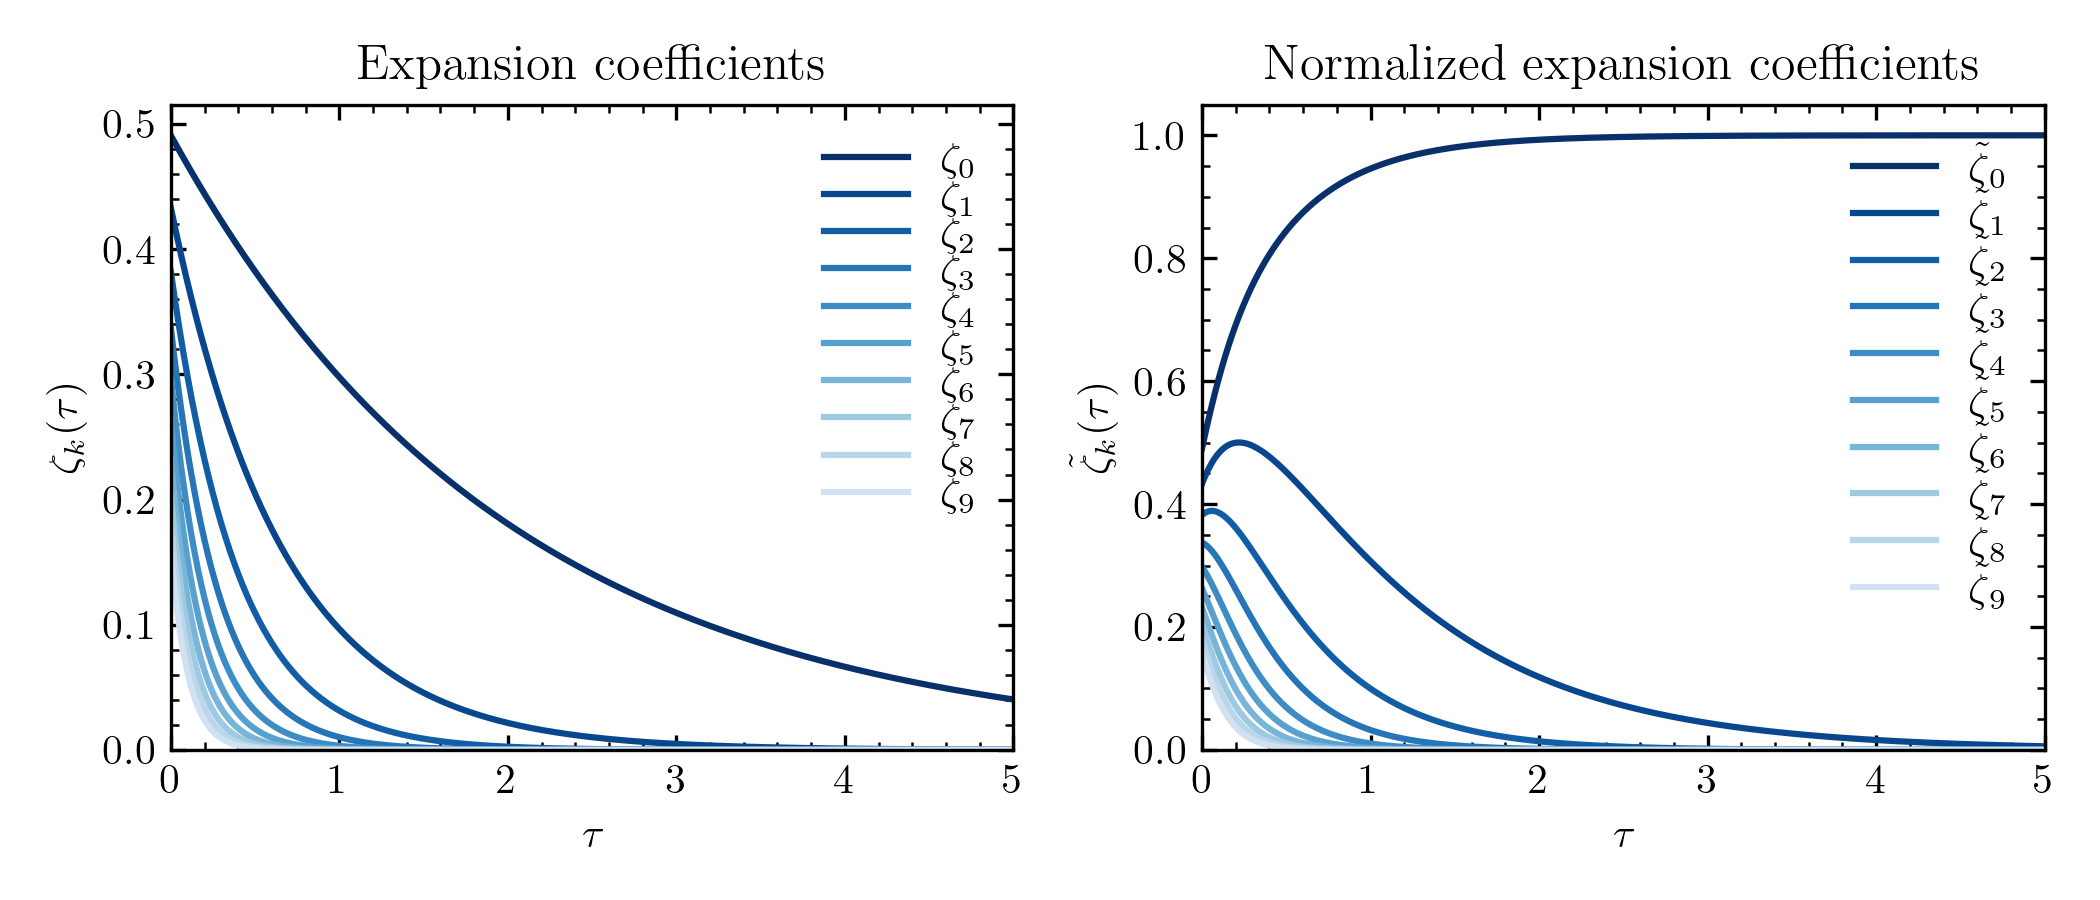
\includegraphics[width=0.9\linewidth]{scriptum/obrazky/itqd/itqd1.png}
    \caption{The time-dependent expansion coefficients of the wave function $\zeta_k(\tau) = \langle \phi_k | \psi(\tau) \rangle$ (left) and expansion coefficients of its normalized counterpart $\Tilde{\zeta}_k(\tau) = \langle \phi_k | \Tilde{\psi}(\tau) \rangle$ (right) for a harmonic oscillator. All the coefficients $\zeta_k$ decay exponentially, yet some faster and some slower depending on their energy $E_k$. The normalized expansion coefficients $\Tilde{\zeta}_k$ show that the lowest-state contribution is increasing while the other states contribute less in time. The initial increase in $\Tilde{\zeta}_1$ is given by the other higer-energy states which decay much faster but once they decay, $\Tilde{\zeta}_1$ also starts decreasing.}
    \label{fig:itqd1}
\end{figure}


So far we have shown that the imaginary-time dynamics can help us to optimize the lowest-energy state, but what if we also want higher states? In principle, we can optimize an arbitrary state with imaginary quantum dynamics. The correct statement of what we have derive would rather be that the imaginary-time dynamics converges to the lowest-energy state that contributes to the initial wave function $\psi(x,0)$. If the ground state expansion coefficient $c_0$ is equal to 0, the ground-state contribution will be zero for all times and we will never acquire the ground state wave function. We can only acquire a wave function of the lowest-energy state contributing to the initial wave function, i.e., with a nonzero expansion coefficient at the beginning of the dynamics.

This realization gives us a recipe to calculate higher-energy states: we need to construct the initial wave function such that it has zero contribution from all the lower-energy states. Thus, we must project out these states from the initial wave function. Taking the example of the first excited state, we need to first run the imaginary time dynamics and optimize $\phi_0$. Then, we need to project out this ground state from the initial wave function $\psi(x,0)$, creating a new initial wave function
\begin{equation}
    \psi_1(x,0) = \psi(x,0) - c_0 \phi_0(x) = \sum_{k=0}^\infty c_k \phi_k(x) - c_0 \phi_0(x) = \sum_{k=1}^\infty c_k \phi_k(x) \, ,
\end{equation}
which needs to be renormalized such that $\sum_{k=1}^\infty |c_k|^2 = 1$. Applying $\hat{U}_\mathrm{IT}$ to $\psi_1(x,0)$ then leads to $\phi_1(x)$ we wanted to optimize:
\begin{equation}
    \lim_{\tau\to\infty} \Tilde{\psi_1}(x,\tau) = \phi_1(x) \, .
\end{equation}
Hence, if we want to optimize an arbitrary eigenstate, we first need to optimize all the lower-energy states and project them out from the initial wave function. In this manner, we gradually acquire the eigenstates from the bottom.

In the end, let us return and comment on the imaginary time. What is it and how should we image a propagation in imaginary time? The concept of imaginary time seems elusive since no one has ever seen a watch measuring imaginary time. Still, the concept of imaginary time is not new in physics and appears, for example, in general relativity and cosmology, yet the concept is definitely not easy to grasp. The imaginary time often appears in equations as a mathematical 'trick' that allows us to reformulate equations into a better form. Although there are attempts to interpret the imaginary time, they still remain in the realm of speculations. If the imaginary time creates confusion in the reader, we recommend to view it rather as a mathematical construct that allows us to create a new operator with desired properties. The operator serves as a tool to obtain eigenstates and we do not need to attribute it any physical meaning, despite having a clear connection to dynamics


\section{Numerical implementation}

Numerical implementation of the imaginary-time quantum dynamics builds on the real-time quantum dynamics, where the imaginary unit needs to be removed from the exponentials in the propagator. The propagation in time is otherwise the same except for two minor additions to the code.

First, we need to renormalize the propagated wave function $\psi(x,\tau)$ at every time step since we are interested in the normalized $\Tilde{\psi}(x,t)$. Normalization is also important to make the calculation numerically stable. We could propagate $\psi$ without normalization and normalize it at the end, yet we would soon run into numerical issues with the exponential decay or increase in the norm. Plus we still need the norm to evaluate the energy at every step. The renormalization is a simple one-line modification after the propagation step.

The second addition to the code concerns the calculation of excited states (states above the ground state). As we have shown in the previous section, the imaginary-time dynamics converge to the lowest state in the expansion of $\psi(x,0)$. Thus, the calculation of an arbitrary state $l$ requires projecting out all states $j$ below $l$ from the initial wave function. Note that renormalization is necessary after the removal of the lower states. Therefore, the renormalization described in the previous paragraph is convenient after this step. 
% The procedure is schematically highlighted in the following scheme:
% \begin{equation}
    % \psi(x,0) \rightarrow \psi^\prime_l(x,0) = \psi(x,0) - \sum_{j<l}\langle \phi_j | \psi(x,0) \rangle \rightarrow \psi_l(x,0) = \frac{\psi^\prime_l(x,0)}{\langle \psi^\prime_l(x,0) | \psi^\prime_l(x,0) \rangle^2} 
% \end{equation}
% \textbf{Consider splitting in to equations.}

While this projection of the initial wave function would be in theory sufficient only at the beginning, the numerical precision of a computer alter the wave function a bit at every step which can create a tiny contribution of the lower states. These contributions are at the order of a computer precision, i.e., very small, but they can become important at longer dynamics since they are enhanced exponentially. Hence, the projecting out should be done also during the dynamics. The simplest is to project out at every time step but it is possible to optimize the algorithm and project out with some frequency.

We conclude with a remark not related to the implementation. If the eigenstate we seek has $c_k=0$, we cannot optimize it with imaginary-time dynamics. The initial wave function $\psi(x,0)$ should always be selected such that the coefficient of the desired state $k$ is not zero. This is similar to the previous chapter about the autocorrelation function and we can use the same principles. 


\section{Code}

\lstset{style=mystyle}
\lstinputlisting[caption=Incomplete code for the imaginary-time quantum dynamics.,language=Python]{codes/exercises/it_quantum_dynamics.py}

\section{Applications}

\subsection*{Exercise: Harmonic oscillator}

The spectrum of a harmonic oscillator was already calculated in the previous chapter as \acrlong{ft} of the autocorrelation function. The same spectrum can be also obtained by the imaginary-time quantum dynamics. Furthermore, the imaginary time dynamics also provide wave functions of the eigenstates which are not available from the autocorrelation function. In this Exercise, we will try to calculate the energies and wave functions of the harmonic oscillator and compare them to the exact analytic results, serving as a validation of the code.

\paragraph{Assignment:} Set up a harmonic oscillator from Eq.~\eqref{eq:qdho} and an initial Gaussian wave packet from Eq.~\eqref{eq:qdgauss} with the following parameters: $m=1$~a.u., $\omega=0.1$~a.u., $x_0=6$~a.u., $p_0=0$~a.u. and $\alpha_0 = 0.3$. Propagate the wave packet in imaginary time to optimise the lowest ten states of the harmonic oscillator. Compare the energies and wave functions with analytic results.

\subsection*{Exercise: Double-well potential}

The double-well potential is one of the simplest model potentials for chemical reactions with an activation barrier. In realistic scenarios, such reactions often exhibit an asymmetry between the two wells, where one minimum is energetically lower than the other. The asymmetric double-well potential can be described by the following expression:
\begin{equation*}
    V(x) = \frac{1}{2}m\omega^2(x^4 - x^2) + \xi x \, .
\end{equation*}
where $m$ is the mass, $\omega$ is the harmonic frequency, and $\xi$ is the asymmetry parameter. This exercise explores the behaviour of wave functions in such a potential, focusing on the number of quantum states localized in the wells and the extent of tunnelling between them.

\paragraph{Assignment:} Prepare a double well potential with parameters $m=20$~a.u., $\omega=2$~a.u. and $\xi=0.5$~a.u. First, initialize the wave function such that it spans both wells and optimize at least fifteen states. 
How many states are located only in one well? Is there a state with energy below the barrier that tunnels between the wells? Can you describe the difference between states below the activation barrier and above it?
Then, initialize the dynamics with a wave function in the form of Eq.~\eqref{eq:qdgauss} and parameters $x_0=-0.90$~a.u., $p_0=0$~a.u. and $\alpha_0 = 2m\omega$~a.u., i.e. the initial wave function will be located in the left well. Observe how the wave function first converges to states in the left well before the lower energy contributions from the right well take over. Can you explain the behaviour?

%%%%%%%%%%%%%%%%%%%%%%%%%% OTHER EXERCISE %%%%%%%%%%%%%%%%%%%%%%%%%%%
%%%%%%%%%%%%%%%%%%%%%%%%%% TO BE FINISHED %%%%%%%%%%%%%%%%%%%%%%%%%%%

% \subsection*{*Exercise: Morse potential}

% \begin{equation*}
%     V(x) = D_e \left(1 - \e^{-a(x-x_e)}\right)^2 \, .
% \end{equation*}

% \paragraph{Assignment:} Text

% \subsection*{*Exercise: OH radical}

% % Maybe OH radical? What temperature would lead to Boltzmann population of the most loosely bound state to be 0.2%?

% \paragraph{Assignment:} Text

% \chapter{Nonadiabatic quantum dynamics}
% \label{kap:nonad}
% % Up to this point, we have taken the time-independent perspective on quantum mechanics, focusing on methods for calculating stationary states of electrons in molecules. In this chapter, we shift to time-dependent quantum mechanics and look at the time evolution of quantum systems. We will focus on simple low-dimensional models and introduce a simple numerical scheme suitable for wave function propagation. The power of simple low-dimensional models resides in the conceptual understanding of time evolution in quantum mechanics: they allow us to examine dynamics such as interference of two wave packets, tunnelling through energy barriers, or reflection of the wave packet on boundaries.

\section{Theoretical background}
\label{sec:qdtheoback}

The time evolution in quantum mechanics is governed by the \acrfull{tdse},
\begin{equation}
    i\hbar\frac{\dd\psi(x,t)}{\dd t} = \hat{H}(x)\psi(x,t) \, ,
    \label{eq:tdse}
\end{equation}
where $i$ is the imaginary unit, $\hbar$ is the reduced Planck constant, $\psi$ is the wave function, $\hat{H}$ is the Hamiltonian, $t$ is time and $x$ represents the position of a quantum particle, such as an electron, proton, or any other particle. The solution of the \acrshort{tdse} can be in general written as
\begin{equation}
    \psi(x,t) = \hat{U}(t)\psi(x,0) \, .
    \label{eq:U}
\end{equation}
The operator $\hat{U}$ is called a \textit{propagator} or \textit{time evolution operator}. Application of the propagator to a wave function is equivalent to evolving the wave function from time 0 to time t. The knowledge of the evolution operator is, therefore, elementary for a description of dynamics in quantum systems.

The propagator is easy to find if the Hamiltonian $\hat{H}$ does not depend on time. Then, we can formally write a solution of equation~\eqref{eq:tdse} in the following form:
\begin{equation}
    \psi(x,t) = \e^{-\frac{i}{\hbar}\hat{H}(x)t} \psi(x,0)\, .
    \label{eq:tdse2}
\end{equation}
Notice that the result resembles the separation of variables for differential equations, only for a equation with operators. Considering the Hamiltonian to be time-independent restricts the validity of equation~\eqref{eq:tdse2} only for systems without any time-dependent interaction such as oscillating electromagnetic field (radiation), collisions between particles, etc. The solution for time-dependent Hamiltonian is somewhat more complicated and will be omitted here.

Comparing equations~\eqref{eq:tdse2} and \eqref{eq:U}, we see that the evolution operator has a simple form of an exponential of the Hamiltonian,
\begin{equation}
    \hat{U}(t) = \e^{-\frac{i}{\hbar}\hat{H}(x)t} \, .
    \label{eq:U1}
\end{equation}
Formally, we now have a propagator containing all information about the time evolution of the system and we can propagate the wave function to an arbitrary time $t$. While this works well on paper, analytical evaluation of the propagator is in practice not a straightforward task for most Hamiltonians. The hindrance lies in the evaluation of the exponential in equation~\eqref{eq:U1}.

Let us briefly discuss why analytic evaluation of the exponential of Hamiltonian is a cumbersome task. The exponential of an operator is defined through its Taylor series as
\begin{equation}
    \e^{\hat{A}} = \sum_{l=0}^\infty \frac{\hat{A}^l}{l!} \, ,
\end{equation}
where $\hat{A}$ is and arbitrary operator. In our case, $\hat{A} = -\frac{i}{\hbar}\hat{H}(x)t$ which leads to the following relation:
\begin{equation}
    \hat{U}(t) = \sum_{l=0}^\infty \frac{\hat{H}^l}{l!} \left( -\frac{i}{\hbar} t\right)^l \, .
    \label{eq:U2}
\end{equation}
Considering the Hamiltonian in the standard form,
\begin{equation}
    \hat{H}(x) = \hat{T} + \hat{V}(x) = -\frac{\hbar^2}{2m}\frac{\dd^2}{\dd x^2} + V(x)\, ,
    \label{eq:Ham1}
\end{equation}
where $\hat{T}$ represents the kinetic energy operator, $\hat{V}$ stands for the potential energy operator and $m$ is the particle mass, the propagator becomes:
\begin{equation}
    \hat{U}(t) = \sum_{l=0}^\infty \frac{(\hat{T}+\hat{V})^l}{l!} \left( -\frac{i}{\hbar} t\right)^l \, .
    \label{eq:U3}
\end{equation}
Calculating this propagator requires computing an infinite series of powers of the Hamiltonian, further complicated by the fact that $\hat{T}$ and $\hat{V}$ do not commute and the exponential cannot be factorized. This makes direct evaluation infeasible for most of the potential.

Thus, analytical solutions of the \acrshort{tdse} are used only in model systems, usually when the complete basis of the respective Hilbert space is known. Instead, most time-dependent problems are solved numerically where arbitrary Hamiltonians are possible. 

\section{Numerical solution}

Systems of chemical interest span, in general, an infinite Hilbert space. In other words, an infinite number of orthogonal basis functions are required to fully represent the wave function of such a system. However, any computer can only handle a finite basis set, since computer memory is finite, and often even quite limited. Thus, in any numerical implementation of quantum mechanics, we work in a truncated basis set. This basis truncation is the first and fundamental source of error for any computer simulation. There are other sources of error due to the numeric schemes employed, e.g. trapezoid rule for integration, or due to a finite time step in our propagation. While these sources of error can be eliminated by improving our numeric schemes or the time step, the truncation error will be always present and dependent on how much we truncated our basis.
% consider reformulating the fundamental error and other errors

In this text, we will represent the system on a grid of discrete points, a natural representation for a computer. These grid points (we can think of them as a set of Dirac $\delta$-distributions) form our truncated basis set commonly referred to as a \textit{pseudospectral} basis. 
In the following, we will explain how to work with such a representation, including how to evaluate the action of an operator and calculate the expectation value. In the end, the flow of the text will lead us to the evolution operator $\hat{U}(t)$ and techniques for efficient propagation of the wave function.

\subsection{Representing wave function on a grid: the \textit{pseudospectral} basis}

As stated above we will work in a truncated \textit{pseudospectral} basis and represent the system with a set of $N$ discrete points. Since we work as usual in chemistry in the position representation, we start with discretizing the position coordinate $x$ and replacing it by a set of points:
\begin{align}
    x &\rightarrow \{x_0, x_1, x_2, \dots, x_N\} \, .
\end{align}
It is convenient for numerical applications to make the grid equidistant, meaning that the distance between any two neighbouring grid points, $\Delta x = x_i - x_{i-1}$, remains constant. 

Next, we express the wave function $\psi$ on this grid by evaluating it at each grid point $x_i$, giving:
\begin{align}
    \psi(x,t) &\rightarrow \{\psi(x_0,t), \psi(x_1,t), \psi(x_2,t), \dots, \psi(x_N,t)\} =  \{\psi_{0,t}, \psi_{1,t}, \psi_{2,t}, \dots, \psi_{N,t}\} \, .
\end{align}
We have now two indexes of $\psi$: the grid point index $i$ and time index $t$. Further in the text, we will drop the index $t$ to simplify the notation unless $\psi$ in two different times will appear in the equation.

Having the wave function defined on a grid, the next step is to compute its norm. In the position representation, the norm is an integral of $\psi^*\psi$ over the position $x$, which can be numerically realized for example by the trapezoidal rule:
\begin{equation}
    \langle \psi(x,t) | \psi(x,t) \rangle = \int_{-\infty}^\infty \psi^*(x,t)\psi(x,t) \dd x = \sum_{j=1}^N \frac{\psi^*_{j-1}\psi_{j-1} + \psi^*_{j}\psi_{j}}{2} \Delta x \, .
\end{equation}
While the trapezoidal rule is a simple and commonly used method, more accurate numerical integration schemes can be employed to reduce integration errors, though these may come at the cost of increased computational effort.

With the wave function defined, our attention now turns to operators: how to represent them and how to apply them. We will start with operators dependent only on the position $x$ since they are simple to represent on the grid. Take the potential energy operator $V(x)$ which can be represented on the grid similarly to the wave function as
\begin{align}
    V(x) &\rightarrow \{V(x_0), V(x_1), V(x_2), \dots, V(x_N)\} = \{V_0, V_1, V_2, \dots, V_N\} \, .
\end{align}
Now, applying the potential energy operator to the wave function reduces to a simple multiplication of the discretized operator and wave function as 
\begin{align}
    \hat{V}\psi &\rightarrow \{V_0 \psi_0, V_1 \psi_1, V_2 \psi_2, \dots, V_N \psi_N\} \, .
\end{align}
The expectation value of the potential energy in analogy with the norm using the trapezoid rule: 
\begin{equation}
    \langle \psi(x,t) | \hat{V} | \psi(x,t) \rangle = \int_{-\infty}^\infty \psi^*(x,t)V(x)\psi(x,t) \dd x = \sum_{j=1}^N \frac{V_{j-1}\psi^*_{j-1}\psi_{j-1} + V_{j}\psi^*_{j}\psi_{j}}{2} \Delta x
\end{equation}
Any operator that depends only on the position $x$ can be represented on the grid similarly to $\hat{V}$ and the expectation values are then evaluated in the same manner as above.
However, operators that depend on momentum $\hat{p}$ require a more complex treatment, as they involve derivatives, which cannot be directly represented on the grid in the same straightforward manner.


\subsection{Applying the kinetic energy operator: the Fourier method}

% better structure: first show how to transfer between reps and then how we use it to evaluate

To evaluate the action of the kinetic energy operator, or any other operator depending on momentum, it is convenient to switch to a basis where the action of momentum operator $\hat{p}$ is a simple multiplication. Such basis is the basis of the free particle states $\e^{ikx}$, the so-called $k$-space or momentum space since $p = \hbar k$. The wave function represented in the $k$-space can be obtained by \acrfull{ift} $\mathcal{F}^{-1}$ as
\begin{align}
    \psi(k,t) = \mathcal{F}^{-1}[\psi(x,t)] =\int_{-\infty}^\infty \psi(x,t) \e^{ikx}\dd x \, .
\end{align}
Performing the \acrshort{ift} on a computer is a routine task and allows us to easily transfer between the position representation $\psi(x,t)$ and momentum representation $\psi(k,t)$.

The action of the kinetic operator on the wave function is cumbersome to evaluate numerically in the position space due to the derivatives, but it is simple in the $k$-space using the \acrshort{ift}:
\begin{align}
    \mathcal{F}^{-1}[\hat{T}\psi(x,t)] &= \mathcal{F}^{-1}\left[-\frac{\hbar^2}{2m}\frac{\dd^2 \psi(x,t)}{\dd x^2}\right] = -\frac{\hbar^2}{2m} \int_{-\infty}^\infty \frac{\dd^2 \psi(x,t)}{\dd x^2}  \e^{ikx}\dd x \stackrel{p.p.}{=} \frac{\hbar^2}{2m} i k \int_{-\infty}^\infty \frac{\dd \psi(x,t)}{\dd x} \e^{ikx}\dd x \notag \\
    &\stackrel{p.p.}{=} - i^2 \frac{\hbar^2}{2m} k^2 \int_{-\infty}^\infty \psi(x,t) \e^{ikx}\dd x = \frac{\hbar^2 k^2}{2m} \psi(k,t) \, .
    \label{eq:qdftkspace}
\end{align}
where $p.p.$ signifies integration \textit{per partes}. The result of $\hat{T}\psi$ in the $k$-space is very straightforward, just multiply $\psi(k,t)$ by the kinetic energy $\frac{\hbar^2 k^2}{2m}$.

However, we are interested in the action of $\hat{T}$ in the position space since we work on our $x$-grid. This is easily achieved by evaluating the action of $\hat{T}$ in the $k$-space, as we showed in Eq.~\eqref{eq:qdftkspace}, and then transforming the result back to the position representation with the \acrfull{ft} $\mathcal{F}$ as
\begin{align}
    \hat{T}\psi(x,t) &= \mathcal{F}\left[\frac{\hbar^2 k^2}{2m} \psi(k,t)\right] \, .
\end{align}
Once again, \acrshort{ft} is a routine operation performed on computers.

Let us now summarize the evaluation of $\hat{T}\psi(x,t)$. First, the wave function $\psi(x,t)$ has to be \acrshort{ift} to the momentum representation $\psi(k,t)$. Then, the action of $\hat{T}$ on $\psi(k,t)$ is evaluated by simply multiplying it by $\frac{\hbar^2 k^2}{2m}$. Finally, the \acrshort{ft} is applied to $\frac{\hbar^2 k^2}{2m} \psi(k,t)$ transforming it back to the position space. The whole procedure is depicted in the following scheme:
\begin{equation}
    \psi(x,t) \stackrel{\mathrm{IFT}}{\longrightarrow} \psi(k,t) \longrightarrow \frac{\hbar^2 k^2}{2m} \psi(k,t) \stackrel{\mathrm{FT}}{\longrightarrow} \hat{T}\psi(x,t) \, .
\end{equation}

\subsection{The propagator and the Split-operator technique}

As we discussed in section~\ref{sec:qdtheoback}, evaluating the propagator is strenuous due to its exponential structure and the non-commutativity of the potential and kinetic operators. The non-commutativity is the major issue for us as it prevents us from factorizing the propagator as
\begin{equation}
    \e^{-\frac{i}{\hbar}\hat{H}(x)\Delta t} \neq \e^{-\frac{i}{\hbar}V(x)t}\e^{-\frac{i}{\hbar}\hat{T}(x)t}\, .
\end{equation}
If we could factorize the propagator as above, we could evaluate the exponential of $\hat{V}$ (in the position representation) and the exponential of $\hat{T}$ (in the momentum representation) separately. However, the non-commutativity of $\hat{V}$ and $\hat{T}$ does not allow for such factorization.

A way to deal with this problem is to split the propagator into a series of $n$ short-time propagator
\begin{equation}
    \hat{U}(t) = \e^{-\frac{i}{\hbar}\hat{H}(x)t} = \e^{-\frac{i}{\hbar}\hat{H}(x)\Delta t} \e^{-\frac{i}{\hbar}\hat{H}(x)\Delta t} \cdots \e^{-\frac{i}{\hbar}\hat{H}(x)\Delta t} \, ,
    \label{eq:U4}
\end{equation}
where $\Delta t$ is a fixed time step. Now, each individual short-time propagator acts on the wave function and causes a small alteration (understand short-time propagation). This operator can be approximated in the following way
\begin{equation}
    \e^{-\frac{i}{\hbar}\hat{H}(x)\Delta t} = \e^{-\frac{i}{\hbar}V(x)\Delta t/2}\e^{-\frac{i}{\hbar}\hat{T}(x)\Delta t}\e^{-\frac{i}{\hbar}\hat{V}(x)\Delta t/2} + \mathcal{O}(\Delta t^3) \, ,
\end{equation}
where we symmetrically factorized the exponential of $\hat{H}$ into separate exponentials of $\hat{V}$ and $\hat{T}$. The factorization here is possible only if the time step $\Delta t$ is short since the error behaves as $\Delta t^3$. 

These exponentials now need to be evaluated. While the exponential of the potential energy is simply evaluated on the grid and multiplied by the wave function, the exponential of the kinetic energy operator must be evaluated using the Fourier method introduced in the previous subsection as
\begin{equation}
    \psi(x,t) \stackrel{\mathrm{IFT}}{\longrightarrow} \psi(k,t) \longrightarrow \e^{\frac{i}{\hbar} \frac{\hbar^2 k^2}{2m} t} \psi(k,t) \stackrel{\mathrm{FT}}{\longrightarrow} \e^{-\frac{i}{\hbar} \hat{T} t}\psi(x,t) \, .
\end{equation}
The whole propagation is then done in a series of short time steps $\Delta t$. At each time step, the wave function is first propagated by a half step in potential energy, then a full step in kinetic energy and finally again a half step in potential energy. 

\section{Code}

The numerical procedure for quantum dynamics described above can be readily implemented in Python or another suitable programming language. Let us start with a few short notes regarding a Python implementation. We will exploit the \python{numpy} library (imported as \python{np}). The \acrlong{ft} can be conveniently performed as
\begin{lstlisting}[language=Python, style=mystyle2]
np.fft.fft(psi, norm="ortho")
\end{lstlisting}
with \python{psi} being the wave function. Setting \python{norm="ortho"} employs the orthogonal norm. While we could use a different norm, we need to make sure we use the same norm for the \acrshort{ift} to ensure unitarity. The corresponding $k$-space is generated with
\begin{lstlisting}[language=Python, style=mystyle2]
2*np.pi*np.fft.fftfreq(ngrid, d=dx)
\end{lstlisting}
where we supply the number of grid points (\python{ngrid}) and the distance between two neighbouring points (\python{dx}). The \acrlong{ift} can be calculated similarly: 
\begin{lstlisting}[language=Python, style=mystyle2]
f = np.fft.ifft(psi_k, norm="ortho")
\end{lstlisting}

The integration can be achieved with the trapezoidal rule in Python by selecting
\begin{lstlisting}[language=Python, style=mystyle2]
np.trapz(y=np.conjugate(psi)*psi, x=x)
\end{lstlisting}
The trapezoidal rule is used here to compute the normalization of the wave function or to calculate expectation values by integrating over space.

Since the wave function is a complex function, we will also need to work with complex numbers in Python. Python works with \python{j} as the complex unit. The corresponding data type is called \python{complex}. Thus, creating an initial wave function can look like 
\begin{lstlisting}[language=Python, style=mystyle2]
psi = (2*alpha/np.pi)**0.25*np.exp(-alpha*(x-x0)**2+1j*p0*(x-x0), dtype=complex)
\end{lstlisting}

Follows the incomplete code for quantum dynamics with empty gaps where the students are supposed to define operators and propagate the wave function according to the method description above. The code is prepared in atomic units where $\hbar=1$~a.u. and requires all the input parameters also in atomic units. The span of the $x$-axis, defined by \python{xmin} and \python{xmax}, should be large enough to contain the entire wave packet during propagation and is set for each simulation individually based on the system. The wave packet should never reach the boundaries defined by \python{xmin} and \python{xmax}. The number of grid points should be sufficiently big to represent the wave function. A few hundred to a few thousand grid points should suffice for simple dynamics. The time step \python{dt} should be significantly smaller than the time scale on which the wave packet evolves, which depends on its mass and potential. Always make sure the energy and norm are conserved during dynamics as they are indicators of a spurious propagation. Decreasing \python{dt} and increasing \python{ngrid} should always improve both energy and norm conservation. 

\lstset{style=mystyle}
\lstinputlisting[caption=Incomplete code for quantum dynamics in real time.,language=Python]{codes/exercises/rt_quantum_dynamics.py}

\section{Applications}

\subsection*{Exercise: Squeezed and coherent states of harmonic oscillator}

The harmonic oscillator and Gaussian wave packet are some of the most important objects in quantum mechanics. While the harmonic oscillator is used as the first approximation to many bound Hamiltonians, the Gaussian wave packet is a commonly used basis function in quantum dynamics. There is a special relationship between them: any initial Gaussian wave function, $\psi(x,0)$, propagated in quadratic potential remains Gaussian throughout its evolution. In other words, a Gaussian wave packet evolving in a harmonic oscillator will retain its Gaussian form, with only its position, momentum, and width changing over time.

Gaussian wave packets evolving in harmonic oscillators can be classified into two groups: \textit{coherent} and \textit{squeezed} states. The \textit{coherent} states are characterized by a constant width of the Gaussian during the dynamics, meaning the wave packet preserves its shape while its position and momentum vary. Contrarily, if the Gaussian spreads and contracts (or contracts and spreads) during the dynamics, it is referred to as a \textit{squeezed} state.

In this exercise, we will explore the properties of \textit{coherent} and \textit{squeezed} states. We define the initial Gaussian wave packet as
\begin{equation}
    \psi(x,0) = \left(\frac{2\alpha_0}{\pi}\right)^{\frac{1}{4}} \e^{-\alpha_0(x-x_0)^2 +\frac{i}{\hbar}p_0(x-x_0)} \, ,
    \label{eq:qdgauss}
\end{equation}
where $x_0$ and $p_0$ refer to the initial mean position and momentum of the Gaussian, and $\alpha_0$ is the initial Gaussian width. The potential for harmonic oscillator takes the following form:
\begin{equation}
    V = \frac{1}{2}m\omega^2x^2 \, .
    \label{eq:qdho}
\end{equation}
The aim is to determine the Gaussian width $\alpha_0$ corresponding to a \textit{coherent} state by trying different values of $\alpha_0$.

\paragraph{Assignment:} Set up the harmonic oscillator from Eq.~\eqref{eq:qdho} and initial Gaussian wave packet from Eq~\eqref{eq:qdgauss} with the following parameters: $m=20$~a.u., $\omega=2$~a.u., $x_0=0$~a.u. and $p_0=20$~a.u. Set up a trial $\alpha_0$ (Hint: try $\alpha_0$ as a factor of $\frac{m\omega}{\hbar}$). Propagate the wave packet for several oscillation and visualize it. If the wave packet contracts in the center of the potential, increase $\alpha_0$. If the wave packet spreads, decrease $\alpha_0$ to approach a coherent state. Iterate that procedure until you find the value of $\alpha_0$ corresponding to the \textit{coherent} state. 

\subsection*{Exercise: Ehrenfest's theorems in harmonic oscillator}

Ehrenfest's theorems provide a connection between classical and quantum dynamics. They represent equations of motion for expectation values of position $\braket{x}$ and momenta $\braket{p}$. For a harmonic oscillator, Ehrenfest's theorems take the following form:
\begin{align*}
    \frac{\dd \braket{x}}{\dd t} &= \frac{\braket{p}}{m} \\
    \frac{\dd \braket{p}}{\dd t} &= -\frac{\dd V(\braket{x})}{\dd \braket{x}} \, .
\end{align*}
These equations are equivalent to the classical Newton's equations of motion, only for expectation values of position $\braket{x}$ and momenta $\braket{p}$ instead of classical $x$ and $p$. This exercise aims to verify that the relations above hold true for harmonic oscillator and $\braket{x}$ and $\braket{p}$ follow a classical trajectory. Equally, one can consider a anharmonic potential, e.g. Morse potential, and show that the relations above are not exact.

\paragraph{Assignment:} Choose an arbitrary initial wave function and harmonic potential. Propagate the wave function for several oscillations and calculate the expectation values of position $\braket{x}$ and momenta $\braket{p}$ over time. Compare the calculated values with a classical trajectory with the same initial conditions. The classical trajectory can be obtained by solving Newton's equations of motion. Repeat the same procedure for an anharmonic Morse potential and show that the relation above does not hold. Note that you will probably need to calculate the classical trajectory numerically, for example by a Verlet method.


\subsection*{Exercise: Tunnelling in a double-well potential}

Tunnelling is an ubiquitous phenomenon in quantum world which is difficult to grasp from classical perspective. It plays an important role in chemistry where light atoms, such as protons, can tunnel through energy barriers causing energetically forbidden reactions. This exercise focuses at tunnelling through a double-well potential,
\begin{equation*}
    V = \frac{1}{2}m\omega^2(x^4 - x^2) \, .
\end{equation*}
The wave function will be initiated at the edge of the left well, which will send it to the right towards the barrier. Two scenarios are possible. First, the energy of the wave packet is below the barrier. Then, no density should be observed at the other well from classical perspective. Thus, any density observed in the right well is due to quantum tunnelling. In the second scenario, the wave packet energy is above the barrier. Classical particles would then transfer to the other well without loss of density, yet this is again not true for the quantum world. The wave packet partially reflects on the barrier and some density remains in the original well.

To assess the amount of density transferred to the right well, we devise a coefficient $\kappa$ defined as
\begin{equation*}
    \kappa(t) = \int_0^{\infty} \psi^*(x,t) \psi(x,t) \dd x \,.
\end{equation*}
The value of $\kappa$ will tell us how big portion of the density is located in the right well, i.e. about the tunnelling efficiency in the first scenario and reflective strength in the second scenario.

\paragraph{Assignment:} Prepare a double well potential with parameters $m=20$~a.u. and $\omega=2$~a.u. First, initialize the dynamics with a wave function in form of Eq.~\eqref{eq:qdgauss} with parameters $x_0=-0.90$~a.u., $p_0=0$~a.u. and $\alpha_0 = 2m\omega$~a.u. (the energy of the wave packet should be below the barrier). Second, initialize the dynamics with parameters $x_0=-0.95$~a.u., $p_0=8$~a.u. and $\alpha_0=2m\omega$~a.u. (the energy should be above the barrier). Calculate the parameter $\kappa$ for both scenarios and compare them with your expectations base on classical physics. Analyse the dynamics also visually by plotting the density in time. Con you identify interferences of the reflected and tunnelled wave packets?

\subsection*{Exercise: Heisenberg's uncertainity relations}

The uncertainty principle developed by Werner Heisenberg is one of the corner stones of quantum mechanics. It states that
\begin{equation*}
    \Delta x \Delta p \ge \frac{\hbar}{2} \, , 
\end{equation*}
where
\begin{align*}
    \Delta x &= \braket{x^2} - \braket{x}^2 = \bra{\psi(x, t)}x^2\ket{\psi(x,t)} -  \bra{\psi(x, t)}x\ket{\psi(x,t)}^2\\
    \Delta p &= \braket{p^2} - \braket{p}^2 = \bra{\psi(x, t)}\hat{p}^2\ket{\psi(x,t)} -  \bra{\psi(x, t)}\hat{p}\ket{\psi(x,t)}^2 \, .
\end{align*}
However, the uncertainty principle states only the lower boundary for $\Delta x \Delta p$ and does not tell us if it remains constant, rises or oscillates throughout the time evolution. The goal of this exercise is to empirically estimate whether the product $ \Delta x \Delta p$ remains constant in time or not. If not, how does it behave?

\paragraph{Assignment:} Evolve an arbitrary initial Gaussian wave packet in a harmonic oscillator and estimate the product $\Delta x \Delta p$ in time during the dynamics. Try the same also for a Morse potential and a double-well potential. Estimate how the product $\Delta x \Delta p$ behaves and if the behaviour differs between the potentials.

% \chapter{Wigner transformation}
% \label{kap:wigner}
% % \input{scriptum/texty/wigner}

% \chapter{Bohmian dynamics}
% \label{kap:bohm}
% % Up to this point, we have taken the time-independent perspective on quantum mechanics, focusing on methods for calculating stationary states of electrons in molecules. In this chapter, we shift to time-dependent quantum mechanics and look at the time evolution of quantum systems. We will focus on simple low-dimensional models and introduce a simple numerical scheme suitable for wave function propagation. The power of simple low-dimensional models resides in the conceptual understanding of time evolution in quantum mechanics: they allow us to examine dynamics such as interference of two wave packets, tunnelling through energy barriers, or reflection of the wave packet on boundaries.

\section{Theoretical background}
\label{sec:qdtheoback}

The time evolution in quantum mechanics is governed by the \acrfull{tdse},
\begin{equation}
    i\hbar\frac{\dd\psi(x,t)}{\dd t} = \hat{H}(x)\psi(x,t) \, ,
    \label{eq:tdse}
\end{equation}
where $i$ is the imaginary unit, $\hbar$ is the reduced Planck constant, $\psi$ is the wave function, $\hat{H}$ is the Hamiltonian, $t$ is time and $x$ represents the position of a quantum particle, such as an electron, proton, or any other particle. The solution of the \acrshort{tdse} can be in general written as
\begin{equation}
    \psi(x,t) = \hat{U}(t)\psi(x,0) \, .
    \label{eq:U}
\end{equation}
The operator $\hat{U}$ is called a \textit{propagator} or \textit{time evolution operator}. Application of the propagator to a wave function is equivalent to evolving the wave function from time 0 to time t. The knowledge of the evolution operator is, therefore, elementary for a description of dynamics in quantum systems.

The propagator is easy to find if the Hamiltonian $\hat{H}$ does not depend on time. Then, we can formally write a solution of equation~\eqref{eq:tdse} in the following form:
\begin{equation}
    \psi(x,t) = \e^{-\frac{i}{\hbar}\hat{H}(x)t} \psi(x,0)\, .
    \label{eq:tdse2}
\end{equation}
Notice that the result resembles the separation of variables for differential equations, only for a equation with operators. Considering the Hamiltonian to be time-independent restricts the validity of equation~\eqref{eq:tdse2} only for systems without any time-dependent interaction such as oscillating electromagnetic field (radiation), collisions between particles, etc. The solution for time-dependent Hamiltonian is somewhat more complicated and will be omitted here.

Comparing equations~\eqref{eq:tdse2} and \eqref{eq:U}, we see that the evolution operator has a simple form of an exponential of the Hamiltonian,
\begin{equation}
    \hat{U}(t) = \e^{-\frac{i}{\hbar}\hat{H}(x)t} \, .
    \label{eq:U1}
\end{equation}
Formally, we now have a propagator containing all information about the time evolution of the system and we can propagate the wave function to an arbitrary time $t$. While this works well on paper, analytical evaluation of the propagator is in practice not a straightforward task for most Hamiltonians. The hindrance lies in the evaluation of the exponential in equation~\eqref{eq:U1}.

Let us briefly discuss why analytic evaluation of the exponential of Hamiltonian is a cumbersome task. The exponential of an operator is defined through its Taylor series as
\begin{equation}
    \e^{\hat{A}} = \sum_{l=0}^\infty \frac{\hat{A}^l}{l!} \, ,
\end{equation}
where $\hat{A}$ is and arbitrary operator. In our case, $\hat{A} = -\frac{i}{\hbar}\hat{H}(x)t$ which leads to the following relation:
\begin{equation}
    \hat{U}(t) = \sum_{l=0}^\infty \frac{\hat{H}^l}{l!} \left( -\frac{i}{\hbar} t\right)^l \, .
    \label{eq:U2}
\end{equation}
Considering the Hamiltonian in the standard form,
\begin{equation}
    \hat{H}(x) = \hat{T} + \hat{V}(x) = -\frac{\hbar^2}{2m}\frac{\dd^2}{\dd x^2} + V(x)\, ,
    \label{eq:Ham1}
\end{equation}
where $\hat{T}$ represents the kinetic energy operator, $\hat{V}$ stands for the potential energy operator and $m$ is the particle mass, the propagator becomes:
\begin{equation}
    \hat{U}(t) = \sum_{l=0}^\infty \frac{(\hat{T}+\hat{V})^l}{l!} \left( -\frac{i}{\hbar} t\right)^l \, .
    \label{eq:U3}
\end{equation}
Calculating this propagator requires computing an infinite series of powers of the Hamiltonian, further complicated by the fact that $\hat{T}$ and $\hat{V}$ do not commute and the exponential cannot be factorized. This makes direct evaluation infeasible for most of the potential.

Thus, analytical solutions of the \acrshort{tdse} are used only in model systems, usually when the complete basis of the respective Hilbert space is known. Instead, most time-dependent problems are solved numerically where arbitrary Hamiltonians are possible. 

\section{Numerical solution}

Systems of chemical interest span, in general, an infinite Hilbert space. In other words, an infinite number of orthogonal basis functions are required to fully represent the wave function of such a system. However, any computer can only handle a finite basis set, since computer memory is finite, and often even quite limited. Thus, in any numerical implementation of quantum mechanics, we work in a truncated basis set. This basis truncation is the first and fundamental source of error for any computer simulation. There are other sources of error due to the numeric schemes employed, e.g. trapezoid rule for integration, or due to a finite time step in our propagation. While these sources of error can be eliminated by improving our numeric schemes or the time step, the truncation error will be always present and dependent on how much we truncated our basis.
% consider reformulating the fundamental error and other errors

In this text, we will represent the system on a grid of discrete points, a natural representation for a computer. These grid points (we can think of them as a set of Dirac $\delta$-distributions) form our truncated basis set commonly referred to as a \textit{pseudospectral} basis. 
In the following, we will explain how to work with such a representation, including how to evaluate the action of an operator and calculate the expectation value. In the end, the flow of the text will lead us to the evolution operator $\hat{U}(t)$ and techniques for efficient propagation of the wave function.

\subsection{Representing wave function on a grid: the \textit{pseudospectral} basis}

As stated above we will work in a truncated \textit{pseudospectral} basis and represent the system with a set of $N$ discrete points. Since we work as usual in chemistry in the position representation, we start with discretizing the position coordinate $x$ and replacing it by a set of points:
\begin{align}
    x &\rightarrow \{x_0, x_1, x_2, \dots, x_N\} \, .
\end{align}
It is convenient for numerical applications to make the grid equidistant, meaning that the distance between any two neighbouring grid points, $\Delta x = x_i - x_{i-1}$, remains constant. 

Next, we express the wave function $\psi$ on this grid by evaluating it at each grid point $x_i$, giving:
\begin{align}
    \psi(x,t) &\rightarrow \{\psi(x_0,t), \psi(x_1,t), \psi(x_2,t), \dots, \psi(x_N,t)\} =  \{\psi_{0,t}, \psi_{1,t}, \psi_{2,t}, \dots, \psi_{N,t}\} \, .
\end{align}
We have now two indexes of $\psi$: the grid point index $i$ and time index $t$. Further in the text, we will drop the index $t$ to simplify the notation unless $\psi$ in two different times will appear in the equation.

Having the wave function defined on a grid, the next step is to compute its norm. In the position representation, the norm is an integral of $\psi^*\psi$ over the position $x$, which can be numerically realized for example by the trapezoidal rule:
\begin{equation}
    \langle \psi(x,t) | \psi(x,t) \rangle = \int_{-\infty}^\infty \psi^*(x,t)\psi(x,t) \dd x = \sum_{j=1}^N \frac{\psi^*_{j-1}\psi_{j-1} + \psi^*_{j}\psi_{j}}{2} \Delta x \, .
\end{equation}
While the trapezoidal rule is a simple and commonly used method, more accurate numerical integration schemes can be employed to reduce integration errors, though these may come at the cost of increased computational effort.

With the wave function defined, our attention now turns to operators: how to represent them and how to apply them. We will start with operators dependent only on the position $x$ since they are simple to represent on the grid. Take the potential energy operator $V(x)$ which can be represented on the grid similarly to the wave function as
\begin{align}
    V(x) &\rightarrow \{V(x_0), V(x_1), V(x_2), \dots, V(x_N)\} = \{V_0, V_1, V_2, \dots, V_N\} \, .
\end{align}
Now, applying the potential energy operator to the wave function reduces to a simple multiplication of the discretized operator and wave function as 
\begin{align}
    \hat{V}\psi &\rightarrow \{V_0 \psi_0, V_1 \psi_1, V_2 \psi_2, \dots, V_N \psi_N\} \, .
\end{align}
The expectation value of the potential energy in analogy with the norm using the trapezoid rule: 
\begin{equation}
    \langle \psi(x,t) | \hat{V} | \psi(x,t) \rangle = \int_{-\infty}^\infty \psi^*(x,t)V(x)\psi(x,t) \dd x = \sum_{j=1}^N \frac{V_{j-1}\psi^*_{j-1}\psi_{j-1} + V_{j}\psi^*_{j}\psi_{j}}{2} \Delta x
\end{equation}
Any operator that depends only on the position $x$ can be represented on the grid similarly to $\hat{V}$ and the expectation values are then evaluated in the same manner as above.
However, operators that depend on momentum $\hat{p}$ require a more complex treatment, as they involve derivatives, which cannot be directly represented on the grid in the same straightforward manner.


\subsection{Applying the kinetic energy operator: the Fourier method}

% better structure: first show how to transfer between reps and then how we use it to evaluate

To evaluate the action of the kinetic energy operator, or any other operator depending on momentum, it is convenient to switch to a basis where the action of momentum operator $\hat{p}$ is a simple multiplication. Such basis is the basis of the free particle states $\e^{ikx}$, the so-called $k$-space or momentum space since $p = \hbar k$. The wave function represented in the $k$-space can be obtained by \acrfull{ift} $\mathcal{F}^{-1}$ as
\begin{align}
    \psi(k,t) = \mathcal{F}^{-1}[\psi(x,t)] =\int_{-\infty}^\infty \psi(x,t) \e^{ikx}\dd x \, .
\end{align}
Performing the \acrshort{ift} on a computer is a routine task and allows us to easily transfer between the position representation $\psi(x,t)$ and momentum representation $\psi(k,t)$.

The action of the kinetic operator on the wave function is cumbersome to evaluate numerically in the position space due to the derivatives, but it is simple in the $k$-space using the \acrshort{ift}:
\begin{align}
    \mathcal{F}^{-1}[\hat{T}\psi(x,t)] &= \mathcal{F}^{-1}\left[-\frac{\hbar^2}{2m}\frac{\dd^2 \psi(x,t)}{\dd x^2}\right] = -\frac{\hbar^2}{2m} \int_{-\infty}^\infty \frac{\dd^2 \psi(x,t)}{\dd x^2}  \e^{ikx}\dd x \stackrel{p.p.}{=} \frac{\hbar^2}{2m} i k \int_{-\infty}^\infty \frac{\dd \psi(x,t)}{\dd x} \e^{ikx}\dd x \notag \\
    &\stackrel{p.p.}{=} - i^2 \frac{\hbar^2}{2m} k^2 \int_{-\infty}^\infty \psi(x,t) \e^{ikx}\dd x = \frac{\hbar^2 k^2}{2m} \psi(k,t) \, .
    \label{eq:qdftkspace}
\end{align}
where $p.p.$ signifies integration \textit{per partes}. The result of $\hat{T}\psi$ in the $k$-space is very straightforward, just multiply $\psi(k,t)$ by the kinetic energy $\frac{\hbar^2 k^2}{2m}$.

However, we are interested in the action of $\hat{T}$ in the position space since we work on our $x$-grid. This is easily achieved by evaluating the action of $\hat{T}$ in the $k$-space, as we showed in Eq.~\eqref{eq:qdftkspace}, and then transforming the result back to the position representation with the \acrfull{ft} $\mathcal{F}$ as
\begin{align}
    \hat{T}\psi(x,t) &= \mathcal{F}\left[\frac{\hbar^2 k^2}{2m} \psi(k,t)\right] \, .
\end{align}
Once again, \acrshort{ft} is a routine operation performed on computers.

Let us now summarize the evaluation of $\hat{T}\psi(x,t)$. First, the wave function $\psi(x,t)$ has to be \acrshort{ift} to the momentum representation $\psi(k,t)$. Then, the action of $\hat{T}$ on $\psi(k,t)$ is evaluated by simply multiplying it by $\frac{\hbar^2 k^2}{2m}$. Finally, the \acrshort{ft} is applied to $\frac{\hbar^2 k^2}{2m} \psi(k,t)$ transforming it back to the position space. The whole procedure is depicted in the following scheme:
\begin{equation}
    \psi(x,t) \stackrel{\mathrm{IFT}}{\longrightarrow} \psi(k,t) \longrightarrow \frac{\hbar^2 k^2}{2m} \psi(k,t) \stackrel{\mathrm{FT}}{\longrightarrow} \hat{T}\psi(x,t) \, .
\end{equation}

\subsection{The propagator and the Split-operator technique}

As we discussed in section~\ref{sec:qdtheoback}, evaluating the propagator is strenuous due to its exponential structure and the non-commutativity of the potential and kinetic operators. The non-commutativity is the major issue for us as it prevents us from factorizing the propagator as
\begin{equation}
    \e^{-\frac{i}{\hbar}\hat{H}(x)\Delta t} \neq \e^{-\frac{i}{\hbar}V(x)t}\e^{-\frac{i}{\hbar}\hat{T}(x)t}\, .
\end{equation}
If we could factorize the propagator as above, we could evaluate the exponential of $\hat{V}$ (in the position representation) and the exponential of $\hat{T}$ (in the momentum representation) separately. However, the non-commutativity of $\hat{V}$ and $\hat{T}$ does not allow for such factorization.

A way to deal with this problem is to split the propagator into a series of $n$ short-time propagator
\begin{equation}
    \hat{U}(t) = \e^{-\frac{i}{\hbar}\hat{H}(x)t} = \e^{-\frac{i}{\hbar}\hat{H}(x)\Delta t} \e^{-\frac{i}{\hbar}\hat{H}(x)\Delta t} \cdots \e^{-\frac{i}{\hbar}\hat{H}(x)\Delta t} \, ,
    \label{eq:U4}
\end{equation}
where $\Delta t$ is a fixed time step. Now, each individual short-time propagator acts on the wave function and causes a small alteration (understand short-time propagation). This operator can be approximated in the following way
\begin{equation}
    \e^{-\frac{i}{\hbar}\hat{H}(x)\Delta t} = \e^{-\frac{i}{\hbar}V(x)\Delta t/2}\e^{-\frac{i}{\hbar}\hat{T}(x)\Delta t}\e^{-\frac{i}{\hbar}\hat{V}(x)\Delta t/2} + \mathcal{O}(\Delta t^3) \, ,
\end{equation}
where we symmetrically factorized the exponential of $\hat{H}$ into separate exponentials of $\hat{V}$ and $\hat{T}$. The factorization here is possible only if the time step $\Delta t$ is short since the error behaves as $\Delta t^3$. 

These exponentials now need to be evaluated. While the exponential of the potential energy is simply evaluated on the grid and multiplied by the wave function, the exponential of the kinetic energy operator must be evaluated using the Fourier method introduced in the previous subsection as
\begin{equation}
    \psi(x,t) \stackrel{\mathrm{IFT}}{\longrightarrow} \psi(k,t) \longrightarrow \e^{\frac{i}{\hbar} \frac{\hbar^2 k^2}{2m} t} \psi(k,t) \stackrel{\mathrm{FT}}{\longrightarrow} \e^{-\frac{i}{\hbar} \hat{T} t}\psi(x,t) \, .
\end{equation}
The whole propagation is then done in a series of short time steps $\Delta t$. At each time step, the wave function is first propagated by a half step in potential energy, then a full step in kinetic energy and finally again a half step in potential energy. 

\section{Code}

The numerical procedure for quantum dynamics described above can be readily implemented in Python or another suitable programming language. Let us start with a few short notes regarding a Python implementation. We will exploit the \python{numpy} library (imported as \python{np}). The \acrlong{ft} can be conveniently performed as
\begin{lstlisting}[language=Python, style=mystyle2]
np.fft.fft(psi, norm="ortho")
\end{lstlisting}
with \python{psi} being the wave function. Setting \python{norm="ortho"} employs the orthogonal norm. While we could use a different norm, we need to make sure we use the same norm for the \acrshort{ift} to ensure unitarity. The corresponding $k$-space is generated with
\begin{lstlisting}[language=Python, style=mystyle2]
2*np.pi*np.fft.fftfreq(ngrid, d=dx)
\end{lstlisting}
where we supply the number of grid points (\python{ngrid}) and the distance between two neighbouring points (\python{dx}). The \acrlong{ift} can be calculated similarly: 
\begin{lstlisting}[language=Python, style=mystyle2]
f = np.fft.ifft(psi_k, norm="ortho")
\end{lstlisting}

The integration can be achieved with the trapezoidal rule in Python by selecting
\begin{lstlisting}[language=Python, style=mystyle2]
np.trapz(y=np.conjugate(psi)*psi, x=x)
\end{lstlisting}
The trapezoidal rule is used here to compute the normalization of the wave function or to calculate expectation values by integrating over space.

Since the wave function is a complex function, we will also need to work with complex numbers in Python. Python works with \python{j} as the complex unit. The corresponding data type is called \python{complex}. Thus, creating an initial wave function can look like 
\begin{lstlisting}[language=Python, style=mystyle2]
psi = (2*alpha/np.pi)**0.25*np.exp(-alpha*(x-x0)**2+1j*p0*(x-x0), dtype=complex)
\end{lstlisting}

Follows the incomplete code for quantum dynamics with empty gaps where the students are supposed to define operators and propagate the wave function according to the method description above. The code is prepared in atomic units where $\hbar=1$~a.u. and requires all the input parameters also in atomic units. The span of the $x$-axis, defined by \python{xmin} and \python{xmax}, should be large enough to contain the entire wave packet during propagation and is set for each simulation individually based on the system. The wave packet should never reach the boundaries defined by \python{xmin} and \python{xmax}. The number of grid points should be sufficiently big to represent the wave function. A few hundred to a few thousand grid points should suffice for simple dynamics. The time step \python{dt} should be significantly smaller than the time scale on which the wave packet evolves, which depends on its mass and potential. Always make sure the energy and norm are conserved during dynamics as they are indicators of a spurious propagation. Decreasing \python{dt} and increasing \python{ngrid} should always improve both energy and norm conservation. 

\lstset{style=mystyle}
\lstinputlisting[caption=Incomplete code for quantum dynamics in real time.,language=Python]{codes/exercises/rt_quantum_dynamics.py}

\section{Applications}

\subsection*{Exercise: Squeezed and coherent states of harmonic oscillator}

The harmonic oscillator and Gaussian wave packet are some of the most important objects in quantum mechanics. While the harmonic oscillator is used as the first approximation to many bound Hamiltonians, the Gaussian wave packet is a commonly used basis function in quantum dynamics. There is a special relationship between them: any initial Gaussian wave function, $\psi(x,0)$, propagated in quadratic potential remains Gaussian throughout its evolution. In other words, a Gaussian wave packet evolving in a harmonic oscillator will retain its Gaussian form, with only its position, momentum, and width changing over time.

Gaussian wave packets evolving in harmonic oscillators can be classified into two groups: \textit{coherent} and \textit{squeezed} states. The \textit{coherent} states are characterized by a constant width of the Gaussian during the dynamics, meaning the wave packet preserves its shape while its position and momentum vary. Contrarily, if the Gaussian spreads and contracts (or contracts and spreads) during the dynamics, it is referred to as a \textit{squeezed} state.

In this exercise, we will explore the properties of \textit{coherent} and \textit{squeezed} states. We define the initial Gaussian wave packet as
\begin{equation}
    \psi(x,0) = \left(\frac{2\alpha_0}{\pi}\right)^{\frac{1}{4}} \e^{-\alpha_0(x-x_0)^2 +\frac{i}{\hbar}p_0(x-x_0)} \, ,
    \label{eq:qdgauss}
\end{equation}
where $x_0$ and $p_0$ refer to the initial mean position and momentum of the Gaussian, and $\alpha_0$ is the initial Gaussian width. The potential for harmonic oscillator takes the following form:
\begin{equation}
    V = \frac{1}{2}m\omega^2x^2 \, .
    \label{eq:qdho}
\end{equation}
The aim is to determine the Gaussian width $\alpha_0$ corresponding to a \textit{coherent} state by trying different values of $\alpha_0$.

\paragraph{Assignment:} Set up the harmonic oscillator from Eq.~\eqref{eq:qdho} and initial Gaussian wave packet from Eq~\eqref{eq:qdgauss} with the following parameters: $m=20$~a.u., $\omega=2$~a.u., $x_0=0$~a.u. and $p_0=20$~a.u. Set up a trial $\alpha_0$ (Hint: try $\alpha_0$ as a factor of $\frac{m\omega}{\hbar}$). Propagate the wave packet for several oscillation and visualize it. If the wave packet contracts in the center of the potential, increase $\alpha_0$. If the wave packet spreads, decrease $\alpha_0$ to approach a coherent state. Iterate that procedure until you find the value of $\alpha_0$ corresponding to the \textit{coherent} state. 

\subsection*{Exercise: Ehrenfest's theorems in harmonic oscillator}

Ehrenfest's theorems provide a connection between classical and quantum dynamics. They represent equations of motion for expectation values of position $\braket{x}$ and momenta $\braket{p}$. For a harmonic oscillator, Ehrenfest's theorems take the following form:
\begin{align*}
    \frac{\dd \braket{x}}{\dd t} &= \frac{\braket{p}}{m} \\
    \frac{\dd \braket{p}}{\dd t} &= -\frac{\dd V(\braket{x})}{\dd \braket{x}} \, .
\end{align*}
These equations are equivalent to the classical Newton's equations of motion, only for expectation values of position $\braket{x}$ and momenta $\braket{p}$ instead of classical $x$ and $p$. This exercise aims to verify that the relations above hold true for harmonic oscillator and $\braket{x}$ and $\braket{p}$ follow a classical trajectory. Equally, one can consider a anharmonic potential, e.g. Morse potential, and show that the relations above are not exact.

\paragraph{Assignment:} Choose an arbitrary initial wave function and harmonic potential. Propagate the wave function for several oscillations and calculate the expectation values of position $\braket{x}$ and momenta $\braket{p}$ over time. Compare the calculated values with a classical trajectory with the same initial conditions. The classical trajectory can be obtained by solving Newton's equations of motion. Repeat the same procedure for an anharmonic Morse potential and show that the relation above does not hold. Note that you will probably need to calculate the classical trajectory numerically, for example by a Verlet method.


\subsection*{Exercise: Tunnelling in a double-well potential}

Tunnelling is an ubiquitous phenomenon in quantum world which is difficult to grasp from classical perspective. It plays an important role in chemistry where light atoms, such as protons, can tunnel through energy barriers causing energetically forbidden reactions. This exercise focuses at tunnelling through a double-well potential,
\begin{equation*}
    V = \frac{1}{2}m\omega^2(x^4 - x^2) \, .
\end{equation*}
The wave function will be initiated at the edge of the left well, which will send it to the right towards the barrier. Two scenarios are possible. First, the energy of the wave packet is below the barrier. Then, no density should be observed at the other well from classical perspective. Thus, any density observed in the right well is due to quantum tunnelling. In the second scenario, the wave packet energy is above the barrier. Classical particles would then transfer to the other well without loss of density, yet this is again not true for the quantum world. The wave packet partially reflects on the barrier and some density remains in the original well.

To assess the amount of density transferred to the right well, we devise a coefficient $\kappa$ defined as
\begin{equation*}
    \kappa(t) = \int_0^{\infty} \psi^*(x,t) \psi(x,t) \dd x \,.
\end{equation*}
The value of $\kappa$ will tell us how big portion of the density is located in the right well, i.e. about the tunnelling efficiency in the first scenario and reflective strength in the second scenario.

\paragraph{Assignment:} Prepare a double well potential with parameters $m=20$~a.u. and $\omega=2$~a.u. First, initialize the dynamics with a wave function in form of Eq.~\eqref{eq:qdgauss} with parameters $x_0=-0.90$~a.u., $p_0=0$~a.u. and $\alpha_0 = 2m\omega$~a.u. (the energy of the wave packet should be below the barrier). Second, initialize the dynamics with parameters $x_0=-0.95$~a.u., $p_0=8$~a.u. and $\alpha_0=2m\omega$~a.u. (the energy should be above the barrier). Calculate the parameter $\kappa$ for both scenarios and compare them with your expectations base on classical physics. Analyse the dynamics also visually by plotting the density in time. Con you identify interferences of the reflected and tunnelled wave packets?

\subsection*{Exercise: Heisenberg's uncertainity relations}

The uncertainty principle developed by Werner Heisenberg is one of the corner stones of quantum mechanics. It states that
\begin{equation*}
    \Delta x \Delta p \ge \frac{\hbar}{2} \, , 
\end{equation*}
where
\begin{align*}
    \Delta x &= \braket{x^2} - \braket{x}^2 = \bra{\psi(x, t)}x^2\ket{\psi(x,t)} -  \bra{\psi(x, t)}x\ket{\psi(x,t)}^2\\
    \Delta p &= \braket{p^2} - \braket{p}^2 = \bra{\psi(x, t)}\hat{p}^2\ket{\psi(x,t)} -  \bra{\psi(x, t)}\hat{p}\ket{\psi(x,t)}^2 \, .
\end{align*}
However, the uncertainty principle states only the lower boundary for $\Delta x \Delta p$ and does not tell us if it remains constant, rises or oscillates throughout the time evolution. The goal of this exercise is to empirically estimate whether the product $ \Delta x \Delta p$ remains constant in time or not. If not, how does it behave?

\paragraph{Assignment:} Evolve an arbitrary initial Gaussian wave packet in a harmonic oscillator and estimate the product $\Delta x \Delta p$ in time during the dynamics. Try the same also for a Morse potential and a double-well potential. Estimate how the product $\Delta x \Delta p$ behaves and if the behaviour differs between the potentials.



\chapter*{Solutions}\label{kap:sol}
\addcontentsline{toc}{chapter}{Solutions}

\section{\texorpdfstring{Hartree--Fock Method\label{sec:hf_code_solution}}{Hartree--Fock Method}}

\raggedbottom\begin{lstlisting}[language=Python, caption={\acrshort{hf} method exercise code solution.}, label=code:hf_solution]
# define energies, number of occupied and virtual orbitals and the number of basis functions
E_HF, E_HF_P, VNN, nocc, nvirt, nbf = 0, 1, 0, sum(atoms) // 2, S.shape[0] - sum(atoms) // 2, S.shape[0]

# define some matrices and tensors
K, F, D, C, eps = J.transpose(0, 3, 2, 1), np.zeros_like(S), np.zeros_like(S), np.zeros_like(S), np.array(nbf * [0])

# calculate the X matrix which is the inverse of the square root of the overlap matrix
SEP = np.linalg.eigh(S); X = SEP[1] @ np.diag(1 / np.sqrt(SEP[0])) @ SEP[1].T

# the scf loop
while abs(E_HF - E_HF_P) > args.threshold:

    # build the Fock matrix
    F = H + np.einsum("ijkl,ij->kl", J - 0.5 * K, D, optimize=True)

    # solve the Fock equations
    eps, C = np.linalg.eigh(X @ F @ X); C = X @ C

    # build the density from coefficients
    D = 2 * np.einsum("ij,kj->ik", C[:, :nocc], C[:, :nocc])

    # save the previous energy and calculate the current electron energy
    E_HF_P, E_HF = E_HF, 0.5 * np.einsum("ij,ij", D, H + F, optimize=True)

# calculate nuclear-nuclear repulsion
for i, j in it.product(range(len(atoms)), range(len(atoms))):
    VNN += 0.5 * atoms[i] * atoms[j] / np.linalg.norm(coords[i, :] - coords[j, :]) if i != j else 0

# print the results
print("    RHF ENERGY: {:.8f}".format(E_HF + VNN))
\end{lstlisting}

\section{\texorpdfstring{Integral Transform\label{sec:int_code_solution}}{Integral Transform}}

\raggedbottom\begin{lstlisting}[language=Python, caption={Integral transform exercise code solution.}, label=code:int_solution]
# define the occ and virt spinorbital slices shorthand
o, v = slice(0, 2 * nocc), slice(2 * nocc, 2 * nbf)

# define the tiling matrix for the Jmsa coefficients and energy placeholders
P = np.array([np.eye(nbf)[:, i // 2] for i in range(2 * nbf)]).T

# define the spin masks
M = np.repeat([1 - np.arange(2 * nbf, dtype=int) % 2], nbf, axis=0)
N = np.repeat([    np.arange(2 * nbf, dtype=int) % 2], nbf, axis=0)

# tile the coefficient matrix, apply the spin mask and tile the orbital energies
Cms, epsms = np.block([[C @ P], [C @ P]]) * np.block([[M], [N]]), np.repeat(eps, 2)

# transform the core Hamiltonian and Fock matrix to the molecular spinorbital basis
Hms = np.einsum("ip,ij,jq->pq", Cms, np.kron(np.eye(2), H), Cms, optimize=True)
Fms = np.einsum("ip,ij,jq->pq", Cms, np.kron(np.eye(2), F), Cms, optimize=True)

# transform the coulomb integrals to the MS basis in chemist's notation
Jms = np.einsum("ip,jq,ijkl,kr,ls->pqrs", Cms, Cms, np.kron(np.eye(2), np.kron(np.eye(2), J).T), Cms, Cms, optimize=True);

# antisymmetrized two-electron integrals in physicist's notation
Jmsa = (Jms - Jms.swapaxes(1, 3)).transpose(0, 2, 1, 3)

# create the tensors of reciprocal differences of orbital energies in MS basis used in post-HF methods
Emss, Emsd = (epsms[o].reshape(-1) - epsms[v].reshape(-1, 1)), (epsms[o].reshape(-1) + epsms[o].reshape(-1, 1) - epsms[v].reshape(-1, 1, 1) - epsms[v].reshape(-1, 1, 1, 1))
\end{lstlisting}

\section{\texorpdfstring{2nd and 3rd Order Perturbative Corrections\label{sec:mp_code_solution}}{2nd and 3rd Order Perturbative Corrections}}

\raggedbottom\begin{lstlisting}[language=Python, caption={\acrshort{mp2} and \acrshort{mp3} exercise code solution.}, label=code:mp_solution]
# energy containers
E_MP2, E_MP3 = 0, 0

# calculate the MP2 correlation energy
if args.mp2 or args.mp3:
    E_MP2 += 0.25 * np.einsum("abij,ijab,abij", Jmsa[v, v, o, o], Jmsa[o, o, v, v], Emsd**-1, optimize=True)
    print("    MP2 ENERGY: {:.8f}".format(E_HF + E_MP2 + VNN))

# calculate the MP3 correlation energy
if args.mp3:
    E_MP3 += 0.125 * np.einsum("abij,cdab,ijcd,abij,cdij", Jmsa[v, v, o, o], Jmsa[v, v, v, v], Jmsa[o, o, v, v], Emsd**-1, Emsd**-1, optimize=True)
    E_MP3 += 0.125 * np.einsum("abij,ijkl,klab,abij,abkl", Jmsa[v, v, o, o], Jmsa[o, o, o, o], Jmsa[o, o, v, v], Emsd**-1, Emsd**-1, optimize=True)
    E_MP3 += 1.000 * np.einsum("abij,cjkb,ikac,abij,acik", Jmsa[v, v, o, o], Jmsa[v, o, o, v], Jmsa[o, o, v, v], Emsd**-1, Emsd**-1, optimize=True)
    print("    MP3 ENERGY: {:.8f}".format(E_HF + E_MP2 + E_MP3 + VNN))
\end{lstlisting}

\section{\texorpdfstring{Full Configuration Interaction\label{sec:ci_code_solution}}{Full Configuration Interaction}}

\raggedbottom\begin{lstlisting}[language=Python, caption={\acrshort{ci} exercise code solution.}, label=code:ci_solution]
# generate the determiants
dets = [np.array(det) for det in it.combinations(range(2 * nbf), 2 * nocc)]

# define the CI Hamiltonian
Hci = np.zeros([len(dets), len(dets)])

# define the Slater-Condon rules, "so" is an array of unique and common spinorbitals [unique, common]
slater0 = lambda so: sum([Hms[m, m] for m in so]) + sum([0.5 * Jmsa[m, n, m, n] for m, n in it.product(so, so)])
slater1 = lambda so: Hms[so[0], so[1]] + sum([Jmsa[so[0], m, so[1], m] for m in so[2:]])
slater2 = lambda so: Jmsa[so[0], so[1], so[2], so[3]]

# filling of the CI Hamiltonian
for i in range(0, Hci.shape[0]):
    for j in range(i, Hci.shape[1]):

        # aligned determinant and the sign
        aligned, sign = dets[j].copy(), 1

        # align the determinant "j" to "i" and calculate the sign
        for k in (k for k in range(len(aligned)) if aligned[k] != dets[i][k]):
            while len(l := np.where(dets[i] == aligned[k])[0]) and l[0] != k:
                aligned[[k, l[0]]] = aligned[[l[0], k]]; sign *= -1

        # find the unique and common spinorbitals
        so = np.block([
            np.array([aligned[k] for k in range(len(aligned)) if aligned[k] not in dets[i]]),
            np.array([dets[i][k] for k in range(len(dets[j])) if dets[i][k] not in aligned]),
            np.array([aligned[k] for k in range(len(aligned)) if aligned[k] in dets[i]])
        ]).astype(int)

        # apply the Slater-Condon rules and multiply by the sign
        if ((aligned - dets[i]) != 0).sum() == 0: Hci[i, j] = slater0(so) * sign
        if ((aligned - dets[i]) != 0).sum() == 1: Hci[i, j] = slater1(so) * sign
        if ((aligned - dets[i]) != 0).sum() == 2: Hci[i, j] = slater2(so) * sign

        # fill the lower triangle
        Hci[j, i] = Hci[i, j]

# solve the eigensystem and assign energy
eci, Cci = np.linalg.eigh(Hci); E_FCI = eci[0] - E_HF
\end{lstlisting}

\section{\texorpdfstring{Coupled Cluster Singles and Doubles\label{sec:cc_code_solution}}{Coupled Cluster Singles and Doubles}}

\raggedbottom\begin{lstlisting}[language=Python, caption={\acrshort{ccd} and \acrshort{ccsd} method exercise code solution.}, label=code:cc_solution]
# energy containers for all the CC methods
E_CCD, E_CCD_P, E_CCSD, E_CCSD_P = 0, 1, 0, 1

# initialize the first guess for the t-amplitudes as zeros
t1, t2 = np.zeros((2 * nvirt, 2 * nocc)), np.zeros((2 * nvirt, 2 * nvirt, 2 * nocc, 2 * nocc))

# CCD loop
if args.ccd:
    while abs(E_CCD - E_CCD_P) > args.threshold:

        # collect all the distinct LCCD terms
        lccd1 = 0.5 * np.einsum("abcd,cdij->abij", Jmsa[v, v, v, v], t2, optimize=True)
        lccd2 = 0.5 * np.einsum("klij,abkl->abij", Jmsa[o, o, o, o], t2, optimize=True)
        lccd3 =       np.einsum("akic,bcjk->abij", Jmsa[v, o, o, v], t2, optimize=True)

        # apply the permuation operator and add it to the corresponding LCCD terms
        lccd3 = lccd3 + lccd3.transpose(1, 0, 3, 2) - lccd3.transpose(1, 0, 2, 3) - lccd3.transpose(0, 1, 3, 2)

        # collect all the distinct first CCD terms
        ccd1 = -0.50 * np.einsum("klcd,acij,bdkl->abij", Jmsa[o, o, v, v], t2, t2, optimize=True)
        ccd2 = -0.50 * np.einsum("klcd,abik,cdjl->abij", Jmsa[o, o, v, v], t2, t2, optimize=True)
        ccd3 =  0.25 * np.einsum("klcd,cdij,abkl->abij", Jmsa[o, o, v, v], t2, t2, optimize=True)
        ccd4 =         np.einsum("klcd,acik,bdjl->abij", Jmsa[o, o, v, v], t2, t2, optimize=True)

        # apply the permuation operator and add it to the corresponding CCD terms
        ccd1, ccd2, ccd4 = ccd1 - ccd1.transpose(1, 0, 2, 3), ccd2 - ccd2.transpose(0, 1, 3, 2), ccd4 - ccd4.transpose(0, 1, 3, 2)

        # update the t-amplitudes
        t2 = (Jmsa[v, v, o, o] + lccd1 + lccd2 + lccd3 + ccd1 + ccd2 + ccd3 + ccd4) / Emsd

        # evaluate the energy
        E_CCD_P, E_CCD = E_CCD, 0.25 * np.einsum("ijab,abij", Jmsa[o, o, v, v], t2, optimize=True)

    # print the CCD energy
    print("    CCD ENERGY: {:.8f}".format(E_HF + E_CCD + VNN))

# CCSD loop
if args.ccsd:
    while abs(E_CCSD - E_CCSD_P) > args.threshold:

        # calculate the effective two-particle excitation operators
        ttau = t2 + 0.5 * np.einsum("ai,bj->abij", t1, t1, optimize=True) - 0.5 * np.einsum("ai,bj->abij", t1, t1, optimize=True).swapaxes(2, 3)
        tau  = t2 +       np.einsum("ai,bj->abij", t1, t1, optimize=True) -       np.einsum("ai,bj->abij", t1, t1, optimize=True).swapaxes(2, 3)

        # calculate the 2D two-particle intermediates
        Fae = (1 - np.eye(2 * nvirt)) * Fms[v, v] - 0.5 * np.einsum("me,am->ae",     Fms[o, v],        t1,   optimize=True)                                                   +       np.einsum("mafe,fm->ae",   Jmsa[o, v, v, v], t1,   optimize=True)                                                   - 0.5 * np.einsum("mnef,afmn->ae", Jmsa[o, o, v, v], ttau, optimize=True)
        Fmi = (1 - np.eye(2 * nocc )) * Fms[o, o] + 0.5 * np.einsum("me,ei->mi",     Fms[o, v],        t1,   optimize=True)                                                   +       np.einsum("mnie,en->mi",   Jmsa[o, o, o, v], t1,   optimize=True)                                                   + 0.5 * np.einsum("mnef,efin->mi", Jmsa[o, o, v, v], ttau, optimize=True)
        Fme =                           Fms[o, v] +       np.einsum("mnef,fn->me",   Jmsa[o, o, v, v], t1,   optimize=True)

        # define some complementary variables used in the following expressions
        Fmea =            np.einsum("bm,me->be",   t1, Fme, optimize=True)
        Fmeb =            np.einsum("ej,me->mj",   t1, Fme, optimize=True)
        t12  = 0.5 * t2 + np.einsum("fj,bn->fbjn", t1, t1,  optimize=True)

        # define the permutation arguments for all terms the W intermediates
        P1 = np.einsum("ej,mnie->mnij", t1, Jmsa[o, o, o, v], optimize=True)
        P2 = np.einsum("bm,amef->abef", t1, Jmsa[v, o, v, v], optimize=True)

        # calculate the 4D two-particle intermediates
        Wmnij = Jmsa[o, o, o, o] + 0.25 * np.einsum("efij,mnef->mnij", tau, Jmsa[o, o, v, v], optimize=True) + P1 - P1.swapaxes(2, 3)
        Wabef = Jmsa[v, v, v, v] + 0.25 * np.einsum("abmn,mnef->abef", tau, Jmsa[o, o, v, v], optimize=True) - P2 + P2.swapaxes(0, 1)
        Wmbej = Jmsa[o, v, v, o] +        np.einsum("fj,mbef->mbej",   t1,  Jmsa[o, v, v, v], optimize=True)                                  -        np.einsum("bn,mnej->mbej",   t1,  Jmsa[o, o, v, o], optimize=True)                                  -        np.einsum("fbjn,mnef->mbej", t12, Jmsa[o, o, v, v], optimize=True)

        # define the right hand side of the T1 and T2 amplitude equations
        rhs_T1, rhs_T2 = Fms[v, o].copy(), Jmsa[v, v, o, o].copy()

        # calculate the right hand side of the CCSD equation for T1
        rhs_T1 +=       np.einsum("ei,ae->ai",     t1, Fae,              optimize=True)
        rhs_T1 -=       np.einsum("am,mi->ai",     t1, Fmi,              optimize=True)
        rhs_T1 +=       np.einsum("aeim,me->ai",   t2, Fme,              optimize=True)
        rhs_T1 -=       np.einsum("fn,naif->ai",   t1, Jmsa[o, v, o, v], optimize=True)
        rhs_T1 -= 0.5 * np.einsum("efim,maef->ai", t2, Jmsa[o, v, v, v], optimize=True)
        rhs_T1 -= 0.5 * np.einsum("aemn,nmei->ai", t2, Jmsa[o, o, v, o], optimize=True)

        # define the permutation arguments for all terms in the equation for T2
        P1  = np.einsum("aeij,be->abij",    t2,     Fae - 0.5 * Fmea, optimize=True)
        P2  = np.einsum("abim,mj->abij",    t2,     Fmi + 0.5 * Fmeb, optimize=True)
        P3  = np.einsum("aeim,mbej->abij",  t2,     Wmbej,            optimize=True)
        P3 -= np.einsum("ei,am,mbej->abij", t1, t1, Jmsa[o, v, v, o], optimize=True)
        P4  = np.einsum("ei,abej->abij",    t1,     Jmsa[v, v, v, o], optimize=True)
        P5  = np.einsum("am,mbij->abij",    t1,     Jmsa[o, v, o, o], optimize=True)

        # calculate the right hand side of the CCSD equation for T2
        rhs_T2 += 0.5 * np.einsum("abmn,mnij->abij", tau, Wmnij, optimize=True)
        rhs_T2 += 0.5 * np.einsum("efij,abef->abij", tau, Wabef, optimize=True)
        rhs_T2 += P1.transpose(0, 1, 2, 3) - P1.transpose(1, 0, 2, 3)
        rhs_T2 -= P2.transpose(0, 1, 2, 3) - P2.transpose(0, 1, 3, 2)
        rhs_T2 += P3.transpose(0, 1, 2, 3) - P3.transpose(0, 1, 3, 2)
        rhs_T2 -= P3.transpose(1, 0, 2, 3) - P3.transpose(1, 0, 3, 2)
        rhs_T2 += P4.transpose(0, 1, 2, 3) - P4.transpose(0, 1, 3, 2)
        rhs_T2 -= P5.transpose(0, 1, 2, 3) - P5.transpose(1, 0, 2, 3)

        # Update T1 and T2 amplitudes
        t1, t2 = rhs_T1 / Emss, rhs_T2 / Emsd

        # evaluate the energy
        E_CCSD_P, E_CCSD = E_CCSD, np.einsum("ia,ai", Fms[o, v], t1) + 0.25 * np.einsum("ijab,abij", Jmsa[o, o, v, v], t2) + 0.5 * np.einsum("ijab,ai,bj", Jmsa[o, o, v, v], t1, t1)

    # print the CCSD energy
    print("   CCSD ENERGY: {:.8f}".format(E_HF + E_CCSD + VNN))
\end{lstlisting}

\section*{Quantum dynamics}

\lstset{style=mystyle}
\lstinputlisting[caption=Solution: quantum dynamics in real-time,language=Python]{codes/solutions/rt_quantum_dynamics.py}


\chapter*{Literature}
\addcontentsline{toc}{chapter}{Literature}
\label{kap:literatura}
\section*{I. Electronic structure}
\begin{itemize}

\item Szabo, A.; Ostlund, N. S. \textit{Modern Quantum Chemistry : Introduction to Advanced Electronic Structure Theory}; Dover Publications: Mineola, N.Y., 1989.

\end{itemize}

\section*{II. Time-dependent quantum mechanics}
\begin{itemize}

\item Tannor, D. J. \textit{Introduction to Quantum Mechanics : A Time-Dependent Perspective}; University Science Books: Sausalito, Calif., 2007.

\item Ratner, M. A.; Schatz, G. C. \textit{Introduction to Quantum Mechanics in Chemistry}; Prentice Hall: Upper Saddle River, NJ, 2001.

\item Schinke, R. \textit{Photodissociation Dynamics: Spectroscopy and Fragmentation of Small Polyatomic Molecules}; Cambridge University Press: Cambridge [England], 1993.

\end{itemize}





% \chapter{Apendixes}
% \label{kap:dodatky}
% \input{texty/dodatky.tex}

\chapter*{Acknoledgement}
\label{kap:podekovani}

We thank Mgr. Ing. Tomáš Ovad for the help in presenting the text on e-learning.


% Seznam zkratek
\printnoidxglossary[type=\acronymtype,title=List of acronyms,toctitle=List of acronyms]
\addcontentsline{toc}{chapter}{List of acronyms}


% list of codes
\renewcommand*{\lstlistlistingname}{List of codes}
\lstlistoflistings
\addcontentsline{toc}{chapter}{List of codes}

\backmatter
\printindex

\end{document}